\documentclass[12pt]{yalephd}

\usepackage[pdftex]{graphicx}\graphicspath{{imgs/}}
\usepackage{enumerate}
\usepackage{threeparttable}
\usepackage[font=footnotesize,caption=false]{subfig}
\usepackage{multirow}
\usepackage[algoruled,linesnumbered,lined]{algorithm2e}
\usepackage{amssymb}
\usepackage{amsmath}
\usepackage[pdftex,bookmarks=true]{hyperref}

\newcommand{\snp}[1] {\noindent {\underline {#1}}}
\newcommand{\subsubsubsection}[1] {\noindent {\underline {#1}}}


\begin{document}

\author{Michail Maniatakos}
\advisor{Yiorgos Makris}
\title{Enhancing modern microprocessor resiliency through workload-cognizant, cross-layer, error impact analysis}
\date{December 2012}

%\vspace{-0.2in}
\maketitle

\begin{abstract}

Microprocessors are ubiquitously deployed in applications ranging from commodity devices to mission critical systems. Inevitably, frequent occurrence of malfunctions is a fact of life, instigated either by permanent failure causes (e.g., manufacturing defects, environmental wear-\&-tear) or by transient error sources (e.g., cosmic radiation). As microprocessors constitute the most complex integrated circuits, exhaustively analyzing their design and implementation in order to identify weaknesses that may jeopardize resilience is intractable. As the majority of the microprocessor revenue arises from performance, allocating area, power, and design time resources to non-performance related features, such as resilience, is an uphill battle.

Toward addressing these challenges, this dissertation centers around the exploration of the various trade-offs involved in developing cost-effective resilience features, which can be realistically incorporated in modern microprocessors. Specifically, a workload-cognizant, cross-layer analysis approach is explored, in order to (i) understand the impact of various malfunctions on robust operation, (ii) develop cost-effective error detection/correction methods for robustness-sensitive structures, such as microprocessor controllers, (iii) assess weak spots, and (iv) drive parity selection methods for in-core memory arrays.  The ability to reason across layers, from transistors to architecture and from events to instructions, serves as the key to developing industrially-relevant, resilience enhancing methodologies.

\end{abstract}

\makecopyright

%Dedication
%\chapter*{} %blank chapter, no title, not included in table of contents
%\thispagestyle{empty} %no page number
%\addtocounter{page}{-1} %ignore this page when counting
%\vspace{1.5in} %start the dedication halfway down
%\begin{flushright} %center everything
%\emph{The wonderful words.} %the wonderful words
%\end{flushright}

\tableofcontents

\listoffigures

\listoftables

\chapter*{Acknowledgments}

First, I would like to thank my advisor, Yiorgos Makris, for his continuous support and great guidance all these 5 years of my PhD. I would also like to thank my Greek friends in New Haven, Argyro Katsika, Antonis Stampoulis, Thanasis Bamis, Maria Svoronou, Dimitris Lymperopoulos, Maria Vasileiou,  Palmyra Geraki, Dimitris Zattas, Chris Zattas, Petros Bregiannis, Tasos Gogakos, Nikos Aggelopoulos, Aryestis Vlahakis, Ifigeneia Derekli, Stefania Panousi, Natasa Sotiropoulou, Kostas Arkolakis and Theodoros Rampias for making New Haven home away from home. Furthermore, I would like to acknowledge my international friends at Yale, Maha El Sayed, Al Starr, Marisa Rubio, and my friends in California, Billy Sladek, Kostas Menychtas, Dan Tu, Jason Weber, James Hanna and Sandeep Gupta for broadening my perspective about the world. Also, I would like to thank my labmates Nathan Kupp, Dzmitry Maliuk, Yier Jin and Naghmeh Karimi for their help and support during the PhD process. 

And last, but not least, I would like to thank my family (my parents and my older brother) and all my friends back home, for the confidence and trust they had in me, in every step I took all these years. 

%\chapter*{Glossary}

\mainmatter

\chapter{Introduction}

\section{Motivation}

Microprocessors are ubiquitously deployed in applications ranging from commodity devices to mission critical systems, and while malfunctions in the former may cause no harm other than inconvenience, the slightest malfunction in the latter may have catastrophic consequences. 

The pace of business is accelerating around the globe, as leading companies in computation-intensive industries, such as financial trading, manufacturing and retail, move toward a real-time business model in which transactions and information sharing are near instantaneous. This transition is putting increasing demands on the performance, capacity, availability and agility of underlying IT infrastructure. As process timelines are compressed from weeks or days, to hours, minutes or even seconds, the cost of downtime skyrockets. The average downtime cost for brokerage operations can reach \$675M/hour \cite{hennessy2011computer}. Even in the case of consumer electronics, the estimated downtime cost per hour is \$1M. This cost includes unavailability of services, loss of consumer confidence in the company etc. 

Besides financial or commercial applications, microprocessors are extensively employed in mission critical applications. These application include medical devices or space applications. Ensuring resilience of the deployed microprocessors is paramount, as human lives depend on the proper function of electronics.

In the recent years, there are several examples of severe electronics failures:
\begin{itemize}
  \item The Therac-25 radiation therapy machine was directly responsible for at least five patient deaths in the 1980s when it administered excessive quantities of X-rays.% \cite{}.
  \item The Phobos-Grunt probe to Mars stopped responding soon after its launch and eventually crashed over the Pacific ocean. Reportedly, the reason for the crash was a soft-error affecting its electronics.
  \item NASA's Kepler Mission, launched on March 7, 2009, entered safe mode on June 15 and July 2, triggered by a processor reset. The root cause was a single event upset of a circuit in the processor.% \cite{Na09}.
  \item The Sandy Bridge chipset problems caused Intel to initiate a billion-dollar chipset recall. The issue is a circuit design problem resulting in a gradual degradation over time of SATA connectivity on the affected ports, manifesting itself as high bit-error rates on those ports and eventually as total device disconnects.	  	
\end{itemize} 

Aggressive technology advancements and continuous shrinking of modern process geometries enable multiple sources of errors to jeopardize the reliability of modern microprocessor designs. Among them, soft (or transient) errors due to neutron particles from cosmic rays and alpha particles from packaging material (\cite{normand1996single, constantinescu2003trends}) have resurfaced as a key point of interest. Besides soft errors, uncertainties caused by process, voltage and temperature variations have also become a serious concern, forcing designers to use pessimistic design margins. As Moore's law projects exponential increase in transistor counts, this also implies an exponential increase in error rates of unprotected microprocessors. Typical predictions of FIT (Failures in Time, one FIT specifies one failure in billion hours) vary between 0.001 - 0.01 per bit, at sea level \cite{normand1996single}. Given that, for example the latest Intel Core includes more than a billion transistors, microprocessor protection is now a necessity. Finally, aggressive techniques to decrease the power consumption of the microprocessor, such as clock gating, workload adaptation and lower operating voltages, introduce thermal hotspots, which in turn further increase the vulnerability of the processor to errors.

As microprocessors constitute the most complex integrated circuits, exhaustively analyzing their design and implementation in order to identify weaknesses that may jeopardize robustness is intractable. Design size, limited availability of such models in public, increasing area of control logic as well as power limitations pose difficult challenges in the objective of enhancing microprocessor resilience. Furthermore, as processes feature sizes continue to shrink, it has become more likely that adjacent elements may also be affected by a single event \cite{criswell1984single}, thereby causing a multiple-bit upset (MBU). Hence, allocating area, power, and design time resources to non-performance related features, such as robustness, is an uphill battle. Cost-effective solutions, along with a mechanism to understand and definitively quantify the return on investment of robustness-enhancing features, are necessary for ensuring microprocessor resiliency.

\section{Workload-cognizant, cross-layer impact analysis approach}

Toward addressing these challenges, this thesis centers around the exploration of the various trade-offs involved in developing cost-effective robustness features, which can be realistically incorporated in modern microprocessors, as presented in Fig. \ref{fOutline}. Specifically, the presented dissertation research explores a workload-cognizant, cross-layer analysis approach to: 

\begin{enumerate}
	\item Understand the impact of various malfunctions on robust operation,% presented in Chapter 2,
	\item Develop cost-effective error detection/correction methods for robustness-sensitive structures, such as microprocessor controllers,% presented in Chapter 3,
	\item Assess weak spots and prioritize robustness resource allocation,% presented in Chapter 4,
	\item Protect in-core memory arrays against single and multiple bit errors,% presented in Chapter 5.
\end{enumerate}

\begin{figure}[!ht]%
\centering
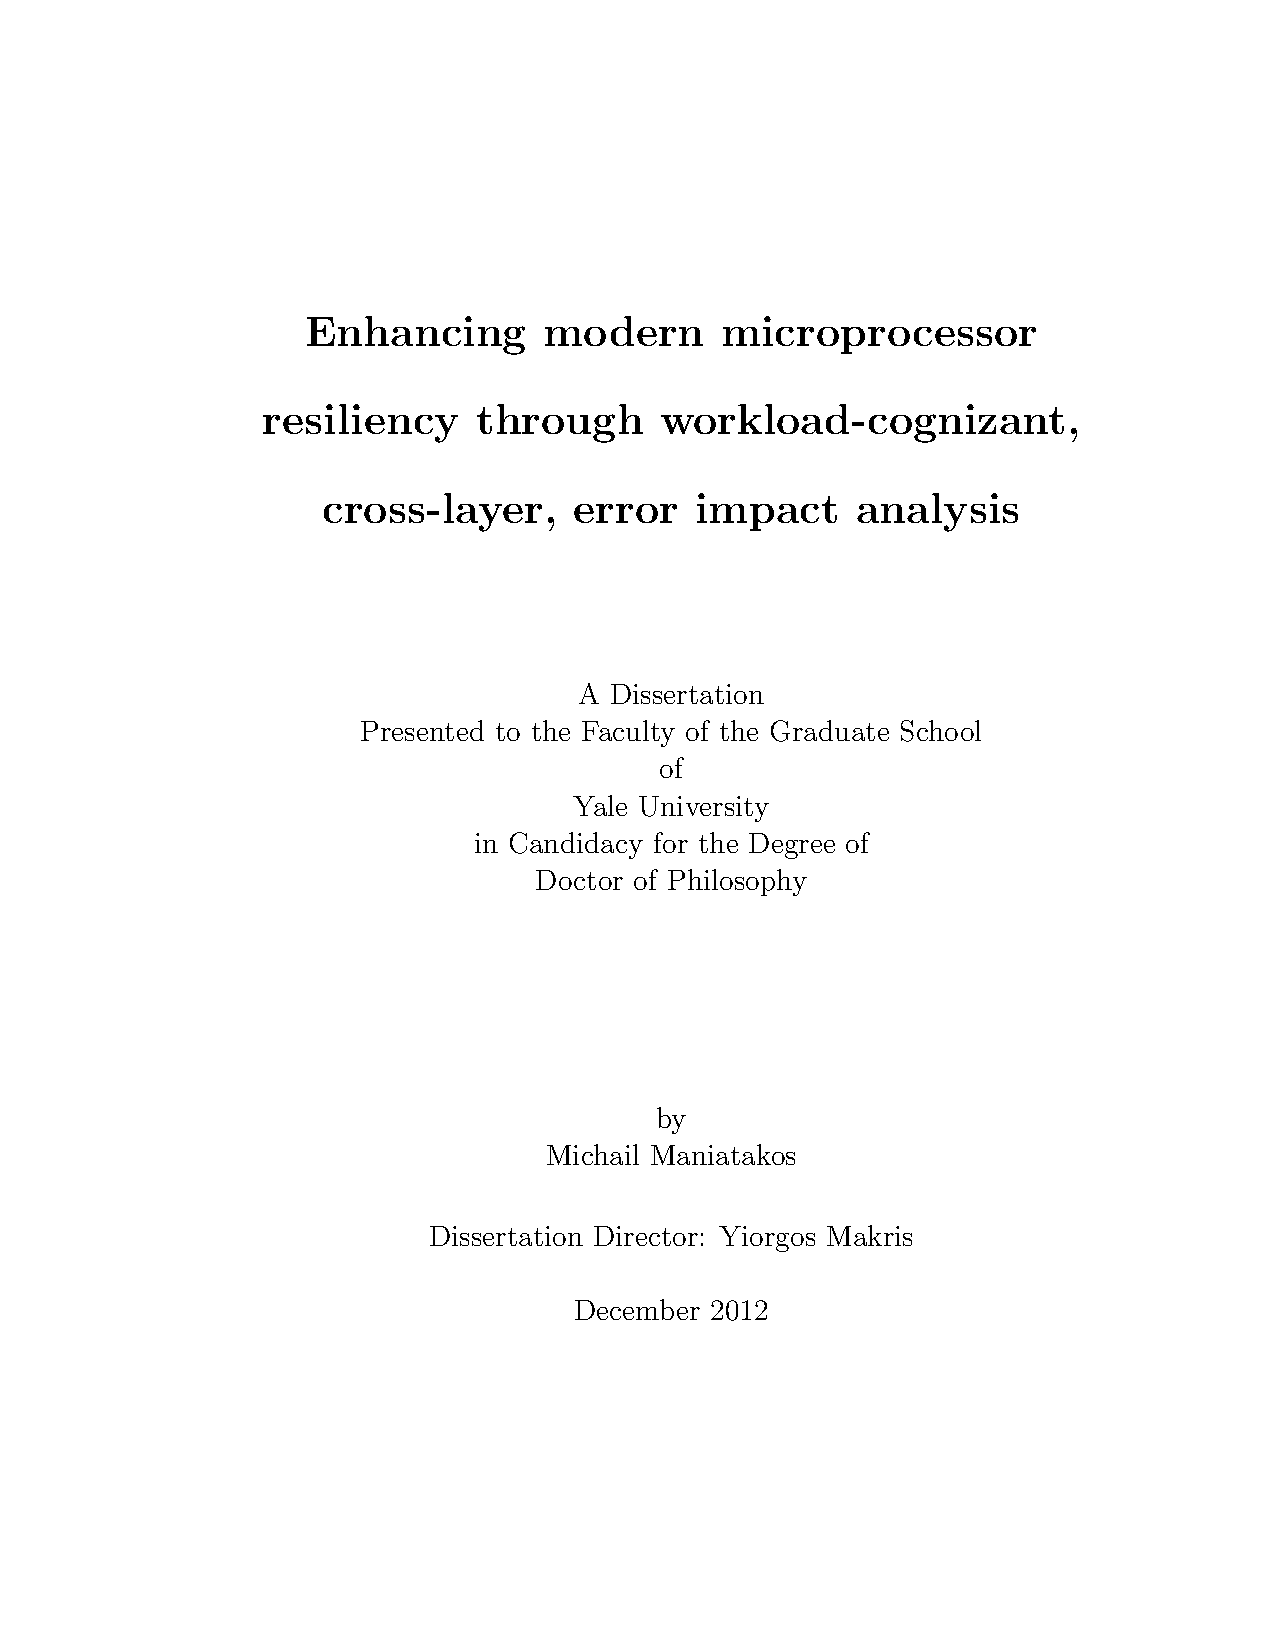
\includegraphics[width=3.5in]{thesis.png}%
\caption{Doctoral thesis outline}%
\label{fOutline}%
\end{figure}

The ability to reason across layers, from transistors to architecture and from events to instructions, serves as the key to developing resiliency enhancing methodologies which extend beyond academic curiosity and become industrially relevant. Consequently, the following main contributions have been successfully demonstrated not only on academic microprocessor models (e.g., IVM) but also on commercial microprocessors (e.g., SUN SPARC, Intel Core). 

\subsection{Cross-layer impact analysis methodology} 
The cornerstone of this doctoral research is a methodology for studying the correlation between low-level faults in a modern microprocessor and their instruction-level impact on the execution of typical workload. Such information is immensely useful in appropriately allocating resources to enhance error/fault resilience through concurrent error detection/correction methods. To this end, an extensive fault simulation infrastructure is developed, which enables injection of stuck-at faults and transient errors of arbitrary starting time and duration, both at the Register Transfer Level and at the Gate Level, as well as cost-effective simulation and classification of their repercussions into various instruction-level error types. As a test vehicle for this study, a superscalar, out-of-order Alpha 21264 microprocessor is employed, with SPEC2000 benchmarks executed as its workload. Extensive fault injection campaigns in key control modules of this microprocessor revealed valuable observations regarding the distribution of low-level faults into the instruction-level error types that they cause. For example, most low-level faults affect the issue or retirement cycle of an instruction, while a very small number of faults affect the retirement order of the instructions. The ability to obtain such information quickly and accurately is crucial towards commensurately allocating resources for ensuring microprocessor robustness in a cost-effective manner.

\subsection{Error detection and correction for microprocessor control logic}
The second chapter of this doctoral thesis focuses on developing concurrent error detection (CED) methods for robustness-sensitive structures of modern microprocessors, such as the control logic. Specifically, a Concurrent Error Detection (CED) scheme for (i) the Scheduler of a modern microprocessor and (ii) the control logic of contemporary floating-point units (FPUs) is developed. The former is based on monitoring a set of invariant properties, violation of which signifies the occurrence of an error. The novelty of the presented solution stems from the workload-cognizant way in which these invariant properties are selected, based on the aforementioned cross-layer impact analysis, so that they leverage the application-level error masking inherent in program execution. At a hardware cost of only 3\% of the Alpha 21264 core, the corresponding CED scheme detects over 85\% of the Scheduler faults that affect the architectural state of the microprocessor. Furthermore, over 99.5\% of these faults are detected before they corrupt the architectural state, implying that the developed technique detects the errors very close to the source. The latter is based on the observation that control logic errors lead to extensive datapath corruption and affect, with high probability the exponent part of the IEEE-754 floating point representation. Indeed, experimental results on the SPARC T1 FPU show that, the developed method incurs an area overhead of only 5.8\%, compared to the 17.9\% of control duplication, yet still achieves detection of over 93\% of transient errors in the FPU control logic. Moreover, the proposed method offers the ancillary benefit of also detecting 98.1\% of the datapath errors that affect the exponent, which cannot be detected via duplication of control logic.

\subsection{Weak-spot assessment and robustness resource allocation prioritization}
A third key contribution of the presented doctoral research is a novel method for assessing the susceptibility of modern microprocessor state elements to failures in the field of operation, which is called Global Signal Vulnerability (GSV) analysis. In order to effectively allocate resources for enhancing robustness, GSV analysis takes into account the high degree of architectural masking exhibited in modern microprocessors and ranks state elements accordingly. The novelty of this method lies in the way this ranking is computed. GSV analysis operates either at the Register Transfer (RT-) or at the Gate-Level, offering increased accuracy in comparison to methods which compute the architectural vulnerability factor (AVF) of registers through high-level simulations on performance models. Moreover, it does not rely on extensive Statistical Fault Injection (SFI) campaigns and lengthy executions of workloads to completion in RT- or Gate-Level designs, which would make such analysis prohibitive. Instead, it monitors the behavior of key global microprocessor signals in response to a progressive stuck-at fault injection method during partial workload execution. Experimentation with the Scheduler and Reorder Buffer modules of both an Alpha 21264 microprocessor and a modern Intel microprocessor (Intel Core) corroborates that GSV analysis generates a near-optimal ranking, yet is several orders of magnitude faster than existing RT- or Gate-Level approaches.

\subsection{Parity selection for in-core memory arrays protection}

This chapter presents an AVF-driven parity selection method for protecting modern microprocessor in-core memory arrays against MBUs. As MBUs constitute more than 50\% of the upsets in latest technologies, error correcting codes or physical interleaving are typically employed to effectively protect out-of-core memory structures, such as caches. However, such methods are not applicable to high-performance in-core arrays, due to computational complexity, high delay and area overhead. To this end, parity is revisited as an effective mechanism to detect errors and pipeline flushing and checkpointing is used for correction. As the optimal parity tree construction for MBU detection is a computationally complex problem, an integer-linear-program (ILP) formulation is used. Experimental results on Alpha 21264 and Intel P6 in-core memory arrays demonstrate that optimal parity tree selection can achieve great vulnerability reduction, even when a small number of bits are added to the parity trees. Furthermore, while the presence of 2 parity trees offers a vulnerability reduction of more than 50\%  over a single parity tree, adding more parity trees does not contribute significantly to the total MBU resiliency enhancement.

Furthermore, after the formulation of the parity selection problem as an ILP, this chapter also presents a cost-effective method for enhancing in-core memory array resiliency, called Vulnerability-based Interleaving (VBI). VBI physically disperses bit-lines based on their vulnerability factor and applies selective parity to these lines. Thereby, VBI aims to ensure that an MBU will affect at most one critical bit-field, so that the selective parity will detect the error and a subsequent pipeline flush will remove its effects. Experimental results employing simulation of realistic MBU fault models on the instruction queue of the Alpha 21264 microprocessor in a 65nm process, demonstrate that a 30\% selective parity protection of VBI-arranged bit-lines reduces vulnerability by 94\%.

\chapter{Impact analysis methodology}\label{sC2}

\section{Introduction}\label{sC2Intro}

While a plethora of microprocessor resiliency enhancement solutions have been developed in the past, blindly applying them across the board is not only prohibitive in terms of cost but also unnecessary in terms of the attained coverage. Indeed, not all faults incur the same level of criticality and not all protection mechanisms contribute equally to the overall robustness of a design. Therefore, methods which analyze the relative importance of potential faults and the relative effectiveness of candidate countermeasures are invaluable for developing cost-effective solutions.

Modern microprocessors, in particular, exhibit an inherent effectiveness in suppressing a significant percentage of faults and preventing them from interfering with correct program execution (i.e. application-level masking). In other words, the probability that a fault will adversely impact the typical workload of a microprocessor varies greatly, depending on the frequency with which the corresponding hardware is used and the complexity of the control conditions necessary to propagate its effect to the architectural state of the microprocessor. Hence, application-level masking presents a great opportunity for developing cost-effective CED methods by identifying and targeting the most critical faults.

To this end, the research described in this chapter seeks to provide the ability to assess the relative importance of low-level faults (i.e. faults in the RT- or Gate-Level description) in the control logic of a modern high-performance microprocessor, as gauged by their impact on the execution of typical programs. Specifically, the contributions of this chapter include:
\begin{itemize}
\item An extensive infrastructure built around a modern microprocessor model, enabling simulation of low-level faults and analysis of their instruction-level impact during execution of typical workload.
\item An instruction-level error model, reflecting the key aspects of instruction execution, to which the impact of low-level faults is mapped.
\item A comprehensive set of fault simulation results demonstrating the correlation between low-level faults in a modern microprocessor controller and the instruction-level errors that they incur.
\end{itemize}

The starting point for developing the aforementioned infrastructure is a public-domain high-performance microprocessor, which is briefly discussed in Section \ref{sC2Existing}. Section \ref{sC2Developed} presents the various components and capabilities of the developed infrastructure, along with its utilization flow for fault injection, simulation and impact analysis. The proposed instruction-level error model, which is used to capture the impact of low-level faults on program execution is introduced in Section \ref{sC2ILEs}. Extensive fault simulation campaigns using the developed infrastructure are presented in Section \ref{sC2Experiments}, along with a detailed analysis of the obtained results and a discussion of their significance in guiding the development of cost-effective CED methods.

\section{Test Vehicle}\label{sC2Existing}

We start by briefly presenting the microprocessor that we will use as the test vehicle in our investigation. We discuss the capabilities of the simulation infrastructure that has been previously developed by other researchers around this microprocessor, we pinpoint its limitations and we identify its components that need to be enhanced in order to support our study.

\subsection{Microprocessor Model and Functional Simulator}
\label{sC2MModel}

Since the focus of this work is the cross-correlation between control logic faults and instruction level errors in modern microprocessors, the underlying test vehicle should incorporate as many of the state-of-the-art architectural features as possible. Among the very limited number of such test-cases available in the public domain, we chose to work with a Verilog implementation of an Alpha-like microprocessor, called IVM (Illinois Verilog Model) \cite{WMP07}. IVM implements a subset of the instruction set of the Alpha 21264 microprocessor, and is rich in architectural features including superscalar, out-of-order execution, dynamically scheduled pipeline, hybrid branch prediction and speculative instruction execution. IVM can have up to 132 instructions in-flight through its 12-stage pipeline, supported by a dynamic scheduler of 32 entries and 6 functional units. The complexity of IVM reflects most of the features of modern, high-performance microprocessors; thus, it enables a realistic investigation of the instruction-level impact of control logic faults in such microprocessors. Besides the Verilog implementation, a functional simulator that can be used in conjunction with the IVM processor model through the Verilog Procedural Interface (VPI) also exists. This functional simulator supports the full set of the Alpha 21264 processor and is part of the SimpleScalar tool suite \cite{BuAu97}.

\subsection{Capabilities and Limitations}

IVM was developed and used to study the impact of single-event transient errors \cite{WMP07,WaPa05,WQRP04}, modeled as single register-level bit-flips. Unfortunately, Gate-Level fault simulation cannot be performed; due to certain coding techniques used at the RT-Level model, IVM is not synthesizable. Instead, an approach of stopping the simulation, altering the state of the microprocessor, and then resuming the simulation was employed in these studies. This fault injection approach is effective when studying the impact of single-cycle transient errors, such as those caused by alpha particle strikes. However, it is extremely inefficient for other fault models, such as stuck-at faults or transient errors of longer duration caused by operational marginalities. Indeed, the process of injecting a fault for a clock cycle involves extensive file-system-based interactions and becomes very time consuming if done for more than a few clock cycles. To alleviate this limitation, we enhanced this infrastructure to support efficient injection and simulation for such longer-lasting faults, as we describe in Section \ref{sC2Developed}.

Another key aspect of the existing infrastructure is that both IVM and the functional simulator can execute software compiled for the Alpha microprocessor. This is important, since it allows us to study the impact of faults while the microprocessor is executing a typical workload, thus making our findings more realistic. However, IVM does not support the full instruction set of Alpha; floating point instructions and various system-calls have not been implemented. Therefore, the functional simulator must be used to surmount this limitation, by invoking it whenever such instructions need to be executed. This interaction is enabled through the ability of the functional simulator to load/store the state of the Verilog model and vice-versa at any given clock cycle.

\section{Enhanced Simulation Infrastructure} \label{sC2Developed}
We now proceed to describe the fault simulation enhancements that we added to the aforementioned infrastructure, as well as the pertinent tool-flow that enables our study. We first outline the main capabilities of the enhanced infrastructure, followed by a detailed description of its basic components and a discussion of its utilization.

\subsection{Capabilities}

We augmented the IVM microprocessor model described in Section \ref{sC2Existing} to provide the following key features:
\begin{itemize}
\item {\bf Workload simulation:} We can simulate software written for the Alpha microprocessor. In our experiments, we use SPEC2000 Integer benchmarks.
\item  {\bf Fault injection \& simulation:} We can perform fault injection into any register or wire entity of the microprocessor by mutating the model accordingly. Fault injection is controlled by a fault controller module inside the microprocessor. The fault simulation infrastructure supports stuck-at faults and transient errors of used-specified start time and duration.
\item {\bf Trace dumping:} The model can produce traces at the periphery of any module of the microprocessor for any user-specified number of clock cycles.
\item {\bf State dumping:} At any given clock cycle, we can save all information concerning the machine state, as well as the architectural state of the processor.
\item {\bf Incorporation of Gate-Level modules:} Synthesizable versions of two modules, namely the Scheduler and the ReOrder Buffer (ROB) have been implemented and can substitute their RT-Level counterparts in the microprocessor model.
\end{itemize}

\subsection{Main Components}

\begin{figure}[!ht]
\centering
\includegraphics[width=2.6in]{parts.png}
\caption{Infrastructure components and interactions}\label{sC2parts}
\end{figure}

The enhanced fault simulation infrastructure consists of three main parts, as shown in Fig. \ref{sC2parts}: i) supporting tools to control fault injection and the I/O of the simulation procedure, ii) a functional simulator of the Alpha microprocessor, and iii) the augmented version of the microprocessor model, where a Fault Controller module has been added to enable Fault Injection.

\subsubsection{Fault Injection Tools}

The main functionality of the fault injection tools is to provide support to the functional simulator by generating the appropriate files and passing parameters for specific operations (e.g. which fault location to inject, the type of injected fault, etc.), as well as accumulating and reporting the simulation results to the user.

Furthermore, the developed tools can be used to save any trace or state files requested and perform comparisons between golden (fault-free) and faulty model executions. The state files contain information regarding the states of all flip-flops and SRAMs in the microprocessor, including the register file and the main memory. The user can choose to extract any subset of the aforementioned storage elements (e.g. only the architectural register file). Besides state files, we can also log the inputs and the outputs of any given module at specified clock cycles, producing a trace file. This file can then be used to study the impact of faults on individual modules. Furthermore, the trace file provides useful statistics about the activation and usage of the I/O of a module, such as identifying the most frequently used wires, their switching frequency etc.

\subsubsection{Functional Simulator}

The presence of a functional simulator in the flow is essential because it enhances the functionality of the microprocessor model. Since the current version of IVM does not implement floating point operations, system calls and miscellaneous other instructions of the Alpha 21264 processor, these instructions can be executed via the functional simulator, which implements the complete instruction set. The simulation can be switched from the functional simulator to the Verilog model and vice-versa at any given time, using VPI calls. In practice, for the SPEC2000 Integer Benchmarks used in this study, the functional simulator is used to skip the initial system calls, after which the execution continues at the RT-level model of the IVM microprocessor.

Furthermore, the functional simulator enhances the I/O functionality of the Verilog model. Thus, it enables reading of values from files and passing parameters to the Verilog model during transition between states. It can also output the state or traces of the microprocessor model to the file system. These features enable fault injection and analysis as well as trace dumping through the developed simulation infrastructure.

\subsubsection{Microprocessor Model}

The microprocessor model used is IVM, which was briefly described in section \ref{sC2MModel}. Since the existing IVM version cannot be synthesized so that gate-level fault injection and simulation can be performed, an alternative way for doing this is required. Even if the complete processor was synthesizable, fault-simulating the entire Gate-Level model would probably be impractical. Hence, we are limited to using RT-Level logic simulation tools, such as Synopsys VCS. This enables simulation of the RT-Level model of the microprocessor while the latter executes actual workload, but it does not offer fault injection capabilities.

To address this limitation, we mutate the IVM model so as to support RT-Level fault injection. Specifically, a Fault Controller module is added to the microprocessor, controlling the fault injection process. When this module is deactivated, the microprocessor operates normally, as a fault-free circuit. When it is activated, however, it provides an extensive range of options for injecting faults. Since the module is already built in the microprocessor model, consecutive simulations injecting different faults can be executed without recompiling the model, something that would make any reasonably-sized fault simulation experiment computationally prohibitive. Besides the insertion of a new module, each existing module of IVM is also mutated to provide support for the functions of the Fault Controller, as explained in detail in Section \ref{sC2Fault_Inj}.

\subsubsection{Fault Controller}\label{sC2Fault-Injection}

\begin{table}[!ht]
\caption{Input/Output interface of fault controller}\label{sC2Fault_Controller}
\begin{center}
\begin{tabular}{||l|l|r||}
\hline
\hline
{\bf Type} & {\bf Name} & {\bf Bits} \\
\hline
Input & fault\_index & 32 \\
\hline
Input & fault\_bit\_index & 8 \\
\hline
Input & fault\_type & 2 \\
\hline
Input & error\_cycle\_start & 32 \\
\hline
Input & error\_cycle\_end & 32 \\
\hline
Output & fault\_register & 42 \\
\hline
Output & fault\_clock & 1 \\
\hline
\hline
\end{tabular}
\end{center}
\end{table}

The main component of fault injection is the embedded Fault Controller module, whose list of inputs and outputs is presented in Table \ref{sC2Fault_Controller} and described below:
\begin{itemize}
\item{\tt fault\_index:} Specifies the unique identification number (UID) of the entity to be fault-injected. Every entity in the microprocessor is assigned a UID. If the UID is invalid, no entity will be fault-injected.
\item{\tt fault\_bit\_index:} Specifies the bit index of the UID to be fault-injected.
\item{\tt fault\_type:} Specifies the type of the injected fault. Our infrastructure supports stuck-at faults and transient errors.
\item{\tt error\_cycle\_start:} Specifies the clock cycle at which the fault injection should commence.
\item{\tt error\_cycle\_end:} Specifies the clock cycle at which the fault injection should terminate.
\item{\tt fault\_register:} Outputs all the information that should be passed to the modules (i.e. {\tt fault\_index, fault\_bit\_index, fault\_type}).
\item{\tt fault\_clock:} The clock that activates fault injection within the modules.
\end{itemize}

By manipulating the data stored in the registers, we can perform single-cycle transient error injection, duration-controlled transient-error injection, or stuck-at fault injection. The registered inputs of the Fault Controller are not connected to and do not interact with the microprocessor model; instead, the functional simulator is responsible for setting these registers to the appropriate values. The output of the Fault Controller propagates to all modules of the microprocessor. In addition, the Fault Controller outputs a clock, which specifies whether a fault should be injected. Specifically, when this clock is 1 each module receives a signal indicating that a fault injection should occur, prompting the module to process the outputs of the Fault Controller.

\subsubsection{Fault Injection}\label{sC2Fault_Inj}

During simulation, the Fault Controller is responsible for fault injection. In each clock cycle, we can access one bit of one entity and set it to a specific value, where the entity can be either a register or a wire. We call this procedure {\em Fault Addressing}. When the Fault Controller activates the fault clock, each module compares the broadcasted UID to the UIDs of its internal entities. If a match is found, the module modifies the corresponding bit, as specified by the outputs of the Fault Controller that are sent to the module. This fault injection technique is similar to the ``parallel saboteurs'' injection technique \cite{JAROK94}. An extensive comparison to existing fault injection approaches can be found in \cite{BGBGG08}.

For a module to be able to respond to Fault Controller functions, it must be mutated accordingly. For this purpose, after assigning a UID to each entity, a piece of code that will enable Fault Addressing within each module must be generated. Moreover, a fault list containing all faults for every bit of each entity must also be generated. Both fault code and fault list generation are performed by internally developed fault injection tools. Depending on whether a module is described as a netlist or as behavioral verilog, the module is mutated differently:

\noindent {\bf RT-Level Fault Injection:} For behavioral Verilog, injection is performed in every entity defined in the Verilog model. Fig. \ref{sC2RT-inject} presents a simplified diagram of the method, which is capable of injecting either stuck-at faults or transient faults, with user-defined starting and stopping times (dotted, lighter colored lines indicate resources added for fault simulation purposes). Since we operate at the RT-Level model, only entities described in the Verilog model are fault-injected. Each entity is driven by a \texttt{MUX}, which is controlled by the Fault Controller. The {\em fault clock} signal alters the value of the target entity during the active fault injection window. Each entity has a unique ID, so that the Fault Controller can pick the one to be injected in each clock cycle.%, while the rest hold their value.

\begin{figure}[!ht]
\centering
\includegraphics[width=3.5in]{RT_inject.png}
\caption{Fault injection in latches of RT-Level model}
\label{sC2RT-inject}
\end{figure}

\noindent {\bf Gate-Level Fault Injection:} Netlist fault injection can also be performed during RT-Level simulation, thereby supporting Gate-Level fault simulation. A simplified version of the method is depicted in Fig. \ref{sC2GT-inject} (dotted, lighter colored lines indicate resources added for fault simulation purposes). In order to avoid cluttering the figure, we only show the resources for 3 out of the 10 fault injection sites; the rest of the sites are injected in the exact same way. In this simulation environment, every wire has an additional driver, which is controlled by the Fault Controller. Cells are treated as black boxes. The Fault Controller drives a high-impedance value \texttt{z} whenever a wire should not be fault-injected, so that the normal value of the wire is propagated. During fault-injection, a \texttt{supply0} or a \texttt{supply1} value is driven on the wire, resembling a stuck-at-0 or a stuck-at-1 fault, respectively. According to Verilog definition, if a wire has multiple drivers the strongest one prevails, with \texttt{z} being a neutral value. \texttt{Supply0} and \texttt{supply1} are the strongest signals, overwriting the regular \texttt{0} or \texttt{1} value of a signal and, thus, injecting a stuck-at fault.

We point out that additional buffers are used in the diagram of Fig. \ref{sC2GT-inject}, in order to enable fault-injection in the various segments of a wire with fanout. These buffers enable individual addressing and, thus, fault-injection on each of the branches of a fanout net. Finally, we also note that in order to successfully simulate a Gate-Level module in an RT-Level environment, the delays of all the standard cells are set to zero, matching the default zero propagation delay of an RT-Level model.

\begin{figure}[!ht]
\centering
\includegraphics[width=3.5in]{GT_inject.png}
\caption{Fault injection in wires of Gate-Level model (resources for 3 out of 10 fault injection sites shown)}
\label{sC2GT-inject}
\end{figure}

\subsection{Simulation Flow}

After presenting each component of the infrastructure, we now describe how these components are combined to provide the aforementioned capabilities. Fig. \ref{sC2flow} presents a flow-chart of the procedure, where each of the three distinct components of Fig. \ref{sC2parts} and their interactions are now depicted in more detail.

\begin{figure}[!ht]
\centering
\includegraphics[width=3.2in]{flow.png}
\caption{Infrastructure utilization flow-chart}
\label{sC2flow}
\end{figure}

Initially, for each entity that will be fault-injected, the corresponding fault code and fault list are added to the IVM model. Fault injection tools initialize the procedure, parse the given fault list and produce the necessary files to guide the functional simulator.

Following the initialization phase, the functional simulator starts execution and parses the fault injection parameters while updating the Fault Controller registers. Once the values are correctly set-up, the functional simulator executes a user-specified number of instructions. Given the fact that IVM lacks system-call support, initial system calls requested by applications must be executed by the functional simulator. When the simulator completes execution, the microprocessor state is transferred to the Verilog model.

The Verilog implementation of the Alpha microprocessor simulates the rest of the program code. After a user-specified number of clock cycles, which is provided through a register in the Fault Controller, the latter activates the fault clock through which it instructs all modules to check whether they should alter any included entity (i.e. perform fault injection during the next clock cycle). At the end of the simulation, the state is saved and transferred back to the functional simulator.

The functional simulator simply outputs the data collected by the Verilog model and stops execution. Subsequently, fault injection tools collect the data and perform the operations requested by the user. We should note that the whole process is very flexible and parameterized; the user can choose functionality (e.g. trace dumping, fault analysis), which faults to inject, when to inject each fault, and how long to inject it for. In this way, various types of studies are facilitated.

\section{Instruction Level Errors} \label{sC2ILEs}

We continue by introducing various types of instruction-level errors (ILEs), organized in several groups. While these ILE types constitute neither a complete nor a mutually exclusively set, they have been carefully selected to reflect incorrect behavior occurring due to faults in the control logic of a modern microprocessor. Thereby, these ILE types enable us to study the correlation between low-level faults in the hardware implementation of control logic and their instruction-level impact.


\subsection{ILE Groups \& Types}\label{sC2ILE_Types}

In this study, we consider thirteen types of ILEs, organized in five distinct groups, as summarized in Table \ref{sC2ILE_Table}. Such grouping reflects the five key aspects of instruction execution in a super-scalar out-of-order microprocessor, namely (i) the operation that is executed, (ii) the operands that are being used, (iii) the functional unit where execution takes place, (iv) the starting and finishing time of execution, and (v) the order of commitment. The various ILE groups and types are discussed in more detail below.


\begin{table}[!ht]
\caption{Instruction-Level Errors (ILEs)}\label{sC2ILE_Table}
\begin{center}
\begin{tabular}{||c|ll||}
\hline
\hline
{\bf Group 1:} & {\bf Type 1:} & Incorrect operation code used\\
\cline{2-3}
Operation Errors & {\bf Type 2:} & Invalid operation code used\\
\hline
\hline
& {\bf Type 3:} & Incorrect register addressed\\
\cline{2-3}
{\bf Group 2:} & {\bf Type 4:} & Invalid register addressed\\
\cline{2-3}
Operand Errors & {\bf Type 5:} & Premature use of register\\
\cline{2-3}
& {\bf Type 6:} & Incorrect immediate operand\\
\hline
\hline
{\bf Group 3:} & {\bf Type 7:} & Incorrect functional unit utilized\\
\cline{2-3}
Execution Errors & {\bf Type 8:} & Multiple functional units utilized\\
\hline
\hline
& {\bf Type 9:} & Early commencement\\
\cline{2-3}
{\bf Group 4:} & {\bf Type 10:} & Late or no commencement\\
\cline{2-3}
Timing Errors& {\bf Type 11:} & Longer duration\\
\cline{2-3}
& {\bf Type 12:} & Shorter duration\\
\hline
\hline
{\bf Group 5:}  & &\\
Order Errors & \raisebox{1.2ex}[0pt]{\bf Type 13:} & \raisebox{1.2ex}[0pt]{Commitment order violation}\\
\hline
\hline
\end{tabular}
\end{center}
\end{table}


\subsubsection{Group 1: Operation Errors}

The first group covers errors in the operation code (op\_code) of the instructions executed by the microprocessor, classified as one of the following ILE types:

\begin{itemize}
\item{\bf{Type 1:}} The op\_code of an instruction is mutated to another op\_code that is valid but incorrect.
\item{\bf{Type 2:}} The op\_code of an instruction is changed to an invalid op\_code.
\end{itemize}

\subsubsection{Group 2: Operand Errors}

The second group covers errors in the operands that are being used by an instruction. In certain instructions, such errors may also affect the instruction execution flow of a program and can, therefore, be considered as control errors. Our error model covers both registers and immediate operands through the following ILE types:

\begin{itemize}
\item{\bf{Type 3:}} A register address used by an instruction points
to a valid but incorrect register file location.
\item{\bf{Type 4:}} A register address used by an instruction
points to an invalid register file location.
\item{\bf{Type 5:}} An instruction uses the contents of a
register prematurely, essentially violating a Read-After-Write (RAW)
constraint.
\item{\bf{Type 6:}} An instruction uses an incorrect immediate value as one of its operands.
\end{itemize}

\subsubsection{Group 3: Execution Errors}
Super-scalar microprocessors employ several functional units of various types (e.g. integer ALUs, floating point ALUs, branch unit, memory operation unit, etc.), in order to execute multiple instructions simultaneously. Accordingly, the third group covers errors in the utilization of these functional units by the executed instruction through the following ILE types:

\begin{itemize}
\item{\bf{Type 7:}} An instruction is assigned to and executed by a functional unit
of incorrect type.
\item{\bf{Type 8:}} An instruction is assigned to more than one
functional unit.
\end{itemize}

\subsubsection{Group 4: Timing Errors}

The fourth group covers discrepancies in the timing of instruction execution. Such discrepancies manifest themselves via incorrect starting and/or finishing instruction execution times and are captured through the following ILE types:

\begin{itemize}
\item{\bf{Type 9:}} An instruction commences execution at an earlier clock-cycle than
it is supposed to.
\item{\bf{Type 10:}} An instruction commences execution at a later
clock-cycle than it is supposed to, or does not commence execution
at all.
\item{\bf{Type 11:}} An instruction completes execution in a longer period of time
than it is supposed to.
\item{\bf{Type 12:}} An instruction completes execution in a shorter
period of time that it is supposed to.
\end{itemize}

\subsubsection{Group 5: Order Errors}

The fifth group covers errors in the order in which instructions are executed and committed. In a processor with out-of-order execution capabilities, the order in which instructions are scheduled and executed does not necessarily follow the program sequence. Therefore, a reorder buffer is typically used to keep track of the instructions that are in flight and ensure that they are committed in order. Errors causing discrepancies in this order are captured by the following ILE type:

\begin{itemize}
\item{\bf{Type 13:}} The correct order of instruction commitment is
violated.
\end{itemize}


\subsection{Classification of Low-Level Faults as ILE Types}

In order to be able to appropriately categorize the impact of a low-level control logic fault into one of the ILE types introduced in the previous section, we use our fault simulation infrastructure to collect the necessary information. More specifically, for each clock cycle, we log various fields related to the execution of instructions in the processor. This is first done once for a golden run, wherein no fault is injected, and subsequently repeated on the fault injected processor for each fault. The two traces of information are compared and, at the first point of failure, the corresponding fields are used to classify the injected fault into an ILE type. The information that is collected from the various modules during each clock cycle is summarized in Table \ref{sC2Classify_Table}. Evidently, the entire microprocessor needs to be simulated in order to accurately assess the impact of a low-level fault on instruction execution. Specifically, the traced information includes:
\begin{enumerate}
\item the op\_code of the instruction being executed; this is simply the type of the instruction. Based on this, ILEs of Types 1-2 can be identified.
\item the physical addresses of the source and destination registers that are used by the instruction; this shows where the operands reside and where the result will be written. Based on this, ILEs of Types 3-4 can be identified.
\item the ready bits of these registers; this indicates whether the source operands are ready to be read. Based on this, ILEs of Type 5 can be identified.
\item the values of any immediate operands that the instruction may be utilizing. Based on this, ILEs of Type 6 can be identified.
\item the identification number of the functional unit where the instruction is executed. Based on this, ILEs of Types 7-8 can be identified.
\item the clock-cycle at which the instruction starts execution. Based on this, ILEs of Types 9-10 can be identified.
\item  the clock cycle at which the instruction is expected to finish execution. Based on this, ILEs of Types 11-12 can be identified.
\item the ROBid of the instruction being executed; this is an identification number assigned by the Reorder Buffer which follows the instruction until it commits and serves as the mechanism for ensuring in-order instruction commitment in the out-of-order execution supported by IVM. Based on this, ILEs of Type 13 can be identified.
\end{enumerate}

\begin{table}[!ht]
\caption{ILE classification information traced from various microprocessor modules}\label{sC2Classify_Table}
\begin{center}
\begin{tabular}{||l|l||}
\hline
\hline
{\bf Module } & {\bf Information} \\
\hline
Decoder & Opcode, Operands, Immediate \\
\hline
Rename & Physical Registers \\
\hline
Execution & Functional Unit Utilization \\
\hline
Scheduler & Issue Time, Replays \\
\hline
Scoreboard & Availability of Operands \\
\hline
Reorder Buffer (ROB) & ROBid, Retirement Cycle/Order \\
\hline
\hline
\end{tabular}
\end{center}
\end{table}

When fault-simulation of a benchmark completes its execution window, automated line-by-line comparison of its trace to the trace of the golden run is performed, as shown in Fig. \ref{sC2ILExample}. In the event of a discrepancy, internally developed tools employ certain checks and algorithms to classify the fault to the appropriate Instruction-Level Error (ILE) type. Even though we compare line-by-line for differences between the golden trace and the faulty trace, when a discrepancy is found, information from multiple cycles is used to correctly classify the error. However, only the first discrepancy is reported and classified as an ILE, because the execution after that point is corrupted and will result in many different ILEs. If more than one ILE are identified in the clock cycle of first ILE appearance, all of them are reported.

\begin{figure}[!ht]
\centering
\includegraphics[width=4in]{ILEclassExample.png}
\caption{Example of classifying a low-level fault as a Type 3 ILE (incorrect register used)}
\label{sC2ILExample}
\end{figure}

\section{Experiments}\label{sC2Experiments}

In this section, we demonstrate the error correlation capabilities and the corresponding insight that can be gained through the developed infrastructure. Specifically, we perform a series of simulations wherein low-level faults (either at the RT- or at the Gate-Level) are injected in the control logic of IVM while the latter executes SPEC2000 benchmarks and we analyze their instruction-level impact. We first discuss the details of the fault simulation setup; then, we present the obtained results and we reflect on the information that they provide and its potential significance in developing cost-effective CED methods.

\subsection{Experimental Setup}
\label{sC2Experimental_Setup}

\noindent {\bf Simulation Workload:} Seven different SPEC2000 benchmarks, namely \texttt{bzip2}, \texttt{mcf}, \texttt{parser},  \texttt{vortex}, \texttt{gzip}, \texttt{gap} and \texttt{cc} are used as the simulation workload. The use of multiple benchmarks ensures variability of the instructions executed through the processor and the control logic that they exercise. Each benchmark is executed by the functional simulator for an initial warm-up period of 50,000 clock cycles, at which point the machine state is transferred to the Verilog model and the execution continues for 2,000 cycles, during which a fault may be injected. On average, 1,297 instructions retire in this window of 2,000 clock cycles.

\noindent {\bf Target Modules:} Since our focus is on microprocessor control logic, we target two key control modules: the Scheduler, which controls the allocation of instructions to execution units, and the ReOrder Buffer (ROB) which controls the order of instruction retirement. Both modules incorporate large buffers to support the number of instructions that can be in-flight, with a combined total of over 40,000 Verilog entities, as shown in Table \ref{sC2RT_level_stats}. The Scheduler is relatively small; it contains 32 slots for instructions waiting to be executed and keeps the information needed to identify and correctly issue an instruction. The ROB is much larger because it contains a 64-slot instruction buffer, as well as complementary information about instruction retirement order.

\begin{table}[!ht]
\caption{Target module details}\label{sC2RT_level_stats}
\begin{center}
\begin{tabular}{||l|r|r|r||}
\hline
\hline
& {\bf \# of} & {\bf \# of} & {\bf \# of} \\
{\bf Module } & {\bf entities} & {\bf stdcells} & {\bf stuck-at faults} \\
\hline
Scheduler & 9,411 & 170,099 & 1,159,012 \\
\hline
ReOrder Buffer (ROB) & 30,735 & 228,881 & 1,714,306 \\
\hline
\hline
\end{tabular}
\end{center}
\end{table}

As shown in Table \ref{sC2RT_level_stats}, the synthesized Scheduler consists of 170,099 standard cells, while the synthesized ROB consists of 228,881 standard cells. Even though the ROB has over 20K (228\%) more storage elements than the Scheduler, it only uses 34\% more standard cells. This is explained since, despite the fact that the ROB uses much larger buffers, the control logic involved is rather small and is only limited to the proper retirement of instructions. On the other hand, the Scheduler performs complicated tasks such as checking whether operands are ready, whether an instruction can be issued avoiding structural hazards etc., which involve much more control logic. The two modules employed in this study are quite diverse, one being a control-logic heavy and the other being buffer-heavy. Hence, we expect the results of our analysis to carry over to other modules that are mainly concerned with instruction execution flow.

\noindent {\bf Injected Faults:} Both stuck-at and transient faults are considered in this study. For the transient fault model, we inject a bit-flip in every simulated clock-cycle, which translates to 2,000 fault simulation runs per fault location.

While simulating the RT-Level versions of the two modules, all entities (presented in Table \ref{sC2RT_level_stats}) are injected. At the gate-level, however, the number of faults is very large, since it includes faults both in the flip-flops and in the combinational logic, so we resort to sampling, with a sample size of $c=30\%$. For the Scheduler, where the total number of faults is $N_{Scheduler}=1,159,012$, this translates to a sample size of $n_{Scheduler}=347,703$ faults, while for the ROB, where  $N_{ROB}=1,714,306$ faults, this translates to a sample size of $n_{ROB}=514,290$ faults. To assess the error incurred due to sampling, we use the following equation, defined in \cite{Ag90}:
\begin{equation}
\label{eq}
C_{0.99} = c \pm \epsilon, \epsilon=\frac{a^2k}{2N_i}\sqrt{1+\frac{4N_ic(1-c)}{a^2k}}
\end{equation}
\noindent where $\epsilon$ is the incurred error, $C_{0.99}$ is the range of fault coverage within which the true coverage lies with a confidence interval of $99\%$, $N_i$ is the total number of faults, $c$ is the fraction of faults to be simulated, $a=2.60$ to achieve a confidence interval of $99\%$, and $k=1$ since the total population is large. Thus, our sample size of $c=30\%$ yields an error of $\epsilon=0.01\%$, which is more than adequate for the purpose of our analysis.

\noindent {\bf Computational Power:} The experiments are performed on a Quad-core Xeon 3.33GHz with 16GB of memory.


\subsection{Results and Analysis}\label{sC2Results}

In this section we present the results of evaluating the impact of low-level faults on the instruction-level. The results are divided in three subsections:

\begin{enumerate}[i)]

\item First, we present results which reveal the correlation between RT-Level faults and the instruction-level errors that they cause.

\item Second, we present a comparative analysis of the impact of RT- vis-a-vis Gate-Level faults on instruction-level execution. These results corroborate that the above correlation remains valid independent of the level at which fault injection is performed.

\item Third, we present a comparative analysis of the impact of stuck-at faults vis-a-vis transient errors. Once again, the results corroborate that the correlation between low-level faults and instruction-level errors holds true, independent of the injected fault type.

\end{enumerate}

\subsubsection{Instruction-Level impact of RT-Level stuck-at faults}\label{sC2InstImpact}
\snp{Fault Simulation Statistics:} As a first set of results, we present cumulative data regarding the fault simulations performed. Specifically, Table \ref{sC2SPEC_stats} reports the percentage of the 80,804 injected faults (for both the Scheduler and the ROB) that resulted in an ILE, as well as the average number of ILE types that are simultaneously activated for each of the seven SPEC2000 benchmark programs that were executed. 

\begin{table}[!ht]
\caption{Results on SPEC2000 Integer Benchmarks}\label{sC2SPEC_stats}
\begin{center}
\begin{threeparttable}[b]
\begin{tabular}{||c|c|c||}
\hline
\hline
{\bf } & {\bf }  &\bf{Average \# of} \\
{\bf } & {\bf Faults Resulting}  &\bf{ILEs Activated} \\
{\bf SPEC Benchmark} & {\bf in ILEs\tnote{1}}  & \bf{Simultaneously} \\
\hline
bzip2 & 39.3\% (98.6\%) &  1.32 \\
\hline
mcf & 16.6\% (98.2\%) &  1.19 \\
\hline
parser & 42.0\% (99.9\%) &  1.39 \\
\hline
vortex & 39.2\% (99.8\%) &  1.10 \\
\hline
gzip & 17.4\% (99.4\%) &  1.26 \\
\hline
gap & 17.0\% (99.9\%) &  1.14 \\
\hline
cc & 38.2\% (99.5\%) &  1.31 \\
\hline
\hline
{\bf Average} & {\bf 29.9\% (99.3\%)} &  {\bf 1.24}  \\
\hline
\hline
\end{tabular}
  \begin{tablenotes}
    \item[1] The percentage shown in the parenthesis is the percentage of faults resulting in an ILE that also corrupt the architectural state of the microprocessor in the injection period.
  \end{tablenotes}
\end{threeparttable}
\end{center}
\end{table}

Based on this table, the following observations can be made:

\begin{itemize}
\item The number of faults resulting in an ILE ranges between 16\%-42\%. Intuitively, faults injected during the execution of benchmark programs using a limited variety and algorithmic combination of instructions will excite fewer ILEs due to a larger portion of unused processor functionality. Certain register bits are rarely used in a typical execution flow (e.g. the most significant bits of address registers, or scheduler slots that are used only when a fairly large number of instructions are in flight). This high percentage of application-level masking highlights the advantage of using workload information to develop efficient CED techniques.

\item Among the faults resulting in an ILE, an average of 99.3\% also cause an architectural error. This high percentage elucidates the fact that the proposed ILE types constitute an effective way of capturing incorrect workload execution. The few faults that cause an ILE but do not affect the architectural state area attributed to either architectural masking (e.g. a fault that corrupts an instruction which never commits due to speculative execution) or performance faults (e.g. a fault that delays the availability of a functional unit and causes the workload to take longer to execute). We also note that, in our experiments, none of the faults may result in an incorrect architectural state but not cause an ILE.

\item Since the ILE types are not mutually exclusive, more than one ILE types may be activated simultaneously, even when checking in a cycle-by-cycle fashion. However, as can be observed in the last column of Table \ref{sC2SPEC_stats}, the average number of simultaneously activated ILE types is only 1.24; this implies that, most of the time, only one of the 13 ILE types is activated at the first point of failure. The implication of this information is that corruption will typically occur only at one aspect of instruction execution, with the rest remaining unaffected. Thus, early detection of such ILEs can guide simple local operations towards restoring the correct state of the microprocessor.
\end{itemize}

\snp{Benchmark Consistency:} Our second set of results examines the consistency of the information provided through our experiments. Specifically, since each benchmark utilizes different functional capabilities of the processor, the ILE type resulting from a stuck-at fault may vary, depending on the actual instructions being executed. In this sense, the robustness of the error correlation information may be questioned. Therefore, in Fig. \ref{sC2robustness}, we present the percentage of stuck-at faults that results in ILEs of each of the five groups described in Section \ref{sC2ILE_Types}, for each of the seven benchmark programs. 

\begin{figure}[!ht]
\centering
\includegraphics[width=3.5in]{Fig9-1-2.png}
\caption{Percentage of stuck-at faults causing each ILE group for each of the seven benchmarks}
\label{sC2robustness}
\end{figure}

Based on this bar-chart, the following observations can be made:
\begin{itemize}
\item The distribution of stuck-at faults to the five groups of ILEs is consistent across the seven benchmarks. Furthermore, the variance of stuck-at faults within each group across the seven benchmarks is small. These observations corroborate that the obtained error correlation information is not biased by the actual instructions executed by each benchmark program and is, therefore, robust.
\item A large percentage of stuck-at faults (60\%-75\%) result in timing errors in all benchmarks, implying that, independent of the workload utilized, most stuck-at faults in the control logic may not affect the instruction itself but, rather, when this instruction is executed. This is expected since faults injected in the Scheduler and the ROB modules directly impact instruction issuing and commitment. Such information is very useful in guiding allocation of error detection and recovery resources. In this case, for example, one would focus on methods that predict and monitor the correctness of instruction starting and stopping times, since, thereby, the majority of the faults would be detected.
\end{itemize}

\snp{ILE Distribution:} The third set of presented results relates to the occurrence frequency of each of the 13 ILE types described in Section \ref{sC2ILE_Types}. The average number of stuck-at faults resulting in each ILE type over the seven benchmarks is presented in Fig. \ref{sC2results_types}. The subset of these faults that eventually result in stalling of the pipeline is also provided. The following observations can be made based on the results:

\begin{itemize}
\item The most frequently occurring ILEs concern instruction execution timing. Specifically, late instruction commencement (Type 10) and longer instruction duration (Type 11) are the dominant types. In other words, faults injected in the Scheduler and the ROB module will often result in failure to issue an instruction or failure to commit an instruction at the appropriate clock-cycle. Another interesting observation is the frequent appearance of operand mutations (Type 3). Indeed, the complex structures employed by the scheduler to keep track of the 1 to 3 registers used by each instruction, appear to be vulnerable to various stuck-at faults in the control logic.
\item On the other hand, stuck-at faults in the Scheduler and the ROB seem to rarely cause mutation of operation codes (Type 2) or invalid operand address (Type 4), since the logic involved is relatively limited. Similarly, very few faults cause premature use of operands (Type 5), incorrect functional unit assignment (Types 7-8), or out-of-order instruction commitment (Type 13). In these cases, the involved logic can be large, but its complexity is such that it prevents single stuck-at faults in a register from activating these ILE types, hence their low occurrence probability.
\item Among the faults resulting in an ILE most (up to 80\%) lead to a pipeline stall. In other words, while the initial error may only manifest in one aspect of instruction execution, if the error is not corrected promptly it will most likely have an avalanche effect that will eventually stall the processor. Moreover, our intuition is that the reported percentage is an under-estimate due to the limited fault simulation window of 2,000 cycles.
\end{itemize}

The insight provided by the aforementioned observations regarding the most frequently occurring and, thus, the most critical ILE types can be leveraged to facilitate cost-effective use of error detection and correction resources. by implementing small, efficient CED techniques targeting specific ILE types.

\snp{ILE Appearance Time:} Another very interesting set of results pertains to the time that elapses between injection of a fault and its appearance as one of the defined ILE types, as well as the latency between appearance of an ILE and a potential subsequent stalling of the microprocessor. This information is provided in Fig. \ref{sC2results_times}. While the activation time of an ILE may depend on the actual sequence of executed instructions, averaging the results over the seven SPEC2000 benchmarks provides an unbiased estimate. The obtained results motivate the following observations:

\begin{figure}[!ht]
\centering
\includegraphics[width=3.5in]{Fig9-1-3.png}
\caption{Average number of stuck-at faults causing each ILE Type and subsets causing stalled execution}
\label{sC2results_types}
\end{figure}

\begin{itemize}
\item The average time until an injected fault results in an ILE is 406 clock cycles. However, the standard deviation across the 13 ILE types is rather high (198 clock cycles), with some ILE types occurring very quickly and others much later. For example, invalid operation code (Type 2), utilization of multiple functional units (Type 8) and incorrect commitment order (Type 13) are types of ILEs appearing very quickly after fault injection. Indeed, despite the fact that the set of faults causing these ILEs is relatively small (as presented in Fig. \ref{sC2results_types}), such faults are directly associated with these specific types of ILEs. Thus, upon the appearance of such a fault, the corresponding ILE is immediately activated. On the other hand, ILEs related to timing issues (e.g. Types 9-11) appear much later. Such ILEs seem to be often the result of faults propagating to parts of the microprocessor that do not interfere directly with the main pipeline flow, yet eventually work their way into it and, hence, the longer latency.
\item On average, a microprocessor stall occurs 280 clock cycles after occurrence of an ILE. However, one may observe that some ILEs concerning timing issues (i.e. Types 9-11) result in microprocessor stalling much faster than the rest of the ILEs; given the fact that these ILEs are caused when the Scheduler or the ROB fail to timely issue or commit an instruction, subsequent instructions fail to issue or commit successfully, inevitably causing the pipeline to stall very quickly. On the other hand, for ILEs such as Type 7, stalling appears much later, after the Scheduler and/or the ROB fill up with instructions waiting for the incorrectly executed instruction to retire. \end{itemize}

The insight provided by the aforementioned observations is two-fold. First, they reveal the relative temporal criticality of each ILE type. Thus, they can be used to fine-tune error tolerance methods that employ checkpoints to examine and restore the microprocessor state \cite{WaPa05}. Second, they indicate the window of opportunity for correcting an error before it drastically corrupts the processor state and results in a stall. Thus, they can be leveraged to prioritize the allocation of error detection and correction resources.

Finally, Fig. \ref{sC2results_times} shows that the activated ILEs appear no later than 1,200 cycles after fault injection; this ensures that the window of 2,000 clock cycles that we observe is sufficiently long for the performed analysis. While ILEs that would require a much larger simulation window to appear may exist, their number is relatively small and would not alter the profile of the results.


\begin{figure}[!ht]
\centering
\includegraphics[width=3.5in]{Fig9-1-4.png}
\caption{Average time-stamp of ILE identification and subsequent pipeline stalling (in clock cycles)}
\label{sC2results_times}
\end{figure}

\subsubsection{Impact comparison of RT- vs. Gate-Level faults}

\snp{Impact consistency:} The first set of results compares the accuracy of assessing the impact of low-level faults on instruction execution at the RT- vs. the Gate-Level. Specifically, Fig. \ref{sC2Sch_ILEs} and \ref{sC2ROB_ILEs} present the classification of RT- and Gate-Level faults into the ILE types that they cause, for each of the seven benchmarks. The results are presented separately for the Scheduler and the ROB since the Scheduler is a control logic-heavy module whereas the ROB is a buffer-heavy module. 

\begin{figure}[!ht]
\centering
\subfloat[Scheduler]{\includegraphics[width=2.9in]{Fig9-2-1.png}\label{sC2Sch_ILEs}}
\subfloat[ROB]{\includegraphics[width=2.9in]{Fig9-2-2.png}\label{sC2ROB_ILEs}}
\caption{Comparison between ILE Types caused by RT- vs. Gate-Level faults}
\end{figure}

Based on the results, we can make the following observations:

\begin{itemize}
\item The most important observation is a pronounced consistency in the types and frequency of ILEs caused by RT- vs. Gate-Level faults. Indeed, for each benchmark, the distribution of RT-Level faults to the 13 ILE types is strongly correlated with the distribution of Gate-Level faults to the same, as presented in Table \ref{sC2SPEC_stats_VTS}. On average, the correlation coefficient\footnote{If $R$ is the vector containing the 13 values representing the percentage of the faults that result in each ILE Type for the RT-Level, and $G$ is the same vector for the Gate-Level ($\bar{R}$ and $\bar{G}$ being the respective average values) then the correlation coefficient $c$ is calculated as:

    \begin{center}
    $c = \displaystyle\frac{\sum_{n=1}^{13}{(R_n-\bar{R})(G_n-\bar{G})}}
    {\sqrt{(\sum_{n=1}^{13}{(R_n-\bar{R})^2})(\sum_{n=1}^{13}{(G_n-\bar{G})^2})}}$
    \end{center}} is 93\% for both the Scheduler and the ROB. This critical observation corroborates that RT-Level fault analysis provides sufficiently accurate results with respect to its Gate-Level counterpart.

\begin{table}[!ht]
\begin{center}
\begin{threeparttable}[b]
\caption{Results on SPEC2000 Integer benchmarks}\label{sC2SPEC_stats_VTS}
\begin{tabular}{||c|c|c||}
\hline
\hline
{\bf SPEC}      & {\bf Correlation}   & {\bf Correlation} \\
{\bf Benchmark} & {\bf Coefficient}   & {\bf Coefficient} \\
{\bf Name}      & {\bf for Scheduler\tnote{1}} & {\bf for ROB\tnote{1}}     \\
\hline
bzip2  & 91.66\% & 94.07\% \\
\hline
mcf    & 96.29\% & 93.32\% \\
\hline
parser & 92.47\% & 91.63\% \\
\hline
vortex & 93.96\% & 93.84\% \\
\hline
gzip   & 93.02\% & 90.96\% \\
\hline
gap    & 94.65\% & 95.74\% \\
\hline
cc     & 95.60\% & 93.46\% \\
\hline
\hline
{\bf Average} & {\bf 93.95\%} & {\bf 93.29\%} \\
\hline
\hline
\end{tabular}
\end{threeparttable}
\end{center}
\end{table}

\item The next observation is that the distributions are consistent across the various benchmarks, confirming the results presented in the previous section. Hence, it is evident that the type of ILE caused by a low-level fault is, typically, independent of the instruction subset that is utilized.

\item A final observation is that some ILE types appear never to be caused by Gate-Level faults. These ILE types have already a very small frequency of occurrence due to RT-Level faults, which is further diminished during Gate-Level fault simulation because of sampling.
\end{itemize}


\snp{Fault simulation speed:} The next set of results investigates how the simulation speed is affected by the use of Gate-Level modules. Table \ref{sC2Simulation speed} compares the average simulation time per fault for the various configurations. The first row provides the baseline, where all modules are simulated at the RT-Level, while the following rows indicate the overhead when one or both of the target modules are simulated at the Gate-Level. As may be observed, this makes the simulation over an order of magnitude slower. Taking into account that, even with 30\% fault sampling, using the Gate-Level Scheduler and ROB requires, on average, 5.8x (5.0x for Scheduler, 6.6x for ROB) more fault simulations than their RT-Level counterparts, a similar fault analysis at the Gate-Level is 260x more expensive, rendering it almost infeasible for extensive studies. Therefore, performing the simulations at the RT-Level is strongly desired, especially since the accuracy of the obtained results is up to par, as confirmed by the above results.

\begin{table}[!ht]
\centering
\begin{threeparttable}[b]
\caption{Fault simulation speed comparison}\label{sC2Simulation speed}
\begin{tabular}{||l|c|c|c|c||}
\hline
\hline
                &                  & {\bf Time}     & {\bf }          & {\bf Overall} \\
{\bf Fault}     & {\bf Seconds }   & {\bf Overhead} & {\bf Number of} & {\bf Overhead} \\
{\bf Simulated} & {\bf per Fault}  & {(Comp.}       & {\bf Simulated} & {(Comp.}  \\
{\bf Modules}   & {\bf Simulation} & { to RTL)}     & {\bf Faults\tnote{1} }   & { to RTL)}  \\

\hline
All RTL    &       &       &         &        \\
modules    & 3.26  & -     & 80,292  & -      \\
\hline
Gate-level &       &       &         &        \\
Scheduler  & 35.04 & 10.7x & 407,173 & 54.5x  \\
\hline
Gate-level &       &       &         &        \\
ROB        & 42.20 & 12.9x & 533,112 & 85.9x  \\
\hline
Gate-level &       &       &         &        \\
Sch., ROB  & 79.02 & 24.2x & 861,993 & 260.2x \\

\hline
\hline
\end{tabular}
  \begin{tablenotes}
    \item[1] The Gate-Level fault list is a 30\% uniform sample
  \end{tablenotes}
\end{threeparttable}
\end{table}

\subsubsection{Impact comparison of stuck-at vs. transient faults}

\snp{Transient fault classification:} We now compare the impact of two different fault models, namely stuck-at faults and bit-flip transients, on instruction execution. We note that, while classifying the impact of a stuck-at fault to an ILE is rather straightforward, doing so for a transient fault is more complicated. Indeed, transients in the same location may result in a different ILE type depending on the time of fault injection during the simulation. Therefore, for each fault we perform 2,000 simulations, each time injecting it at a different clock cycle and we collect the probability with which this fault will lead to an ILE of each type. For example, assume that a stuck-at fault in a register causes an ILE of Type 3, while a bit-flip in the same register results in an ILE of Type 3 if injected in clock cycles 10, 500 or 1200 and as ILE of Type 11 if injected in clock cycles 250 or 1500. Then, this transient fault contributes 0.6 to the number of transient faults that result in an ILE of Type 3 and 0.4 to the number of transient faults that result in an ILE of Type 11. In contrast, the corresponding stuck-at fault contributes 1 to the number of faults resulting in an ILE of Type 3.

\snp{Impact consistency:} Fig. \ref{sC2Stuck-Trans} shows the combined results for the Scheduler and the ROB for the 7 different benchmarks. The results reveal a very high consistency between the distribution of stuck-at and transient faults to the corresponding ILEs (i.e. an average correlation coefficient of 98\%). This consistency can be further explained by examining the impact of individual transient faults. While a transient may result in various ILE types depending on its time of injection, it turns out that, most of the time (over 80\% on average), it causes the same ILE. Hence, even if one is interested in developing CED methods for transient bit-flips, assessing their instruction-level impact through stuck-at fault simulations would provide sufficiently accurate results. Moreover, as explained in the previous paragraph, assessing instruction-level impact through simulation of stuck-at faults is far less time-consuming than through transient faults, since only one simulation is necessary per fault location.

\begin{figure}[!ht]
\centering
\includegraphics[width=2.9in]{Fig9-3-1.png}
\caption{Comparison between ILE Types caused by stuck-at vs. transient faults in the Scheduler and the ROB}
\label{sC2Stuck-Trans}
\end{figure}

\section{Conclusions}
In order to develop cost-effective CED methods which leverage the ability of modern microprocessors to suppress a high percentage of errors at the application level, a thorough understanding of the impact of low-level faults on program execution is necessary. To this end, the infrastructure reported herein, which we developed around an Alpha-like high-performance microprocessor, enables injection, simulation and classification of low-level faults into instruction-level error types. Extensive experimentation with this infrastructure provided great insight regarding the relative importance of low-level faults, as gauged by the activation frequency and latency of the instruction-level error types that they cause. Furthermore, it revealed a profound instruction-level impact consistency between RT- and Gate-Level faults, as well as between stuck-at and transient faults. Besides CED, the capabilities of the developed infrastructure may be utilized to provide similar insight and guidance for various other design robustness endeavors.

\chapter{Error detection and correction for microprocessor control logic}\label{sC3}

\section{Introduction}

The pluralism of Concurrent Error Detection (CED) methods that have been proposed in the past implies that no one solution fits the needs of every circuit. Furthermore, it stresses the fact that applying generic solutions across the board for an entire design typically incurs prohibitive cost, often times unnecessarily and without providing commensurate coverage. Indeed, in order to maintain cost-effectiveness, it is important to understand the specific vulnerabilities and requirements of a circuit and accordingly tailor the CED solution.

Modern microprocessors, as discussed in Section \ref{sC2Intro}, exhibit a high degree of application-level error masking. Indeed, the multitude of functional units and stages in deeply-pipelined superscalar microprocessors, along with advanced architectural features such as dynamic scheduling and speculative execution, imply that rather complex conditions need to be satisfied for an error to affect the architectural state of the microprocessor. Furthermore, it is well-known that the probability with which faults are suppressed is asymmetric \cite{Mo03b}, implying that not all faults are equally critical. Hence, high-level methods that aim to globally monitor the most susceptible aspects of instruction execution, rather than to locally check the result of every fine-grain hardware entity, appear to be the most promising direction towards developing cost-effective CED solutions.

To this end, we leverage the information provided by the workload-cognizant, cross-layer impact analysis methodology presented in Chapter \ref{sC2} to develop cost effective CED solutions for the control logic of the main processing units of a modern chip: The Central Processing Unit (CPU), presented in Section \ref{sC2CEDCPU}, and the Floating-Point Unit (FPU), presented in Section \ref{sC2CEDFPU}.

\section{CED for CPU controllers}\label{sC2CEDCPU}

\subsection{Introduction}

In this section, we develop a workload-cognizant CED scheme for the Scheduler of a modern microprocessor, based on detailed information regarding the impact of faults on the instruction execution of typical programs. Specifically, we use the infrastructure and the results presented in Chapter \ref{sC2} in order to understand the relative importance of the various ILEs that are caused by faults in the Scheduler of the microprocessor. Guided by the results of this analysis, we incorporate additional hardware that monitors the most vulnerable aspects of instruction execution. Specifically, we predict and validate the time and the functional unit where an instruction is executed, along with four hardware-imposed {\em invariances} (i.e. properties which hold true during error-free operation but which are violated in the presence of errors), which validate the operation code and the operands of an instruction, as well as the sequence in which instructions are executed and retired. Extensive fault simulation-based evaluation validates that workload information can, indeed, drive the development of cost-effective CED methods.

The remainder of this section is organized as follows. In section \ref{sC3sPrevious} we discuss related work in CED. Then, in section \ref{sC3sScheduler}, we provide more details about the Scheduler of this microprocessor, which is the target of our CED scheme. The details of the developed CED scheme are given in section \ref{sC3sCED}. Finally, extensive fault simulation results demonstrating the effectiveness of the proposed CED scheme are presented and discussed in section \ref{sC3sResults} and conclusions are drawn in section \ref{sC3sConclusion}.

\subsection{Related Work}\label{sC3sPrevious}

Various CED solutions \cite{GoGr93,MiMc00} have been proposed in the past to detect faults or errors occurring during normal operation of a circuit after it is deployed in the field. Among those, the simplest approach is duplication, wherein a replica of the circuit is added to the design, possibly diversely implemented (e.g. through the use of dual-rail logic \cite{923436}) to avoid common mode failures \cite{AvKe84}. The original and the replica serve as predictors of the functionality of each other and a simple comparator indicates any discrepancy in their outputs, thus detecting potential malfunctions. While simple, this technique is prohibitively expensive. To reduce the overhead imposed by duplication-based techniques, partial duplication has been suggested to detect the faults in the most critical parts of the design \cite{Mo03b}.

Another very popular CED approach has been the use of various codes, especially within the context of finite state machine (FSM) controllers. Several redesign and resynthesis methods are described in \cite{AkSo75, DhVr88}, wherein parity or various unordered codes are employed to encode the states of the circuit. Utilization of multiple parity bits is also examined in \cite{ZSM98} within the context of FSMs. These methods guarantee latency-free error detection; on the down side, they are intrusive and expensive. Non-intrusive CED methods have also been proposed. Implementations based on Hamming, Bose-Lin and Berger codes are presented in \cite{1030186}, \cite{670885} and \cite{229762}, respectively, while parity-based CED methods are described in \cite{GoGr93,ADM06,1676055}. While the aforementioned methods guarantee latency-free detection of all errors, their cost is often prohibitive. Trading-off the incurred cost by allowing a non-zero, yet bounded error detection latency has also been investigated \cite{AMD04}.

At a coarser level, an attempt to identify inherent invariance either at the gate-level \cite{VJAPG08} or at the RTL \cite{1308673} of a design has been made. Such invariance can be monitored during the normal operation of a circuit to identify errors that cause it to be violated. In \cite{VJAPG08} such invariance is mined from the gate-level of a controller implementation in the form of assertions, which are evaluated through simulation in order to select a cost-effective appropriate subset. The same principle governs the approach in \cite{1308673}; therein, however, invariance is identified through a path-construction algorithm, which exploits inherent transparency channels that exist in the RTL description of a modular design. More recently, the method proposed in \cite{MROJG08} also leverages inherent invariant codes to perform CED in the decoder of the same microprocessor that we employ in this study.

At an even higher architectural level, several concurrent error detection and/or correction methods have been proposed. The concept of watchdog processors, which compute control-flow signatures and compare them to expected correct values, known at compilation time, is proposed in \cite{2145,JN08}. Concepts akin to instruction-level duplication and comparison to identify erroneous results are examined in \cite{MeSu00,941424}. In \cite{WQRP04}, the authors examine the vulnerability of different parts of a microprocessor to soft errors and recommend various strategies (including register file protection with codes, parity coding to protect instruction words, and a timeout counter to flush the pipeline when no activity occurs for prolonged periods) to detect/correct such errors. Similar analysis is performed in \cite{MWERA03}, based on the concept of Architectural Vulnerability Factor (AVF), which prioritizes microprocessor modules based on their susceptibility. Such metrics can prove very useful in guiding allocation of CED resources.

\subsection{Scheduler Module}\label{sC3sScheduler}

The Scheduler is one of the key control modules in any modern microprocessor with advanced architectural features. In IVM, the Scheduler is a dynamic module containing an array of up to 32 instructions waiting to be issued, from which up to 6 instructions are issued in each clock cycle. Each instruction coming to the Scheduler resides in this buffer until an acknowledgment is received from the execution unit that it can start execution. At this time, the corresponding location in the Scheduler waiting-list is cleared for use by another newly arriving instruction. The Scheduler issues instructions out-of-order after considering the availability of instructions of various types in the buffer, as well as the existence of structural or data hazards.

During instruction execution, avoidance of structural and data hazards is ensured by the Scheduler, while avoidance of control hazards is ensured by the Reorder Buffer (ROB). Indeed, the Scheduler considers structural hazards before issuing an instruction. The IVM microprocessor has 6 functional units: 2 simple, 1 complex, 1 branch and 2 memory units. Thus, up to 6 instructions with the above limitations on the type and distribution of instructions can be issued in each clock cycle. Write-After-Read (WAR) and Write-After-Write (WAW) data hazards are taken care of by the Rename module of IVM before the instruction comes to the Scheduler. Read-After-Write (RAW) data hazards, however, may still exist due to dependencies between instruction operands. To deal with such RAW hazards, the Scheduler uses the Scoreboard method \cite{hennessy2011computer}. Based on the type of functional unit that will be executing an instruction, the Scoreboard determines the clock cycle in which the destination register for this instruction will be written and available for other instructions to read. Consequently, the Scheduler prevents issuing of instructions that need to use this register prior to the time that it becomes available. Along with each instruction coming to the Scheduler from the Rename module, a unique identification number called ROBid is also provided by the ROB module. This ROBid follows the instruction until it commits and serves as a mechanism for ensuring in-order instruction commitment in the out-of-order execution of the microprocessor and avoiding control hazards.

Figure \ref{sC3Scheduler} shows the high level diagram of the IVM Scheduler module. As shown in this figure, instructions arriving to the Scheduler continue to reside in the buffer even if they have been issued to the Execution unit, until the execution unit confirms that they can start execution. At this time the ``valid" and ``issued" signals of the related instruction in the Scheduler are disabled and the corresponding buffer locations are considered available for use by subsequent instructions.

\begin{figure}[!ht]
\centering
\includegraphics[width=5.95in]{Fig-3.png}
\caption{Block diagram of IVM Scheduler}\label{sC3Scheduler}
\end{figure}

\subsection{Scheduler CED Scheme}\label{sC3sCED}

Based on the observations presented in Section \ref{sC2InstImpact}, where timing errors where identified as dominant, the timestamp-based CED scheme proposed in this section seeks to verify the following aspects of instruction execution, which are listed in decreasing order of significance:

\begin{itemize}
\item Correctness of the time at which an instruction starts executing.
\item Correctness of the operands used by the instruction.
\item Correctness of the operation code executed by the instruction.
\item Correctness of the sequence in which instructions are actually executed, taking into account branches.
\item Correctness of the sequence in which instructions arrive to the scheduler.
\item Correctness of the functional unit to which an instruction is assigned for execution.
\end{itemize}

To achieve the above objectives, the proposed CED scheme involves two components. The first component employs additional hardware which predetermines the time at which an instruction should start execution and the functional unit where it should be executed, as explained in Section \ref{sC3sTimePlace}. Using this information, the second component employs additional hardware to impose and monitor four invariances that should hold true in each clock cycle $i$ and for each functional unit $j$:

\begin{itemize}
\item {\bf Invariance \#1:} Equality between the ROBid of the instruction that is predicted to be executed at time $i$ by functional unit $j$ and the ROBid of the instruction that is actually executed. Monitoring this invariance ensures correct order in the commitment of instructions. Thereby, this invariance aims mainly at detecting ILEs of Group 5 (Order Errors).

\item {\bf Invariance \#2:} Parity consistency between the operation code of the instruction that is predicted to be executed at time $i$ by functional unit $j$ and the operation code of the instruction that is actually executed. This invariance aims mainly at detecting ILEs of Group 1 (Operation Errors).

\item {\bf Invariance \#3:} Parity consistency between the operands (up to three) of the instruction that is predicted to be executed at time $i$ by functional unit $j$ and the operands used by the instruction that is actually executed. This invariance aims mainly at detecting ILEs of Group 2 (Operand Errors).

\item {\bf Invariance \#4:} Parity consistency between the target address of the instruction that is predicted to be executed at time $i$ by functional unit $j$ and the target address of the instruction that is actually executed. Checking this invariance ensures the correctness of execution flow following branch instructions. Thereby, it aims mainly at detecting ILEs of Group 4 (Timing Errors).
\end{itemize}


\noindent We note that no invariance that explicitly checks for ILEs of Group 3 (Execution Errors) is included in our CED scheme. However, such errors are implicitly detected through the prediction of the functional unit where the invariances are checked. Furthermore, as we observed through the fault impact analysis of the previous section, such faults are the least important among the ILE types.


Figure \ref{sC3fexe_time_pred} shows the hardware that needs to be added to the IVM Scheduler in order to support the proposed CED scheme. As we described in section \ref{sC3sScheduler}, the Scheduler contains an array where up to 32 instructions coming from the Rename module reside until all structural and data hazards are cleared so that they can be sent for execution. Each entry in this array contains 224 bits comprising the various fields of the instruction, as shown in the figure. Our scheme relies on the construction of a CED Table, which partially replicates this array by keeping only the fields needed for predicting the time and place where an instruction should be executed and supporting the subsequent invariance checking. Specifically, the retained information includes the ROBid, the instruction type, as well as the parity of the operation code, the operands, and the target address if the instruction is a branch. The instruction type, along with information from the existing Scoreboard module and the original instruction array are then used to predict and add to the CED Table the functional unit where an instruction will be dispatched and its execution starting time, expressed as an offset relative to the current clock cycle. All in all, each entry in this Table contains 24 bits.

\begin{figure}[!ht]
\centering
\includegraphics[width=5.5in]{Fig-5.png}
\caption{Hardware additions to the IVM Scheduler to support the proposed CED scheme}\label{sC3fexe_time_pred}
\end{figure}

Given the information in the CED Table, monitoring the four invariances becomes straightforward, as shown in Figure \ref{sC3finvariance}. In each clock cycle, we look at the instruction executed by each functional unit and we extract its ROBid, along with the parity of its operation code, its operands, and its target address. We then compare these fields to the corresponding fields of the instruction that the CED Table predicts as the one that should be executed by this functional unit at this particular time. Any discrepancy signifies an error, in which case the CED output is asserted.


\begin{figure}[!ht]
\centering
\includegraphics[width=3.3in]{Fig-6.png}
\caption{Invariance checking by proposed CED scheme}\label{sC3finvariance}
\end{figure}


\subsubsection{Predicting Instruction Execution Time \& Place}\label{sC3sTimePlace}

The proposed CED method relies on correctly predicting the time that each instruction will start execution as well as the functional unit to which it will be issued. To achieve this, several parameters need to be considered. First, the availability of resources in the execution unit, which also bounds the maximum number and types of instructions that can be issued in each cycle. IVM includes 6 functional units, namely 2 simple units, 1 complex unit, 1 branch unit and 2 memory units. Second, the types and order of arrival of instructions that are waiting to be issued for execution. And, third, the data hazards that an instruction may cause.

Let us consider an instruction that arrives at the Scheduler at clock cycle $c$. The earliest that this instruction can be issued is at clock cycle $c+1$ and the earliest it can start execution is at clock cycle $c+3$, with the added clock cycles accounting for the pipeline depth between the Scheduler and the Execution Unit. In other words, for the incoming instructions whose issue does not generate any hazard, the execution starting time is determined precisely as soon as the instruction enters the Scheduler. Before an instruction is issued, however, resource availability needs to be considered. Specifically, preceding instructions that are already residing in the Scheduler waiting table are examined first; if their operands are available and their issuing causes no structural hazards they are given priority over the current instruction, which remains in the Scheduler.

For the instructions which cannot be sent out of the Scheduler in the clock cycle following the clock cycle they enter the Scheduler module, a rough estimate of their execution starting time is made and updated each clock cycle. This estimate depends on the number of instructions of the same type that reside in the Scheduler waiting table, the number of available functional units to execute instructions of this type, as well as the dependencies between the operands of all unissued instructions. In each clock cycle, up to 6 instructions are issued and the Scheduler waiting table fields are updated. Accordingly, the aforementioned estimates are also updated, until we can determine when all structural and data hazards will be resolved so that we can predict the clock cycle that an instruction will be able to start execution and the functional unit where it will be dispatched. To reduce hardware overhead, the execution starting time of each instruction is expressed as an offset from the current clock cycle.

We also note that although the Scheduler checks the availability of operands before issuing an instruction, a second check takes place in the Execution module. This is required since an operand that was supposed to be available at the required clock cycle (based on the information provided by the Scoreboard), may be not available due to a cache miss. In this case, the Execution unit reports that an instruction needs to be reissued and our method recalculates the new execution starting time.

\noindent {\bf Example:} Consider Figure \ref{sC3fexe_time_pred} which shows a snapshot of the Scheduler waiting table (upper) and the CED table (lower) and let us assume that four instructions arrive at the Scheduler at clock cycle $c$ and are placed in rows 3 through 6 of each table. Let us also assume that no other unissued instructions of these types are waiting in the Scheduler. Based on the instruction types and required operands, our CED scheme determines that the first 2 instructions (rows 3 and 4) can be issued in the following clock cycle. Taking into account the pipeline depth of 3 between the Scheduler and the Execution unit of IVM, these two instructions can start execution at clock cycle $c+3$. Accordingly, the offset ``3'' is placed in the 6th column of rows 3 and 4 in the CED table. However, the branch instruction (row 5) cannot start execution simultaneously with the aforementioned two instructions due to its operand dependency (r54) on the simple instruction (row 4). Hence, our CED scheme consults the Scoreboard regarding the availability time of register r54. Since a simple instruction takes one cycle to execute and the producing instruction starts execution in $c+3$, the Scoreboard responds that r54 will be available in clock cycle $c+4$. Accordingly, clock cycle $c+4$ is predicted as the execution starting time of the branch instruction and the offset ``4'' is placed in the 6th column of row 5 in the CED table. The next instruction (row 6) is a complex instruction (i.e. multiply) and cannot be immediately issued due to a structural hazard (the first instruction is occupying the complex functional unit). In addition, the first operand of this instruction is r16 which is the destination register of the first instruction (row 3). The multiply unit of the IVM is implemented as a 5-stage pipeline, our CED scheme predicts that the earliest clock cycle at which the instruction in row 6 can start execution is $c+8$. Accordingly, the offset ``8'' is placed in the 6th column of the row 6 of the CED table.


\subsection{Results and Analysis} \label{sC3sResults}

In this section, we provide the results of the proposed CED effectiveness and we discuss our key observations. The results are divided in four sets; the first set provides statistics on fault activation, the second set evaluates the effectiveness of the proposed CED scheme, the third set demonstrates the utility of the impact analysis information based on which the CED scheme was designed, and the fourth set examines various other properties of the CED scheme.

The experimental setup used for this study, in terms of benchmarks utilized and fault modeling, was presented in Section \ref{sC2Experimental_Setup}. For the presented CED scheme, fault injection was performed only on the Scheduler.

\subsubsection{Fault Activation Profile}

\snp{Fault simulation outcome:} The first set of results, presented in Table \ref{sC3tfaultclass}, summarizes the fault simulation outcome for each benchmark. The second column reports the number of faults that were activated, i.e. they adversely affected the functionality of the microprocessor. On average, 38.1\% of the faults resulted in a visible discrepancy. In the third through fifth columns we further split these faults into three categories, based on their impact on instruction execution. As can be observed, an average of 20.4\% of the activated faults resulted in incorrect architectural state after the executed 2,000 clock cycles, 11.3\% resulted in a stalling of the pipeline, and 6.4\% resulted in an exception system call prior to completion of benchmark execution. The final column reports the number of faults that were masked, i.e. they did not affect benchmark execution at all. The high percentage of such errors, averaging at 61.9\% over the six benchmarks, corroborates our conjecture that application-level error masking plays an important role in modern microprocessors, which motivated the development of the proposed workload-cognizant CED scheme. After all, only a small portion of the functionality of the the Scheduler module is exercised by typical workload, hence a large number of faults are either not excited at all or are excited but are logically suppressed.

\begin{table}[!ht]
\caption{Fault simulation outcome after 2,000 clock cycles}\label{sC3tfaultclass}
\begin{center}
\begin{tabular}{||c||c|c|c|c||c||}
\hline
\hline
{\bf SPEC}    & {\bf Activated} & {\bf Causing} & {\bf Causing} & {\bf Causing}
& {\bf
Masked}\\
{\bf Benchmark} & {\bf Faults} & {\bf Error} & {\bf Stall} & {\bf Exception} &
{\bf
Faults}\\
\hline
{\bf cc} & 7832 & 4180 & 2171 & 1481 & 10990 \\
& (41.6\%) & (22.2\%) & (11.5\%) & (7.9\%)  & (58.4\%) \\
\hline
{\bf bzip2} & 7997 & 4144 & 2217 & 1636 & 10825\\
& (42.5\%) & (22\%) & (11.8\%) & (8.7\%)  & (57.5\%)\\
\hline
{\bf gzip} & 5759 & 2813 & 2269 & 677 & 13063 \\
& (30.6\%) & (14.9\%) & (12.1\%) & (3.6\%) & (69.4\%)\\
\hline
{\bf parser} & 8345 & 4591  & 2272  & 1482 & 10477\\
& (44.3\%) & (24.3\%) & (12.1\%) & (7.9\%) & (55.7\%)    \\    \hline
{\bf vortex} & 7995 & 4483 & 2094 & 1418  & 10827\\
& (42.5\%) & (23.9\%) & (11.1\%) & (7.5\%) & (57.5\%)\\    \hline
{\bf mcf}  & 5098 & 2844 & 1750 & 504 & 13724\\
& (27.1\%) & (15.1\%) & (9.3\%) & (2.7\%) & (72.9\%)\\
\hline
{\bf Average} & {\bf 7171} & {\bf 3842} & {\bf 2129} & {\bf 1200} & {\bf 11651}
\\
& {\bf (38.1\%)} & {\bf (20.4\%)} & {\bf (11.3\%)} & {\bf (6.4\%)} & {\bf
(61.9\%)}\\
\hline
\hline
\end{tabular}
\end{center}
\end{table}

\snp{Fault activation across benchmarks:} The second set of results explores the well-known fact that not all faults are equally likely to cause an error (i.e. asymmetric fault activation \cite{Mo03b}). Specifically, in Figure \ref{sC3ffault_communality} we show the percentage of faults that are activated during the execution of exactly $k$ out of the six benchmarks, $k \in [1, \dots ,6]$. As may be observed, among the 8,784 faults that are activated in any of the 6 benchmarks, over 50\% are activated in all of the 6 benchmarks and over 85\% of faults are activated in at least 4 out of the 6 benchmarks. The key takeaway point from this observation is that a large number of faults have a high probability of activation independent of the workload that is being executed. Hence, any hardware overhead incurred by a CED scheme that detects these faults is well-justified.

\begin{figure}[!ht]
\centering
\includegraphics[width=3.3 in]{Fig-7.png}
\caption{Faults activated in $k$ benchmarks, $k \in [1, \dots ,6]$}\label{sC3ffault_communality}
\end{figure}

\subsubsection{CED Effectiveness}
\snp{CED coverage:} The third set of results focuses on the activated faults and reports the effectiveness of the proposed CED scheme in detecting them. Coverage is defined as the percentage of activated faults that are detected by the CED scheme. The attained coverage is shown in Figure \ref{sC3ffault_coverage}. As may be observed, over 85\% of the faults that affect the architectural state of the processor or prevent it from completing the intended execution of a benchmark due to stalling or exceptions are detected by the proposed CED scheme. Another interesting observation concerns the consistency in the effectiveness of the proposed CED scheme across all six benchmarks, despite the fact that the latter involve execution of different types of instructions and exercise different parts of the functionality of IVM. Indeed, in all cases the achieved fault coverage ranges between 81\% and 91\%. Evidently, the CED scheme detects a very large percentage of the activated faults independent of the workload that is being executed.

\begin{figure}[!ht]
\centering
\includegraphics[width=3.3in]{Fig-8.png}
\caption{Coverage of proposed CED scheme}\label{sC3ffault_coverage}
\end{figure}

\snp{CED effectiveness across benchmarks:} To further demonstrate that the proposed CED is effective across various workloads, in Figure \ref{sC3ffault_detection_communality} we break down the number of faults that are activated in $k$ of the six benchmarks, $k \in [1, \dots ,6]$, based on the number of benchmarks in which they are detected. As may be observed, among the faults activated in $k$ benchmarks, the proposed CED scheme indeed detects most of them in all of these $k$ benchmarks. For example, among the faults activated in six benchmarks, over 90\% are detected in all of these six benchmarks. In other words, the proposed CED scheme detects the targeted faults independent of the workload, thereby benefiting all programs running on the microprocessor and justifying the expended hardware.

\begin{figure}[!ht]
\centering
\includegraphics[width=5.0in]{Fig-9.png}
\caption{CED effectiveness in detecting a fault across all benchmarks wherein it is activated }\label{sC3ffault_detection_communality}
\end{figure}

\snp{Necessity of the four invariances:} The next set of results examines whether all four invariances are necessary in the proposed CED scheme. While some overlap between the faults detected by each invariance is expected, this overlap is minimal since each of them mainly targets a different group of ILEs. To validate this, in Figure \ref{sC3fdetection_assersion} we report the percentage of faults that violate exactly $k$ invariances during the execution of each benchmark, $k \in [1, \dots , 4]$, averaged over the six benchmarks. As may be observed, 75\% of the faults violate exactly one invariance and only a small percentage of faults end up simultaneously violating more than one invariances. The key takeaway point of this observation is that the inclusion of each of these invariances in the CED scheme is well-justified, since there is little overlap among the detected fault-sets.

\begin{figure}[!ht]
\centering
\includegraphics[width=3.3 in] {Fig-10.png}
\caption{Faults violating $k$ invariances, $k \in [1, \dots ,4]$}\label{sC3fdetection_assersion}
\end{figure}

\subsubsection{Impact Analysis Utility}

\snp{CED effectiveness across ILE groups:} In Section \ref{sC2InstImpact}, the consistency of the instruction-level impact to ILEs, independent of the executed workload, was presented. To further demonstrate the importance of the above consistency, in Figure \ref{sC3fILEGroupsDetected} we provide the number of faults that result in each ILE group for each benchmark, along with the number of faults detected by the proposed workload-cognizant CED scheme. Evidently, its effectiveness is consistent across the five ILE groups, independent of the workload. Another important observation that can be made using this figure is that most detected faults result in an ILE of group 4. Indeed, as discussed in Section \ref{sC3sCED}, development of the proposed CED scheme was driven by the observation that the dominant ILE types caused by low-level faults are Timing ILEs, which belong to group 4. In other words, the CED scheme was specifically geared towards detecting ILEs of group 4, as validated by the results.

\begin{figure}[!ht]
\centering
\includegraphics[width=5.3in]{Fig-12.png}\caption{Total and detected faults causing each ILE group} \label{sC3fILEGroupsDetected}
\end{figure}

\noindent{\bf Invariance effectiveness for each ILE group:} We now proceed to examine the effectiveness of each of the four invariances included in the proposed CED scheme in detecting the faults that cause each of the five ILE groups. We remind that the four invariances where chosen based on the profile of instruction-level impact caused by low-level faults. Specifically, invariance \#1 mainly targets instruction order ILEs (Group 5). Similarly, invariance \#2 mainly targets operation ILEs (Group 1), invariance \#3 mainly targets operand ILEs (Group 2), and invariance \#4 mainly targets timing ILEs (Group 4). Also, execution ILEs (Group 3) are detected as an ancillary benefit of all four invariances. Hence, we expect that each invariance will be the most efficient in detecting the ILEs in the group for which it was designed and may also detect ILEs in other groups but to a lesser extent. Figure \ref{sC3fILE_CED} shows the results which validate our expectations. Specifically, based on the results we may observe that each invariance is, indeed, the most effective on the ILE group it was designed for. For example, invariance \#4 detects a much higher percentage of faults that result in ILEs of group 4 than the percentage of faults that result in ILEs of the other groups. Furthermore, no other invariance detects more ILEs of a particular group than the invariance that was designed for that ILE group. For example, invariance \#4 detects more faults that result in ILEs of group 4 than any of the other invariances. The key takeaway point of these observations is that workload-cognizant analysis of the instruction-level impact caused by low-level faults may effectively guide the selection of appropriate invariances for performing CED.

\begin{figure}[!ht]
\centering
\includegraphics[width=3.5 in]{Fig-13.png}
\caption{Effectiveness of invariances on ILE groups}\label{sC3fILE_CED}
\end{figure}

\subsubsection{Other CED Properties}

\snp{Detection latency:} Another question that we seek to address through the next set of results concerns the {\em detection latency} of the proposed CED scheme. As detection latency we define the number of clock cycles between the time that an error results in a corruption of the architectural state of the processor and the time that the CED scheme detects the error (i.e. an invariance is violated). The second through fourth columns of Table \ref{sC3tlatencyresults} report the minimum, maximum, and average detection latency of the proposed CED scheme for each benchmark. We note that the detection latency may be negative, implying that the CED scheme alerts to the fact that an error has occurred before this error corrupts the architectural state. The last column of Table \ref{sC3tlatencyresults} reports the percentage of faults that are such {\em early detections}. Evidently, the vast majority of the faults, i.e. over 99.5\%, are detected early, some of them as early as 1978 clock cycles before they actually corrupt the architectural state of the processor. Among the rest of the faults, some are not detected until 1764 clock cycles after they corrupt the architectural state. These, of course, are a few extreme cases. On average, the CED scheme detects  faults that are not early-detections within a couple of clock cycles. An understanding of the detection latency of the proposed CED scheme is very important since it indicates the window within which the error can be corrected before it affects program execution. While error correction mechanisms are beyond the scope of this paper, one may observe that a simple pipeline flush and restart (which is already supported by IVM) is enough to correct over 99.5\% of the faults (i.e. all the early detections). For the rest of the faults, which are detected after the architectural state is corrupted, the average detection latency of 2 clock cycles implies that simple checkpoint-\&-restore operations covering a small window of a few clock cycles would be capable of correcting them.

\begin{table}[t]
\caption{Detection latency of proposed CED scheme}\label{sC3tlatencyresults}
\begin{center}
\begin{tabular}{||c|c|c|c|c||}
\hline
\hline
{\bf SPEC} & {\bf Minimum} & {\bf Maximum} & {\bf Average} & {\bf Early}\\
{\bf Benchmark} & {\bf Latency} & {\bf Latency} & {\bf Latency} & {\bf Detections}\\
{} & {\bf (clock cycles)} & {\bf (clock cycles)} & {\bf (clock cycles)} & {\bf (\%)}\\
\hline
{\bf cc}  & -1881 & 1550 & 4 & 99.12\\
\hline
{\bf bzip2}  & -1827 & 795 & 2 & 99.52\\
\hline
{\bf gzip} & -1978 & 25 & 1 & 99.95\\
\hline
{\bf parser} &  -1762 & 1420 & 2 & 99.36\\	
\hline
{\bf vortex} & -1939 & 1764 & 2 & 99.5\\
\hline
{\bf mcf} & -1786 & 97 & 2 & 99.97\\
\hline
{\bf Overall} & {\bf -1978} & {\bf 1764} & {\bf 2} & {\bf 99.57}\\
\hline
\hline
\end{tabular}
\end{center}
\end{table}

\snp{Incurred area overhead:} The next set of results focuses on the cost-effectiveness of the proposed method. To this end, we converted the Scheduler module of IVM to synthesizable Verilog and we synthesized the Scheduler module before and after applying our CED scheme using Synopsys Design Compiler and targeting a TSMC .13 micron library. The first two rows of Table \ref{sC3tarea_overhead} show the area of the combinational and sequential parts of the Scheduler before and after inclusion of our parity-based CED scheme. As shown in this table, the incurred area overhead of the CED scheme is 32\% of the area of the Scheduler, making it an attractive proposition considering that it covers over 85\% of the activated faults and with a detection latency of only a few cycles. While this overhead figure does not include any additional area needed for signal routing, we point out that the corresponding effectiveness also does not include faults in other modules that are detected as an ancillary benefit of the proposed CED scheme.

\begin{table}[!ht]
\caption{Area overhead incurred by proposed CED scheme (in square microns)}\label{sC3tarea_overhead}
\footnotesize
\begin{center}
\begin{tabular}{||c|c|c|c|c||}
\hline
\hline
 & {\bf Number} & {\bf Combinational} & {\bf Sequential} & {\bf Total}\\
 & {\bf of Cells} & {\bf Area} & {\bf Area} & {\bf Area}\\
\hline
{\bf Original} & 92,434 & 1041434.6 & 264845.3 & 1306279.9\\
{\bf Scheduler} & & & &\\
\hline
{\bf Scheduler with} & 134,421 & 1432132 & 293431.2 & 1725563.2\\
{\bf Parity-Based CED} & & & &\\
\hline
{\bf Scheduler with} & 192,493 & 1903191 & 394236.4 & 2297427.4\\
{\bf Entire-Field CED} & & & &\\
\hline
\hline
\end{tabular}
\end{center}
\end{table}

\snp{Masking due to parity:} The final set of results assess the limitations of using parity for invariances \#2, \#3, and \#4, as opposed to comparison of the entire fields (we remind that invariance 1 is based on the entire ROBid field). Specifically, Table \ref{sC3tmasking} reports the number of faults that would be detected by comparing the entire fields but are not detected by comparing the parity in each of these three invariances, as well as the overall coverage loss due to masking. As may be observed, while the coverage of each individual invariance takes a light hit, the fact that faults may be detected by more than one invariance compensates for this effect, resulting in only a small 0.77\% loss in {\tt bzip2}, a negligible 0.03\% loss in {\tt vortex} and no coverage loss in the remaining 4 benchmarks. Moreover, as may be observed in the last two columns of Table \ref{sC3tmasking}, the impact on average detection latency and early detection is also negligible. Also, as indicated in the third row of Table \ref{sC3tarea_overhead}, the area overhead would 2.37x higher if the CED scheme compares the entire fields instead of the parity (75.8\% as opposed to 32\%). These observations reveal that parity is a cost-effective option.


\begin{table}[!ht]
\caption{Impact on coverage and detection latency due to the use of parity (masking)}\label{sC3tmasking}
\tiny
\tabcolsep=0.10cm
\begin{center}
\begin{tabular}{||c|c|c|c|c|c|c|c||}
\hline
\hline
 &  & & & & & {\bf Impact on}& {\bf Impact} \\
{\bf SPEC} & {\bf Activated} & {\bf Masking in} & {\bf Masking in} & {\bf Masking in} & {\bf Overall Loss } & {\bf Average} & {\bf on Early}\\
{\bf }  &{\bf Faults}  & {\bf Invariance \#2} & {\bf Invariance \#3} & {\bf Invariance \#4} & {\bf of Coverage} & {\bf Latency} & {\bf Detections}\\
 &  &  &  &  &  & {\bf (\# cycles)} & {\bf (\%)}\\

\hline
{\bf cc} & 7832 & 2813-2481=332 & 2946-2678=268 & 3297-3163=134 & 6852-6852=0 (0\%) & 4-4=0 & 99.12-99.12=0 \\
\hline
{\bf bzip2}  & 7997  & 2720-2455=265 & 2918-2777=141 & 3227-2843=384 & 6838-6776=62 (0.77\%) & 6-2=4 & 99.52-98.62=0.90\\
\hline
{\bf gzip} & 5759 & 2151-1991=160 & 2653-2511=142 & 1099-1087=12 & 4870-4870=0 (0\%)& 1-1=0 & 99.95-99.95=0\\
\hline
{\bf parser} & 8345 & 2736-2522=214 & 2915-2720=195 & 3027-2761=266 & 6744-6744=0 (0\%)& 2-2=0 & 99.36-99.36=0\\	
\hline
{\bf vortex} & 7995 & 2718-2485=233 & 2863-2665=198 & 3097-2889=208 & 6790-6787=3 (0.03\%) & 2-2=0 & 99.54-99.52=0.02\\
\hline
{\bf mcf} & 5098 & 2119-1874=245 & 2617-2406=211 & 1100-1030=70 & 4673-4673=0 (0\%) & 2-2=0 & 99.97-99.97=0\\
\hline
\hline
\end{tabular}
\end{center}
\end{table}

\subsection{Conclusion}\label{sC3sConclusion}

Modern microprocessors exhibit a high degree of application-level error masking, which prevents a significant percentage of faults occurring in the field of operation from corrupting their architectural state. The conjecture supported by the work presented herein is that one may leverage this asymmetric criticality of faults in order to develop cost-effective CED methods. To demonstrate this principle, we investigated the prevalent instruction-level errors that are caused by faults in the Scheduler of the IVM microprocessor and we developed a number of invariances which monitor the most important aspects of instruction execution. Thereby, we constructed a CED scheme which only takes up 32\% of the Scheduler area and which is capable of detecting over 85\% of the Scheduler faults that affect the architectural state of the processor while the latter is executing SPEC2000 benchmarks. Combined with the observation that most faults are detected prior to corrupting the architectural state, and that the few that do corrupt the architectural state are detected within a few clock cycles, the above result makes this workload-cognizant CED method a competitive proposition.

\section{CED for FPU controllers}\label{sC2CEDFPU}

\subsection{Introduction}

Arithmetic and logic units (ALUs) are fundamental building blocks of any microprocessor. Practically, every instruction goes through the ALUs. Thus, enterprise microprocessor designs include reliability features that protect ALUs against errors \cite{patel1982concurrent, oh2002error, mueller1999ras, quach2000high}. Floating point units (FPUs), in particular, are among the most crucial and hardest to protect \cite{Ga94, NDJD01}, mostly due to the inexact calculation nature of floating point arithmetic. And while progress is being made on solutions using error detecting/correcting codes for the datapath portion of an FPU \cite{ECS09, lo1994reliable, shekarian2008low}, little is known about its control logic, where either duplication \cite{TSC692} or Triple Modular Redundancy (TMR) \cite{gallagher2000fault} techniques are usually applied. Control logic errors might have catastrophic impact on the FPU output \cite{lo1992sfs, langdon1970concurrent}, jeopardizing application execution and providing the end-user with erroneous results. Furthermore, the size of control logic in modern FPUs is significant, often amounting up to 20\% of the FPU size, thus rendering the application of error detection methods necessary.

In this section, we propose an elegant novel method to protect the control logic of an FPU by monitoring the exponent part of the floating point representation. Our method is based on the conjecture that a control logic error will incorrectly guide the datapath and, by extension, severely alter the expected outcome of the performed operation. As a result, it is highly likely that a control logic error will modify the value of the exponent portion of the floating point output. Given that it is relatively straightforward to calculate the correct exponent through simple operations, monitoring exponent correctness leads to an inexpensive yet very efficient CED method for the FPU control logic. Furthermore, it provides the ancillary benefit of detecting errors in the exponent part of the representation and, when combined with a residue code-based error detection method for the fraction, it results in a very low-cost CED solution for the entire FPU.

The rest of the section is organized as follows: Section \ref{sC3sErrorDet} briefly describes existing techniques for the protection of FPUs, followed by a short introduction to the IEEE-754 floating-point arithmetic standard in section \ref{sC3sIEEE754}. Section \ref{sC3sFCED} describes the proposed exponent monitoring-based CED method, followed by an actual CED implementation on the FPU of a modern microprocessor, which is presented in section \ref{sC3sCEDImplement}. Section \ref{sC3sExpSetup} describes the development of the simulation-based experimental infrastructure. The merit figures of the proposed method, namely the attained coverage and incurred overhead, are assessed in section \ref{sC3sResults}, followed by a discussion of its role in developing a cost-effective CED for the entire FPU in section \ref{sC3sEntireFPU}.

\subsection{Error detection in FPUs}\label{sC3sErrorDet}

Several error detection methods have been proposed for protecting FPUs. Most of them, however, target the datapath and have been ported from the corresponding techniques for integer arithmetic, while methods specifically designed to protect the FPU control logic have yet to be developed.

\subsubsection{Datapath}

The most popular technique for reliable arithmetic operations is residue codes \cite{avizienis1973arithmetic, kinoshita1974floating, sasaki1968basis}. Low-cost residue codes are single arithmetic error detecting codes with unidirectional error detecting capabilities. The efficiency of residue codes depends on the selection of the check base {\em b}. The higher the base the more errors the code will detect, yet also the more expensive the hardware overhead which will be incurred. Popular base selections are {\em b} = 15 (4 bits) and {\em b} = 3 (2 bits). In both cases the resulting {\em modulo} circuit is highly simplified and the theoretical error detection percentage is $1-(1/2^4) = 93.4\%$ for {\em b} = 15 and $1-(1/2^2) = 75\%$ for {\em b} = 3. Residue codes have been successfully applied to various designs \cite{lo1994reliable, anderson1973design, avizienis1971star}.

Other techniques include Berger codes \cite{berger1961note, marouf1978design} and two-rail checkers \cite{anderson1973design, nicolaidis1989self}. Berger codes are optimal unidirectional error detecting codes. ALUs using Berger encoded operands have been shown to be strongly fault-secure \cite{lo1994reliable, lo1992sfs}.

Finally, besides arithmetic codes, custom solutions have been proposed to protect the FPU datapath. In \cite{ECS09}, a reduced precision checker has been added to determine whether the result is correct within some error bound. However, reduced precision checking has only been applied to the floating point adder. In \cite{shekarian2008low}, the authors use the multiplier circuitry to detect errors that may happen in the divider. Similarly, this technique applies specifically to the floating point divider.

\subsubsection{Control logic}

The simplest and most straightforward CED solution for random logic, such as the control logic of the FPU, is duplication \cite{TSC692}. The main advantage of duplication is simplicity and applicability to any given design. However, the $>100\%$ area overhead (including the comparators) and the extra delay required for checking make duplication less appealing for modern FPUs. Furthermore, control in modern, pipelined FPUs is distributed across multiple components, necessitating manual and tedious effort to identify and replicate it.

Triple Modular Redundancy (TMR) \cite{gallagher2000fault} has similar properties to duplication, with the added advantage of error correction. However, the hardware overhead of $>200\%$ (including the comparators and the voter) makes it prohibitive for commercial designs.

\subsection{Floating point arithmetic}\label{sC3sIEEE754}

The IEEE-754 standard is the most commonly used floating point representation for real numbers on computers. Many computer languages allow or require that some or all arithmetic be carried out using IEEE-754 formats and operations. This section provides a very brief overview of the standard, in order to assist in better understanding the proposed method. Extensive information on floating point arithmetic can be found in \cite{Go91, stallings2009computer}.

Floating-point representation essentially represents real numbers in scientific notation. Scientific notation expresses numbers as a base and an exponent. For example, $123.45$ could be represented as $1.2345 * 10^2$ or $12.345 * 10^1$. IEEE 754 floating point numbers have three components: the sign, the exponent, and the mantissa. The mantissa is composed of the fraction and an implicit leading digit (i.e. 1). The exponent base (i.e. 2) is also implicit and need not be stored. Thus, IEEE-754 floating point numbers are represented as $(-1)^{sign} * 1.{fraction} * 2^{exponent}$. Table \ref{sC3tIEEEprecision} shows the layout (the number of bits and the bit ranges for each field) for the most commonly used precisions. Quadruple precision is rarely implemented in hardware and is usually performed by software traps.

\begin{table}[!ht]
\caption{IEEE-754 floating point value layout}\label{sC3tIEEEprecision}
\begin{center}
\begin{tabular}{||l|l|l|l|l|l||}
\hline
\hline
{\bf Precision} & {\bf Bits} & {\bf Sign} & {\bf Exponent} & {\bf Fraction} & {\bf Bias}\\
\hline
\hline
Single & 32 & 1 [31]  &  8 [30-23] & 23 [22-0] & 127  \\
\hline
Double & 64 & 1 [63]  & 11 [62-52] & 52 [51-0] & 1023 \\
\hline
Quad   &128 & 1 [127] & 15 [126-112] & 112 [111-0] & 16383  \\
\hline
\hline
\end{tabular}
\end{center}
%\vspace{-0.25in}
\end{table}

The sign bit is 0 for positive numbers and 1 for negative numbers. The exponent field needs to represent both positive and negative exponents. To do this, a bias is added to the actual exponent in order to get the stored exponent. For single-precision floating point numbers, this value is 127. Thus, an exponent of zero means that 127 is stored in the exponent field. A stored value of 200 indicates an exponent of (200-127), or 73. The mantissa, represents the precision bits of the number. In order to maximize the quantity of representable numbers, floating-point numbers are stored in normalized form. This basically puts the radix point after the first non-zero digit. For example, 123.45 in floating-point would be $(-1)^{0} * 1.{9289062} * 2^{6}$ in single precision. Consequently, the stored representation would be $42F6E666_{16}$.

Finally, exponent field values of all 0s and all 1s are reserved by IEEE to denote special values in the floating-point scheme. Zero is a special value denoted with an exponent field of zero and a fraction field of zero. While $-0$ and $+0$ are distinct values due to the extra sign bit, they both compare as equal. The values $+\infty$ and $-\infty$ are denoted with an exponent of all 1s and a fraction of all 0s. The sign bit distinguishes between negative infinity and positive infinity. Being able to denote infinity as a specific value is useful because it allows operations to continue past overflow situations. Operations with infinite values are well-defined in the IEEE-754 standard. Finally, the value NaN (Not a Number) is used to represent a value that does not represent a real number. NaN is represented by a bit pattern with an exponent of all 1s and a non-zero fraction. There are two categories of NaN: QNaN (Quiet NaN, most significant fraction bit set, propagates freely through most arithmetic operations) and SNaN (Signaling NaN, most significant fraction bit clear, signals an exception when used in operations). Semantically, QNaN denotes indeterminate operations, while SNaN denotes invalid operations.

\subsection{Proposed CED Method}\label{sC3sFCED}

Our method is based on the conjecture that an error in the control logic will lead to extensive datapath corruption, which will propagate to the exponent part of the floating point representation. Numerous examples can be provided to show the impact of control errors on the exponent and justify our approach:

\begin{itemize}
\item {\em Special case control:} The control logic identifies whether the input operands are NaN, Infinity, 0, etc. Mishandling of special cases due to errors will result in a completely different output with an incorrect exponent. For example, any operation with NaN results in a NaN. If the control logic mistreats a normal operand as NaN, then the operation 3*5 will result in NaN (exponent = 255) instead of 15 (exponent = 130).

\item {\em Algorithm stage control:} All floating point operations go through several stages before generating the final results. In case a stage is skipped or repeated (e.g. one more or one less division round is performed) due to a control error, the result will be incorrect and is very likely to be reflected in the exponent.

\item {\em Select lines:} Control logic is responsible for driving the correct operands to the datapath. In case an error occurs and the control drives a 0 instead of a 7, the operation 7*18 will result in a 0 (exponent = 0) instead of 126 (exponent = 133).

\item {\em Operation control:} Along with the operands, the control logic also drives the signals for the operation selection. Therefore, if due to an error the operation changes, say from addition to subtraction, then the operation 2.0+1.9 will result in 0.1 (exponent of 123) instead of 3.9 (exponent of 128).
\end{itemize}

These are only a few examples of datapath corruption due to control logic errors, supporting our conjecture that errors in the FPU control logic can be detected by monitoring the datapath. Since the exponent part of the datapath is likely to be affected and fairly simple to calculate \cite{Go91}, we seek to develop a low-cost CED method for the control logic by predicting --through additional logic-- the exponent part of the floating point result and comparing to the actual value.

\subsubsection{Calculating the exponent}\label{sC3sFPU_exp}

In this section, we discuss the exponent calculation for each of the three types of FPU functions, namely arithmetic operations, conversions and other operations. We note that the exponent is calculated independently of the fraction operation, hence the result is not exact since possible fraction normalization may affect the final value of the exponent.

\subsubsubsection{Arithmetic operations}\label{sC3sArithmetic}

The first category is arithmetic operations, such as additions, subtractions, multiplications and divisions. We remind that the IEEE-754 representation of normalized floating point operands is $(-1)^{s} * 1.{f} * 2^{e}$, where $s$ is the sign, $f$ is the fraction and $e$ the exponent. Thus, exponent calculation in multiplication and division is simple, i.e.,

\begin{equation}
\begin{array}{c}
((-1)^{s_1} * 1.{f_1} * 2^{e_1}) * ((-1)^{s_2} * 1.{f_2} * 2^{e_2}) \\
\multicolumn{1}{r}{ = (-1)^{s_1+s_2} * 1.f_1*1.f_2 * 2^{e_1+e_2} }
\end{array}
\label{eqm}
\end{equation}

\noindent for multiplication and

\begin{equation}
\begin{array}{c}
((-1)^{s_1} * 1.{f_1} * 2^{e_1}) / ((-1)^{s_2} * 1.{f_2} * 2^{e_2}) \\
\multicolumn{1}{r}{ = (-1)^{s_1+s_2} * 1.f_1/1.f_2 * 2^{e_1-e_2} }
\end{array}
\label{eqd}
\end{equation}

\noindent for division. So we simply need to add (for multiplication) or subtract (for division) the exponents, operations which can be performed by the same hardware structure. In case the fraction overflows and needs to be normalized, the exponent needs to be adjusted accordingly. Hence, for arithmetic operations, we can only predict the exponent of normalized results with a $\pm 1$ accuracy. Consequently, if an erroneous result differs from the correct result by 1, error masking will occur. However, our conjecture is that, in the presence of a control logic error, the datapath is corrupted extensively, hence the probability of such masking is very low. Indeed, the results presented in section \ref{sC3sFResults} corroborate this conjecture.

For addition and subtraction, the exponent is the largest of the two operand exponents, therefore a simple comparator suffices to calculate it (similar to the multiplication/division cases, normalization may be required). This does not apply in the case of cancellation (i.e., when there is a subtraction of operands with equal exponents or exponents that differ by 1). In this case, the exponent can take a wide range of values and cannot be computed accurately without information from the fraction. In order to moderate cost, our CED method only checks if the operands are equal (so the result is zero) and ignores the rest of the cases. Nevertheless, the results shown in section \ref{sC3sCancellation}, indicate that the consequent error masking is very small.

\subsubsubsection{Conversions}

Another common operation performed in FPUs is conversion from/to integer/floating point representations. The exponent of the results can be exactly calculated by appropriately offsetting the input operand. For floating point precision conversions (single to double and vice versa), the exponent needs to be offset by $\pm 896$, since the actual exponent is $e_s-127$ in single precision and $e_d-1023$ in double precision. Thus, for single to double conversion, the exponent is $e_d = (e_s - 127) + 1023$ and for double to single $e_s = (e_d - 1023) + 127$.

\subsubsubsection{Other operations}\label{sC3sOtherOps}

Modern FPUs usually implement more operations, such as absolute value, negation and comparison. In all these operations, the exponent is very simple to calculate. Negation/absolute value operations affect only the sign (i.e., the exponent is the same). Comparison operation results are implementation-specific, as the output result is the comparison result and not a floating-point number. For example, SPARC ISA defines the exponent field of the output as 0, and the comparison result is stored in the flags field. Table \ref{sC3tSampleFloatInsts} summarizes the exponent operation for common FPU operations.

\begin{table}[!ht]
\caption{Sample floating point instructions}\label{sC3tSampleFloatInsts}
\begin{center}
\begin{threeparttable}[b]
\begin{tabular}{||l|l|l|l||}
\hline
\hline
 & {\bf Result} &{\bf Fraction} & \\
{\bf Operation} & {\bf Exponent} & {\bf Normal.} & {\bf Sign} \\
\hline
\hline
Addition & $max(e_1, e_2)$ & Yes & $sign(max(e_1, e_2))$ \\
\hline
Subtraction & $max(e_1, e_2)\tnote{1}$ & Yes & $sign(max(e_1, e_2))$ \\
\hline
Multiplication & $e_1+e_2$ & Yes & $sign(e_1) \oplus sign(e_2)$ \\
\hline
Division & $e_1-e_2$ & Yes & $sign(e_1) \oplus sign(e_2)$ \\
\hline
Single to Double & $e_1+896$ & No & $sign(e_1)$\\
\hline
Double to Single & $e_1-896$ & No & $sign(e_1)$\\
\hline
Negation & $e_1$ & No & $-sign(e_1)$ \\
\hline
Absolute Value & $e_1$ & No & $+$\\

\hline
\hline
\end{tabular}
  \begin{tablenotes}
    \item[1] Equal or different-by-1 exponents may lead to cancellation.
  \end{tablenotes}
\end{threeparttable}
\end{center}
\end{table}

\subsubsection{Sign calculation and flags}\label{sC3sSignFlags}

Using the hardware present for exponent calculation, the sign bit of the result can also be calculated, thus expanding the error detecting capability of the presented method. Table \ref{sC3tSampleFloatInsts} shows the sign bit for a sample instruction set. Therefore, we can include the sign bit to form an extended signature which our method checks against.

Similarly, most modern FPUs have an extra flags field, which we can use to expand the aforementioned signature. For example, as discussed in Section \ref{sC3sOtherOps}, the comparison operation in both SPARC ISA and Intel x87 ISA stores the result in the flags field (2 bits for SPARC, 4 bits for x87). Since we already have comparison operations to determine the result exponent for addition/subtraction, those flags can easily be generated without extra overhead. Furthermore, the x87 defines flags for 0, NaN and Infinity results that can also be extracted from the CED hardware.

\subsubsection{Error recovery}

The proposed CED methodology is non-intrusive and operates independently of the FPU. Error signaling occurs through comparison after the instruction is executed, thus on-the-fly correction of the result is not possible. However, the CED successfully pinpoints the corrupted instruction and the FPU may easily recover via re-issuing. Re-issuing can be performed either at the software level (FPU signals invalid operation) or completely transparently at the hardware level (by adding extra hardware). We also note that, while recovery from a transient error can be achieved via re-issuing, repeated failure of an instruction indicates a failing unit which should be replaced or substituted via software traps.

\subsection{FPU CED implementation}\label{sC3sCEDImplement}

In this section, we present an actual implementation of the proposed CED methodology. Since our method can be easily applied to any IEEE-754 compliant FPU, we selected the latest open-source FPU implementation provided by Sun through the openSPARC project.

\subsubsection{Test vehicle}

The test vehicle of our study is the register transfer-level (RTL) model of the openSPARC T1 microprocessor \cite{T1site}, the open source version of the UltraSPARC T1 microprocessor.

The openSPARC T1 processor has eight SPARC processor cores which have full hardware support for four threads. Thus, there can be up to 32 threads running in parallel, greatly increasing throughput. Each of the cores has an instruction and a data cache, as well as an instruction and a data translation look-aside buffer (TLB). The eight cores are connected through a crossbar (CCX) to an on-chip L2-cache, as well as the J-Bus controller (IOBridge) and the shared Floating Point Unit (FPU).

Each SPARC CPU core can send a packet to the FPU, using the cache-processor crossbar (CPX). Conversely, the FPU can send a packet to any one of the eight cores using the processor-cache crossbar (PCX). Fig. \ref{sC3fT1CPXFPUPCX} presents the communication between the FPU and the eight SPARC cores.

A floating point instruction is delivered from the cores to the FPU in either one- (single operand instructions) or two-packet transfer. One source operand is transferred in each cycle and the crossbar always provides a two-cycle transfer. In case of single operand instructions, an invalid transfer is produced in the second cycle \cite{Su06}.

\begin{figure}[!ht]
\centering
\includegraphics[width=3.5in]{Figure-1.png}
\caption{T1 PCX - FPU - CPX interface \cite{Su06}}\label{sC3fT1CPXFPUPCX}
\end{figure}


Since the FPU is a single shared resource, each of the eight SPARC cores may have a maximum of one FPU instruction waiting to be executed. Thus, the FPU can hold up to 8 instructions at a given time. The FPU implements the SPARC V9 floating-point instruction set, and is fully compliant with the IEEE 754 standard \cite{St97}. The floating point register file and floating point state register are in the SPARC core Floating point Front-end Unit (FFU), which is unique for every core (and not shared like the FPU).

The FPU includes three execution pipelines:

\begin{itemize}
\item Floating-point adder (FPA): Executes additions, subtractions, comparisons and conversions.
\item Floating-point multiplier (FPM): Executes multiplications.
\item Floating-point divider (FPD): Executes divisions.
\end{itemize}

Incoming instructions are stored in a 16 entry x 155 bit FIFO queue (unless the FIFO is empty, in which case it is bypassed). In each cycle, one instruction may be issued from the FIFO and one instruction may complete and exit the FPU. Fig. \ref{sC3fT1FPU} shows a block diagram with the three independent pipelines. Not-a-Number (NaN) source propagation is supported by steering the NaN source through the pipeline to the result.

\begin{figure}[!ht]
\centering
\includegraphics[width=3.5in]{Figure-2.png}
\caption{T1 FPU functional block diagram \cite{Su06}}\label{sC3fT1FPU}
\end{figure}

\begin{itemize}
\item {\bf Input FIFO Queue:} The FIFO stores the instructions waiting to be executed. For single source instructions, the first operand slot in the FIFO is forced to zero. The unused region of a single precision instruction is also forced to zero. The FIFO also stores five tag bits generated by the source operands. These tag bits store information about special cases (zero fraction, zero exponent etc.).

Eight entries, issued in FIFO order, are dedicated to the FPA and FPM pipelines. Similarly, there are eight entries for the FPD pipeline, having issue priority over the FPA/FPM entries.

\item {\bf Adder Pipeline:} The adder is fully pipelined (4 stages), but certain integer conversions require a final pass through the final stage. The FPA pipeline has a latency of 4 clock cycles (or 5 for integer conversions).

\item {\bf Multiplier Pipeline:} The multiply pipeline has six pipeline stages and all instructions have a fixed latency of 7 clock cycles.

\item {\bf Divider Pipeline:} Division is executed in a non-blocking, dedicated datapath with seven pipeline stages. Latency varies between 7 and 32 cycles for single precision operations and 61 cycles for double precision.

\item {\bf Output Arbitration:} Only one instruction can exit the FPU per cycle. The FPD pipeline has priority over the FPA and FPM pipelines, which, in turn are prioritized in a round-robin fashion. If an instruction is stalled at the final stage of a pipeline due to output arbitration, the corresponding input FIFO queue will not issue a new instruction.
\end{itemize}


\subsubsection{Implementing CED}

Table \ref{sC3tFloatInsts} summarizes the instructions that the T1 FPU implements. The pipeline where each of these instructions is executed is also listed in the third column of the table, with most instructions executed in the Add pipeline.

\begin{table}[!ht]
\caption{openSPARC T1 floating point instructions}\label{sC3tFloatInsts}
\begin{center}
\begin{threeparttable}[b]
\begin{tabular}{||l|l|l||}
\hline
\hline
{\bf Mnemonic} & {\bf Description} & {\bf Pipe} \\
\hline
\hline
{\tt FADD(s,d)} & Addition &FPA \\
\hline
{\tt FSUB(s,d)} & Subtraction &FPA \\
\hline
{\tt FMUL(s,d),FsMULd} & Multiplication &FPM \\
\hline
{\tt FDIV(s,d)} & Division &FPD \\
\hline
{\tt FCMP[E](s,d)} & Comparison &FPA \\
\hline
{\tt FsTOd} & Single To Double &FPA \\
\hline
{\tt FdTOs} & Double To Single &FPA \\
\hline
{\tt F(i,x)TOs} & Integer/Long to Single&FPA  \\
\hline
{\tt F(i,x)TOd} & Integer/Long to Double&FPA \\
\hline
{\tt F(s,d)TO(i,x)} & Single/Double To Integer/Long&FPA \\
\hline
\hline
\end{tabular}
\end{threeparttable}
\end{center}
%\vspace{-0.1in}
\end{table}

Since the FPU provides support for all IEEE-754 floating-data types, including NaN, zero and infinity, special care must be exercised during exponent calculation in these cases. Table \ref{sC3tFloatSpecial} summarizes all combinations involving special numbers. The exponent field suffices to determine whether an operand is NaN or infinity (i.e. all bits are 1, symbolized as $MAX\_EXP$) but, for zero, a comparison is also required to determine whether the mantissa bits are zero. As can be seen in Table \ref{sC3tFloatSpecial}, in most cases involving a special number the resulting exponent is a $MAX\_EXP$. There are, however, a few combinations, such as $num$ division by infinity or some operations with 0, where this is not the case.

\begin{table}[!ht]
\caption{Floating point special cases (add/sub/mul/div)}\label{sC3tFloatSpecial}
\footnotesize
\begin{center}
\begin{threeparttable}[b]
\begin{tabular}{||r|c|c|c|c|c|c|c||}
\hline
\hline
{\bf op2/op1} & {\bf NaN} & {\bf +$\infty$} & {\bf -$\infty$} & {\bf +0} & {\bf -0} & {\bf +num} & {\bf -num} \\
\hline
{\bf NaN} & NaN & NaN & NaN & NaN & NaN & NaN & NaN  \\
\hline
 & & +$\infty$/NaN & NaN/-$\infty$ & +$\infty$/-$\infty$ & +$\infty$/-$\infty$ & +$\infty$/-$\infty$ & +$\infty$/-$\infty$   \\
{\bf +$\infty$} &NaN&+$\infty$/NaN&-$\infty$/NaN&NaN/+0&NaN/-0&+$\infty$/+0&-$\infty$/-0\\
\hline
& & NaN/+$\infty$ & -$\infty$/NaN & -$\infty$/+$\infty$ & -$\infty$/+$\infty$ & -$\infty$/+$\infty$ & -$\infty$/+$\infty$ \\
{\bf -$\infty$} & NaN & -$\infty$/NaN & +$\infty$/NaN& NaN/-0& NaN/+0& -$\infty$/-0& +$\infty$/+0\\
\hline
& & +$\infty$/+$\infty$& -$\infty$/-$\infty$& +0/+0& +0/-0& +num/+num& -num/-num\\
{\bf +0} & NaN & NaN/+$\infty$& NaN/-$\infty$& +0/NaN& -0/NaN& +0/+$\infty$& -0/-$\infty$\\
\hline
& & +$\infty$/+$\infty$& -$\infty$/-$\infty$& +0/+0& -0/+0& +num/+num& -num/-num\\
{\bf -0} & NaN & NaN/-$\infty$& NaN/+$\infty$& +0/NaN& -0/NaN& +0/-$\infty$& -0/+$\infty$\\
\hline
\hline
\end{tabular}
\end{threeparttable}
\end{center}
%\vspace{-0.1in}
\end{table}

As discussed in Section \ref{sC3sSignFlags}, given the added hardware to calculate the exponent, we can also calculate the comparison flag fields of the output packet, further increasing the efficiency of the proposed CED. Specifically, there are 5 bits that can be calculated: The 2-bit {\tt Fcc\_flags}, where the field is {\tt 00} when the two operands are equal, {\tt 01} when the first operand is greater, {\tt 10} when the second operand is greater and {\tt 11} when the two operands are unordered (in case of NaNs). Besides the 2-bit {\tt Fcc\_flags}, the {\tt FCMP} bit is 1 when there is a comparison operation, and the {\tt PCX\_flags} are copied from the respective field of the input packet.

\subsubsubsection{Signature calculation \& validation}\label{sC3sFPU_SIG}

The 11-bit exponent, along with the 1-bit sign field and the 5-bit flag field \{{\tt Fcc\_flags, FCMP, PCX\_flags}\}, form an extended 17-bit signature which serves as the basis for our CED method. Specifically, the predicted signature of an FPU instruction is compared to the actual signature of the outgoing FPU packet when the instruction is executed. Fig. \ref{sC3fCEDExpCalc} shows the block diagram of the proposed CED method, with the details of the signature calculation block expanded in the bottom part of the figure. Besides the exponent calculation rules described in the previous subsection, we point out that, in the case of single-precision operands, the 3 most significant bits of the exponent field in the predicted signature are set to zero, as is also done in the corresponding packets exiting the FPU. As for predicting the flag fields, the only additional component is a mantissa comparator, which is necessary when the exponents are equal. Overall, the inputs to the signature calculator are the exponents, the operation code, the mantissa comparison result, the MSB position of the operand, the pre-calculated ``exponent'' field of the {\tt F(s,d)TO(i,x)} result, and the {\tt PCX\_flags}, which are copied from the input packet.

\begin{figure}[!ht]
\centering
\includegraphics[width=5.95in]{Figure-3.png}
\caption{Block diagram of CED and signature calculation}\label{sC3fCEDExpCalc}
\end{figure}

Given that the exponent can be predicted with a $\pm 1$ accuracy, validating the signature of an instruction leaving the FPU requires a two-fold comparison, as indicated on the right part of Fig. \ref{sC3fCEDExpCalc}. Specifically, we compare both the calculated exponent and its incremented-by-one version to the actual exponent of the instruction exiting the FPU and we only activate the CED output if both comparisons fail. For this scheme to be correct, we need to always store the smaller of the two possible exponent values as the calculated signature. Therefore, for subtraction and division operations, where mantissa normalization may decrement the result exponent, we decrement our calculated exponent by 1. Thus, the final signature will be checked for its actual value and its incremented-by-1 value. This eliminates the need for an additional subtractor and comparator at the signature validation stage of the CED method.

\subsubsubsection{Comparison synchronization}\label{sC3sCEDstruct}

The FPU is a shared resource with multiple floating-point instructions in flight. Moreover, the latency of some floating-point instructions (i.e. division) is variable and cannot be predicted a priori. Hence, it is not possible for our CED method to predict which instruction should exit the FPU at each time. Instead, the signatures calculated for each incoming instructions are stored in an array which is indexed using the CPU ID of the outgoing instruction. We point out that the FPU outputs the CPU ID in one-hot encoding; this needs to be converted before accessing the proper entry in the buffer. The CPU ID is a unique identifier because each of the 8 cores can have a maximum of one outstanding FPU instruction. A thread with an outstanding FPU instruction switches out while waiting for the FPU result. This allows up to 8 instructions to be in the FPU. Therefore, storing the signatures requires an 8 entry x 17 bit memory with 1 Read and 1 Write port. We do not need more ports because only one instruction can arrive at the FPU within two cycles, and only one instruction can exit the FPU in a given clock cycle.

Table \ref{sC3tPCXCPXPacket} shows the information extracted from the incoming (PCX) and the outgoing (CPX) packets to assist in signature calculation and comparison synchronization. Most floating point instructions require a two-packet transfer, hence buffers are added to hold the information necessary from the first incoming packet before we can correctly calculate the exponent. Fig. \ref{sC3fCEDExpCalc} puts everything together, showing all the CED modules\footnote{In order to avoid cluttering the figure, the CED shows the exponent of a double precision operand. In case of single precision, the exponent bits are driven accordingly.}.

\begin{table}[!ht]
\caption{PCX/CPX packet format}\label{sC3tPCXCPXPacket}
\begin{center}
\begin{threeparttable}[b]
\begin{tabular}{||r|r|l||}
\hline
\hline
& {\bf Bits} & {\bf Description} \\
\hline
\hline
\multirow{8}{*}{PCX} & 123 & Packet valid bit \\
\cline{2-3}
& 122:118 & PCX packet request type\\
\cline{2-3}
& 116:144 & CPU ID \\
\cline{2-3}
& 113:112 & Thread ID \\
\cline{2-3}
& 79:72 & Operation code \\
\cline{2-3}
& 68:67 & Condition codes FSR\_fcc \\
\cline{2-3}
& 65:64 & Rounding mode \\
\cline{2-3}
& 63:0 & Floating point operand \\
\hline
\multirow{7}{*}{CPX} & 144 & Packet valid bit \\
\cline{2-3}
& 143:140 & CPX packet return type\\
\cline{2-3}
& 135:134 & Thread ID \\
\cline{2-3}
& 76:72 & Floating-point flags\\
\cline{2-3}
& 69 & Compare operation \\
\cline{2-3}
& 68:67 & Condition codes \\
\cline{2-3}
& 66:65 & Condition codes from PCX \\
\cline{2-3}
& 63:0 & Floating point result \\
\hline
\hline
\end{tabular}
\end{threeparttable}
\end{center}
\end{table}

Finally, we would like to note that the proposed CED method operates at the boundary of the FPU and validates the signature of the final output. Hence, unlike CED which is based on duplication and comparison of control logic blocks within the FPU, our method has no false alarms.

\subsection{Experimental setup}\label{sC3sExpSetup}

In order to assess the effectiveness of our method we built an extensive simulation infrastructure to perform error injection experiments. Since our target is transient errors, we need to perform a large number of injections; therefore, the infrastructure must support very fast simulations and error impact evaluation.

\subsubsection{Experiment flow}

Fig. \ref{sC3fInfr} shows the data flow of our experiments. Two different types of workload are used during the evaluation:

\begin{itemize}
	\item {\em Synthetic benchmarks:} A python-based assembly generator was developed to generate multi-threaded (MT) assembly utilizing floating point instructions. The assembly generator can generate up to 32 different assembly files, one for each thread. The user can specify the percentage of the floating-point instructions in the file, as well as the desired number of instructions for each pipeline (FPA, FPM, FPD). Floating point registers are randomly selected for each instruction. 10 of the registers contain special values (NaNs, Inf, 0) to ensure operations with special numbers. Synthetic benchmarks ensure utilization of all resources and appearance of every possible special case.
	\item {\em SPEC2006FP benchmarks:} In order to accurately evaluate the in-field performance of our CED method, SPEC2006FP benchmarks are used. Since the RTL model of the openSPARC does not support system calls (since no operating system is loaded), the M5 simulator \cite{reinhardt2005using} is used to execute the SPEC benchmarks. The execution trace is collected, distributed to different threads and then loaded to the RTL similarly to synthetic benchmarks.
\end{itemize}

\begin{figure}[!ht]
\centering
\includegraphics[width=3.5in]{Figure-4.png}
\caption{Simulation infrastructure}\label{sC3fInfr}
\end{figure}

The chosen workload is simulated in the openSPARC T1 environment using {\tt sims}, and Value Change Dump (VCD) traces are collected at the input of the FPU. These traces are then converted to a separate testbench using Synopsys {\tt vcat}. This testbench can be simulated using Synopsys {\tt vcs} without the need to simulate the entire microprocessor model.

Statistical fault injection (SFI) is used to evaluate the effectiveness of the CED against soft errors. Recent work \cite{sanda2008soft} has showed that SFI measurements closely match the results of the actual proton and neutron irradiation of a chip, strengthening the quality of our evaluation.  Error injection is performed during simulation by mutating the microprocessor model using the parallel saboteurs technique.

The transient error injection is controlled by a python script through Verilog Procedural Interface (VPI) calls. The same script is used for error classification, with the help of a golden model that runs in parallel with the injected FPU model.


\subsubsection{Hardware synthesis}\label{sC3sFPUGateLevel}

In order to provide hardware overhead estimates, we synthesized the FPU model using Synopsys Design Compiler targeting a 90nm library. The timing constraints were set to a clock period of 1GHz, to match the running speed of the UltraSPARC T1. The total area of the synthesized FPU is 816,660$\mu m^2$ (587,947$\mu m^2$ combinational, 181,110$\mu m^2$ non-combinational and 47,601$\mu m^2$ net interconnect area). Fig. \ref{sC3fFPUGateLevel} shows the hierarchy of the FPU along with the area percentage of each main module. The largest module is the 54x54 multiplier. The division pipeline is rather small (and, naturally, rather slow at the same time). The model also contains a few more very small modules, such as repeaters (to optimize timing) and scan-control modules, which are not shown in the figure. These modules along with the pipeline registers and the wiring add up to the remaining 23.4\% of the FPU area.

\begin{figure}[!ht]
\centering
\includegraphics[width=2.75in]{Figure-5.png}
\caption{FPU Hierarchy and area breakdown}\label{sC3fFPUGateLevel}
\end{figure}

\subsubsection{Control duplication}\label{sC3sCtlDupl}

The simplest and most straightforward CED solution for random logic, such as the control logic of the FPU, is duplication. The control modules in the openSPARC T1 FPU are relatively small. Therefore, blindly duplicating these modules and continuously monitoring the outputs of each pair of duplicates through a comparator is an appealing option. However, there are two limitations in this approach:

\begin{itemize}
\item A transient error in a control module monitored through duplication will trigger the CED output even if the module is not actively participating in instruction execution at the time of the strike, or if the error is later masked by the subsequent FPU logic and never reaches the output. In essence, duplication-based CED of the distributed control modules may cause false alarms.
\item Control discrepancies do not only originate from errors in modules that are considered pure control but may also occur as a result of errors in other parts of the FPU, such as the {\tt In} and {\tt Out} modules or the pipeline registers between the various stages. Such control discrepancies will not be detected by a distributed duplication-based control module CED method.
\end{itemize}

The latter is, indeed, a serious limitation. The experimental results presented in section \ref{sC3sFResults} demonstrate that only 43\% of the control errors affecting the outgoing packet originate from the pipeline controller modules. This happens mainly because parts of the {\tt In} and {\tt Out} modules, which are part of the datapath, carry crucial information that eventually propagates to the corresponding control logic of the FPU pipelines (e.g. whether the exponent is zero or all ones, whether the fraction is zero, etc.). The same applies to the registers between the pipeline stages. The corresponding control errors are even more crucial to detect than those originating from the clearly marked control modules. The reason for this is that the {\tt In} and {\tt Out} modules are always used for every incoming instruction, thus errors there have a high probability of propagating to the output. Similar arguments hold for the pipeline registers and repeaters, which are part of the information flow in the CPU and may also cause control errors.

Based on the above discussion, in order for a duplication-based CED scheme to effectively detect all control errors, it needs to incorporate not only the clearly marked control modules but also every location wherein an error will result to a control discrepancy. The overhead of such a duplication-based scheme for detecting all control errors in the openSPARC T1 FPU is 17.9\%.

\subsection{FPU CED evaluation}\label{sC3sFResults}

This section describes the experimental results that support our conjectures. We simulated the openSPARC T1 microprocessor using different types of workload. First, two sets of synthetic workload: The first one ({\tt FP-100}) consists of 100\% floating point operations, to resemble applications with intense need for floating point calculations. The second ({\tt FP-1}) consists of 1\% floating point instructions, matching the profile of common applications that place very little demand on the FPU. Furthermore, 4 SPEC2006FP benchmarks, namely {\tt bwaves, milc, zeusmp,} and {\tt leslie3d} were utilized to evaluate the effectiveness of the proposed method using real workload. Seven million transient errors were injected in total, uniformly distributed over workload, time and location across the FPU.

\subsubsection{FPU error impact analysis}

{\bf Error masking:} The first set of results, shown in Table \ref{sC3tFaultActivation}, present statistics regarding the impact of injected errors on the FPU output. As expected in a transient error injection campaign, masking is very high; indeed, among the injected errors, only 1.76\% on average reach the FPU output (i.e. non-masked errors).

\begin{table}[!ht]
\caption{Error classification statistics}\label{sC3tFaultActivation}
\tabcolsep 4.5pt
\begin{center}
\begin{threeparttable}[b]
\begin{tabular}{||r|c|c|c|c|c|c||}
\hline
\hline

 & \multicolumn{6}{|c||}{\bf Non-masked errors} \\

{\bf Module} &{\bf FP-100} & {\bf FP-1} & {\bf {bwaves}} & {\bf milc} & {\bf zeusmp} & {\bf leslie3d}\\
\hline
\hline
          fpu\_top &    2.78\% &  2.01\%      & 2.65\% & 3.51\% & 3.40\% & 2.63\%\\
\hline
               in &      3.97\% &     2.79\%  & 3.89\% & 6.97\% & 6.48\% & 5.12\%\\
           in\_ctl &      12.1\% &     11.0\% & 8.46\% & 8.60\% & 7.48\% & 6.71\%\\
            in\_dp &   2.78\% &    1.87\%     & 2.86\% & 5.46\% & 5.33\% & 4.39\%\\
\hline
              add &     1.43\% &     1.28\%   & 1.90\% & 5.28\% & 3.91\% & 2.47\%\\
          add\_ctl &    2.04\% &     1.76\%   & 1.85\% & 5.31\% & 4.62\% & 2.71\%\\
       add\_exp &    0.44\% &    0.57\%       & 0.58\% & 4.07\% & 2.36\% & 1.37\%\\
      add\_frac &    0.59\% &    0.43\%       & 1.15\% & 2.79\% & 2.68\% & 1.24\%\\
\hline
              mul &     1.98\% &     1.31\%   & 1.82\% & 0.36\% & 0.69\% & 2.23\%\\
          mul\_ctl &     3.71\% &     2.81\%  & 2.94\% & 1.60\% & 1.97\% & 2.71\%\\
       mul\_exp &     2.29\% &    1.48\%      & 1.81\% & 0.10\% & 0.35\% & 2.15\%\\
      mul\_frac &   1.60\% &   0.89\%         & 0.51\% & 0.03\% & 0.28\% & 2.62\%\\
\hline
              div &     7.70\% &    5.51\%    & 3.25\% & 0.35\% & 0.90\% & 1.24\%\\
          div\_ctl &     11.9\% &    9.53\%   & 5.71\% & 2.31\% & 1.94\% & 2.80\%\\
       div\_exp &    4.50\% &     3.34\%      & 2.14\% & 0.00\% & 0.00\% & 0.21\%\\
      div\_frac &    4.45\% &    3.83\%       & 3.28\% & 0.01\% & 0.16\% & 1.14\%\\
\hline
              out &    4.74\% &     3.49\%    & 5.28\% & 5.64\% & 5.65\% & 4.23\%\\
          out\_ctl &      16.4\% &     15.8\% & 15.6\% & 16.8\% & 16.3\% & 16.2\%\\
           out\_dp &     4.37\% &     3.06\%  & 4.65\% & 5.32\% & 4.75\% & 4.37\% \\
\hline
\hline
            {\bf Total} &  {\bf 2.13\%} & {\bf 1.45\%}  & {\bf 1.40\%} & {\bf 1.51\%} & {\bf 1.53\%} & {\bf 2.55\%}\\

\hline
\hline

\end{tabular}
\end{threeparttable}
\end{center}
\end{table}

The key observation from these results is that the average non-masked error rate of control modules ({\tt\_CTL}) is 8.9\% (i.e., 1 out of 9 transients affect the FPU), a percentage that is is much higher than the average non-masked rate of datapath modules, which is only 1.43\%. In other words, errors in the control logic are six times more likely to affect the output than errors in the datapath. This statement supports our claim that, despite the control logic being smaller, protecting it is necessary for ensuring reliable FPU operation.

We also point out that the percentage of non-masked errors varies among the different control modules, with {\tt in\_ctl}, {\tt div\_ctl} and {\tt out\_ctl} having higher percentages. This is expected for the {\tt in\_ctl} and {\tt out\_ctl} modules, since all instructions have to go through them and they always contain critical information regarding instruction execution. As for {\tt div\_ctl}, division instructions have 10 times more latency than other instructions (up to 61 cycles), so the probability that the FPD pipeline will be occupied by a valid instruction during the workload execution is much higher.

The necessity to carve out the entire control logic throughout the FPU is highlighted by the output error classification results presented in Fig. \ref{sC3fErrClassif}. Datapath errors are defined as errors in the datapath modules affecting the final result, with everything else defined as a control error. It is clear that for {\tt In} and {\tt Out} modules many of the control faults originate from the {\tt\_DP} units. Thus, as discussed in Section \ref{sC3sCtlDupl}, these parts have to be included in an efficient duplication scheme.

\begin{figure}[!ht]
\centering
\includegraphics[width=3.5in]{Figure-6.png}
\caption{Error classification in FPU modules}\label{sC3fErrClassif}
\end{figure}

Finally, among the different benchmarks, the average number of corrupted bits in the output packet for control logic errors is 5 bits. This supports our conjecture that control logic errors lead to extensive datapath corruption.

\subsubsection{CED fault coverage}

The coverage achieved by our CED method for control errors, as shown in Table \ref{sC3tCEDcoverage}, is 93.8\% on average for the given workloads. The proposed CED method does not reach 100\% coverage for three reasons: First, some level of error masking occurs due to the $\pm 1$ comparison of the output exponent (around 1.9\%). Second, some control logic errors affect only the fraction portion of the result and never propagate to the exponent (around 3.7\%). Finally, cancellation counts for the rest of the missed faults.

\begin{table}[!ht]
%\vspace{-0.15in}
\caption{Exponent monitoring coverage}\label{sC3tCEDcoverage}
%\vspace{-0.15in}
%\tabcolsep 5pt
\begin{center}
%\begin{threeparttable}[b]
\begin{tabular}{||c|c||}
\hline
\hline
& {\bf Control Logic} \\
{\bf Workload} & {\bf Fault Coverage}  \\
\hline
\hline
{\bf FP-1} & 95.7\% \\
\hline
{\bf FP-100} & 94.5\%  \\
\hline
{\bf bwaves} & 95.4\%  \\
\hline
{\bf milc} & 91.7\%  \\
\hline
{\bf zeusmp} & 93.3\%  \\
\hline
{\bf leslie3d} & 92.2\%  \\
\hline
\hline
{\bf Average} & {\bf 93.8\%}  \\
\hline
\hline
\end{tabular}
\end{center}
\end{table}

In comparison, duplication-based CED, as described in Section \ref{sC3sCtlDupl}, offers 100\% coverage, yet with possible false alarms and at a much higher cost, as discussed in Section \ref{sC3sAreaDelayOverhead}. However, exponent monitoring provides the ancillary benefit of also covering 98.1\% of the errors that affect the exponent, which control logic duplication is unable to detect. The implication of this ancillary benefit is that no additional CED method is needed to cover the exponent portion.


\subsubsection{Area and delay overhead}\label{sC3sAreaDelayOverhead}

The second set of results, shown in Table \ref{sC3tAreaOverhead1}, discuss and compare the area and delay overhead of our proposed exponent monitoring method to traditional duplication for performing CED in the FPU control logic.

\begin{table}[!ht]
\caption{Exponent monitoring vs. duplication}\label{sC3tAreaOverhead1}
\tabcolsep 5pt
\begin{center}
\begin{tabular}{||c|c|c|c|c||}
\hline
\hline
{\bf FPU Control} & {\bf Area} & \multicolumn{3}{c||}{\bf Coverage of} \\
{\bf CED Method} & {\bf Overhead} & {\bf Control} & {\bf Exponent} & {\bf Fraction} \\
\hline
\hline
{\bf Duplication} & 17.9\% & 100\% & - & -\\
\hline
{\bf Monitor Exponent} & 5.8\% & 93.8\% & 98.1\% & 15\% \\
\hline
\hline
\end{tabular}
\end{center}
\end{table}

In terms of area overhead, the cost of duplication is 17.9\% of the FPU size, of which 16.1\% is to replicate the control logic and 1.8\% is to compare. In contrast, the proposed exponent monitoring incurs only one third of this cost, for a total of 5.8\% of the FPU size.

The proposed CED method operates in parallel with and is non-intrusive to the FPU functionality, therefore the only added delay is for comparing the output packet signature to the one stored in the CED memory array. We note that, since the CPU ID is broadcasted one clock cycle before the packet exits the FPU, the CED extracts the correct signature from the memory in advance. Thus, no delay overhead is added by the exponent monitoring method. In contrast, duplication-based CED incurs a non-trivial delay overhead while comparing the control logic output at each pipeline stage.


\subsubsection{Power overhead}\label{sC3sPowerOverhead}

Estimates of power overhead per benchmark are presented in Fig. \ref{sC3fFigPowerOverhead}. The estimates are calculated using Synopsys PrimeTime, representing averaged power analysis based on toggle rates.

\begin{figure}[!ht]
\centering
\includegraphics[width=3.5in]{Figure-7.png}
\caption{Power overhead}\label{sC3fFigPowerOverhead}
\end{figure}

The power overhead of the proposed method is approximately three times less than control duplication (8.3\% vs. 24.7\%). Besides the reduced area footprint, an additional advantage of the exponent monitoring method, which contributes to the lower power consumption result, is the fact that it is only active during issue and commit of the floating point operation. In contrast, a control logic duplicate is active throughout all stages of the floating point operation (up to 61 cycles for double precision divisions). Given the extensive efforts to reduce power in modern designs, exponent monitoring constitutes a very appealing option for a low-power error detection mechanism.

\subsubsection{Error recovery}

Since our CED method operates independently of the FPU, the erroneous instruction can be easily detected and re-issued. Two different implementations can be used:

\begin{enumerate}
	\item Software trap: With no additional hardware overhead, the FPU may signal an exception for an erroneous result (the IEEE-754 standard defines a precise exception model). The operating system will be responsible for clearing the exception and re-issuing the instruction. The SPARC T1 FPU has an {\tt fp\_exception\_other} trap than can be used to notify the OS for detected errors.
	\item Hardware re-issue: In case that error containment is required, the FPU can store the instructions in a buffer and re-issue the ones that were detected as erroneous. As expected, the buffer adds a significant amount of extra logic to the system, but error recovery is completely transparent to the user.
\end{enumerate}

Fortunately, the SPARC T1 FPU already has a 16-entry FIFO for storing the incoming floating point instructions. Thus, in our current implementation we use this buffer for error correction by applying some minor modifications:

\begin{itemize}
	\item An extra bit is added per entry, indicating that the instruction has been successfully executed. This extends the 155x16 FIFO to 156x16 bits.
	\item In case the FIFO is empty, the instruction bypasses the FIFO and goes directly to the corresponding pipeline. The design needs to be modified to force the instruction to always go through the FIFO as well as to the pipelines.
\end{itemize}

All detected errors were corrected by our CED. Furthermore, the performance penalty for transparently correcting the erroneous results is trivial for all the given workloads, since a re-issue penalty of up to 61 cycles (double precision division) will have a negligible impact in a million cycles workload execution.


\subsubsection{Cancellation} \label{sC3sCancellation}

Finally, we assess the impact of cancellation on the effectiveness of the proposed CED method and we examine the utility of various strategies in ameliorating this problem. As shown in the third column of Table \ref{sC3tCancellation}, the fault coverage loss due to cancellation ranges from 0\% to 5.34\% during execution of real-world heavy floating-point applications. 

\begin{table}[!ht]
\caption{Cancellation analysis}\label{sC3tCancellation}
\begin{center}
\begin{tabular}{||c|c|c|c|c|c||}
\hline
\hline
               & {\bf Errors in} & {\bf Possible}      & {\bf Actual} & {\bf Equal} & {\bf Range}\\
{\bf Workload} & {\bf Add/Sub} & {\bf Cancellation} & {\bf Cancellation} & {\bf Operands} & {\bf Detection}\\
\hline
\hline
{\bf bwaves} & 28.72\% & 14.39\% & 3.54\% & 13.19\% & 0.11\% \\
\hline
{\bf milc} & 78.18\% & 0.05\% & 0.0\% & 0.01\% & 0.05\% \\
\hline
{\bf zeusmp} & 66.83\% & 3.88\% & 3.64\% & 2.03\% & 0.36\% \\
\hline
{\bf leslie3d} & 18.16\% & 5.42\% & 5.34\% & 2.23\%  & 0.52\% \\
\hline
\hline
\end{tabular}
\end{center}
\end{table}

Below, we compare four approaches for dealing with cancellation:

\begin{itemize}
\item {\em Disable CED if cancellation possible:} Whenever the exponents are the same or differ by 1, the CED is disabled. This is not an appealing option, because there are many cases where cancellation does not actually occur, leading to a coverage loss of up to 14.39\%, as shown in the second column of Table \ref{sC3tCancellation}.

\item {\em Disable CED if cancellation detected:} This approach reduces the fault coverage loss down to less than 5.34\%, but detecting cancellation requires information from the fraction, which comes at a much higher area overhead cost.

\item {\em Disable CED if cancellation possible AND equal operands:} In most of the cases, cancellation occurs from subtracting the same operands (with the result being 0). By simply subtracting the fourth from the second column of Table \ref{sC3tCancellation} we can extract that the cancellation attributed to non-equal operands is 1.2\%, 0.04\%, 1.85\% and 3.19\% for the four benchmarks respectively. Since the added CED hardware already has circuitry for detecting equal operands, this is the most appealing option and is what our CED method actually implements. There is no additional overhead, and the fault coverage loss due to cancellation is contained to under 3.19\%.
	
\item {\em Detect invalid range of exponent:} Further fault coverage loss of up to 0.52\% can be recovered through a mechanism for checking the validity of the exponent, as shown in the last column of Table \ref{sC3tCancellation}). Validity may be checked based on the fact that the exponent, after cancellation, will lie within $\pm 63$ of the calculated one. This option incurs extra overhead (i.e. adders and comparators) which does not easily justify the fault coverage gain of up to 0.52\%, hence we opted to omit it.
\end{itemize}

\subsubsection{Cost-effective CED for entire FPU}\label{sC3sEntireFPU}

We now examine the utility of exponent monitoring in developing a cost-effective CED method for the entire FPU. We note that, as previously shown in Table \ref{sC3tAreaOverhead1}, exponent monitoring also detects around 15\% of the errors that only affect the fraction portion of the floating point representation, which the duplication method is unable to detect. Yet this percentage is very small, hence additional steps need to be taken in order to provide a complete FPU CED solution. To this end, we investigate how our method can be combined with base-15 residue code for the fraction, in order to reduce the overall CED cost for the FPU. Specifically, we compare three alternative scenarios: (i) using base-15 residue codes for the fraction and the exponent but leaving the control unprotected, (ii) adding control logic duplication to the above solution, and (iii) combining exponent monitoring with base-15 residue code only for the fraction (since the exponent is already covered).

\begin{table}[!ht]
\caption{Comparison of CED solutions for entire FPU}\label{sC3tAreaOverhead}
\footnotesize
\tabcolsep=0.10cm
\begin{center}
\begin{threeparttable}[b]
\begin{tabular}{||c|c|c||r|r|r|r||r||}
\hline
\hline
\multicolumn{3}{||c||}{\bf Detection Method} & \multicolumn{4}{c||}{\bf Coverage} & {\bf Hardware}\\
{\bf Control} &  {\bf Exponent}& {\bf Fraction} & {\bf Control} &  {\bf Exponent}& {\bf Fraction} & {\bf Total} & {\bf Overhead}\\
\hline
\hline
- & Res-15 & Res-15                                  &    0\% & 94.3\% & 94.3\% & {\bf 59.2\%} & {\bf 14.82\%} \\
\hline
Duplication & Res-15 & Res-15                        &  100\% & 94.3\% & 94.3\% & {\bf 96.2\%} & {\bf 29.78\%} \\
\hline
\multicolumn{2}{||c|}{Exponent Monitoring}  & Res-15 & 93.8\% & 98.1\% & 94.3\% & {\bf 94.1\%} & {\bf 16.32\%} \\
\hline
\hline
\end{tabular}
\end{threeparttable}
\end{center}
%\vspace{-0.27in}
\end{table}

The results reported in Table \ref{sC3tAreaOverhead} demonstrate two key points: First, if control is left unprotected, the overall fault coverage would be a mere 59.2\%. This shows, once again, that protection of control logic is necessary in modern FPUs. Second, the proposed exponent monitoring method enables a complete FPU CED solution that provides almost equivalent coverage to the duplication-based solution (i.e., 94.1\% vs. 96.2\%), yet incurs almost half of the cost (i.e., 16.32\% vs. 29.78\%), thereby constituting a very appealing option.

\subsection{Conclusion}\label{sC3sConclusions}

We presented a novel method for detecting transient errors in the control logic of a modern FPU. We demonstrated that errors in the control logic lead to an extensive corruption of the datapath and, by extension, have a high probability of affecting the exponent field of the operation output. Therefore, independently calculating and validating the exponent of the outgoing packet provides very high coverage to such errors. As demonstrated on the openSPARC T1 processor, the proposed exponent monitoring-based CED method costs less than one third of the cost of duplicating the control logic, while maintaining over 93\% of its coverage. Moreover, in conjunction with a known residue code-based method for the fraction of the floating point representation, it facilitates a complete CED solution which offers over 94\% coverage for the entire FPU at the cost of 16.32\% of its size, which to our knowledge, constitutes the most cost-effective approach to date.


\chapter{Weak-spot assessment and resilience resource allocation prioritization}\label{sC4}

\section{Introduction}

Despite the demonstrated effectiveness of high-level solutions, as presented in Section \ref{sC3}, another way to microprocessor resiliency is through weak-spot assessment. This implies that individual elements, such as latches or gates, are characterized with regards to their criticality on instruction execution. Then, the most critical ones are picked and based on the allocated budget for resilience, their susceptibility is decreased through the application of low-level solutions. As a result, various methods for assessing the susceptibility of individual latches or logic gates have been proposed \cite{zhao2004scalable, zhang2006soft}, in order to support partial hardening approaches \cite{garg2006design, almukhaizim2006seamless, zoellin2008selective, krishnaswamy-signature}. Hardening solutions include:
\begin{itemize}
	\item Transistor sizing, where increasing the size of the transistor makes it less vulnerable to errors \cite{karnik2001scaling}
	\item Built-In Soft Error Resilience (BISER), that adds a C-element to correct soft-errors in latches \cite{mitra2008soft}
	\item Circuit hardening by resynthesizing, that increases the error masking capability of the circuit \cite{calin1996upset}
\end{itemize}
 
Susceptibility evaluation and the corresponding ranking of latches or logic gates typically takes into account a number of factors, including electrical device characteristics, timing issues, as well the actual logic function implemented. These factors reflect the circuit-level and gate-level reasons that may prevent an SEU or an SET from causing a soft error in a circuit. Furthermore, modern microprocessors exhibit a high degree of architectural-level and application-level masking, resulting in many errors being suppressed or having a low probability of affecting the workloads that are typically executed. In an effort to capture these additional masking factors, vulnerability analysis methods have been developed specifically for microprocessors \cite{MWERA03,WMP07,CzSi90,KiSo02}. These methods typically employ simulation of actual workload using a performance model or an RT-Level model of the microprocessor and aim to assess the probability that a transient error in a state element will affect workload execution. As we discuss in the next section, however, the use of performance models limits the accuracy of vulnerability analysis, while the use of RT-Level models requires prohibitive simulation time.

In this chapter, we propose a new method for ranking state elements in modern microprocessors. The proposed method maintains the accuracy of RT- and Gate-Level simulations, yet requires several orders of magnitude less simulation time. To this end, it leverages a strong correlation between discrepancies in global microprocessor signals and the probability that an error will affect program execution, in order to provide an accurate ranking of state elements. The remainder of the paper is structured as follows. Ranking of state elements based on previous vulnerability analysis methods is discussed in Section \ref{sC4sAVF}. Ranking based on the proposed global signal monitoring method is introduced in Section \ref{sC4sCROC_descr}. The setup used for generating the ranked lists in Section \ref{sC4sStudy_infr}, and the results are presented in Section \ref{sC4sResults}.

\section{Ranking based on AVF} \label{sC4sAVF}

The notion of Architectural Vulnerability Factor (AVF) has been extensively used in the past to rank state elements based on their criticality to program execution correctness. AVF expresses the probability of a bit-flip resulting in a visible system error. Visible system errors include operating system crashes, incorrect program outputs, microprocessor stalls, etc. Not all faults in microprocessor structures affect the outcome of an application; a fault might be suppressed by several factors, such as electrical, logical and latch-window masking. Furthermore, architectural- and application-level masking might also prevent a fault from affecting the user. For example, an error in the branch prediction can lead to an incorrect prediction with no visible impact to the user. Thus, the branch predictor has an AVF of 0\%. On the other hand, an error affecting the address where data is stored might appear to the user as an illegal address exception or corrupt some files on the hard disk. Arguing that a bit has an AVF factor of 80\% implies that, on average, 8 out of 10 bit-flips on that particular bit will cause a visible system error. AVF is extremely useful in evaluating the reliability of a design and calculating whether a given architecture meets the Mean Time Between Failures (MTBF) and Failures in Time (FIT) specifications required. For example, to meet an MTBF target of 1000 years (114 FIT), given that all bits exhibit an AVF factor of 100\%, one concludes that 80\% of these bits must be protected \cite{MWERA03}.

Accurate calculation of AVF is not trivial and requires lengthy simulations. Previously proposed methods for performing AVF analysis employ either performance models \cite{MWERA03} or RT-Level models \cite{WMP07,CzSi90,KiSo02} of a microprocessor. As we explain below, the former enable fast AVF estimation but suffer in terms of accuracy, while the latter offer far more accurate results but require prohibitive simulation times.

The performance model-based method described in \cite{MWERA03} introduces the concept of Architecturally Correct Execution (ACE) and defines ACE bits as those that can cause corruption in the final output of a program. In contrast, un-ACE bits are those which under no conditions may produce a discrepancy in the final program outcome (i.e., branch predictor bits). ACE analysis is performed and evaluated on an IA-64 performance simulator, using which the authors can generate deterministic AVF estimates for the ACE bits and rank the corresponding state elements based on their criticality. For this purpose, workloads are simulated to completion and the impact of faults in these state elements is analyzed in a single simulator pass, which is performed rapidly. The major drawback of ACE analysis and AVF estimation using the architectural performance model, however, is the lack of detail about the actual hardware structures of the microprocessor. Therefore, analysis is only performed for the modeled components, which in the case of \cite{MWERA03} includes components that affect the performance of a microprocessor. This results in significant loss of accuracy in AVF estimation. Furthermore, extensive manual effort is required to identify the conditions that classify a bit as ACE or un-ACE.

The methods described in \cite{WMP07,CzSi90,KiSo02} resolve the AVF estimation accuracy problem by performing statistical fault injection in the RT-Level model, which reflects the actual hardware structures of the microprocessor. This accuracy, however, comes at a cost: RT-Level simulations are far slower than performance models and fault simulation tools are not readily available at this level. Furthermore, a rigorous transient fault injection campaign requires excessive simulation times in order to provide statistically significant results, especially since AVF computation requires that the workload is executed to completion. In \cite{WMP07}, the authors provide a qualitative comparison of the AVF estimation accuracy of their extensive RT-Level simulations to the ACE analysis presented in \cite{MWERA03}. Their findings conclude that ACE analysis overestimates soft error vulnerability by about 3.5x and that this discrepancy stems from the model's lack of hardware detail and the single-pass simulation method. In \cite{biswas2008computing}, the authors of \cite{WMP07} counter-argued that added detail to ACE analysis can lead to tighter AVF bounds. However, more detail slows down simulation, defeating the purpose of fast performance simulators. Thus, the limited details available at the performance model remain the main contributor to AVF overestimation.

\section{Ranking based on GSV} \label{sC4sCROC_descr}

In order to generate an accurate state element ranking without extensive simulations, we present an alternative method based on monitoring of global microprocessor signals, called Global Signal Vulnerability (GSV) analysis. Specifically, instead of estimating the probability that transient errors in a state element will affect the outcome of a program (i.e., the AVF), we assess the vulnerability of global microprocessor signals to stuck-at faults in this state element. Specifically, {\em the GSV of a state element is defined as the number of discrepancies that appear on predefined global signals during execution of representative workload in the presence of stuck-at faults in this state element.} Every time a discrepancy appears at a global signal, the GSV of the fault-injected state element is incremented and the fault simulation resumes after reinstating the correct state. Intuitively, the higher the GSV of a state element, the more vulnerable the microprocessor is to errors in this state element and, by extension, the higher the probability of an incorrect program outcome.

Algorithm \ref{sC4aGSV} presents the details of the GSV calculation method. The input sets of the GSV algorithm are:
\begin{enumerate}
\item The set of latches to be analyzed and ranked; this set can include any number of latches from any hardware structure in the microprocessor.
\item The set of workload portions used for ranking; long traces and large variety of workloads provide more accurate results.
\item The set of signals to be monitored for discrepancies; these signals can be generic, such as off-chip memory access signals and any signal in the chip periphery, or more specific, such as TLB misses and specific stall signals indicating severe malfunctions.
\end{enumerate}

After the designer defines the inputs of the algorithm, the microprocessor is warmed-up either by simulating the workload from the beginning until cycle $W_{start}$ or by restoring a checkpointed state of the microprocessor at the same cycle. Afterwards, the chosen workload is executed for the duration defined by $[W_{start}, W_{end}]$. Then, for every latch, stuck-at-0 and stuck-at-1 faults are injected; for every discrepancy that appears in any of the signals in the $GSVList$, the GSV of the latch increases by 1 and the faulty microprocessor state is replaced by the correct one. Ranking of state elements is, subsequently, performed based on their GSV.

\begin{algorithm}[!ht]

Assume $T$ is the set of latches to be ranked\;
Assume $Workload_{[start,end]}$ is the set of workloads\;
Assume $GSVList$ is the set of monitored signals\;
\ForEach {$Latch$ in $T$} {
    Initialize $GSV_{latch} = 0$ \;
}
\ForEach  {$W$ in $Workload$} {
    Warm-up microprocessor until cycle $W_{start}$ \;
    \ForEach {$FaultType$ in [stuck-at-0, stuck-at-1]} {
        \ForEach {$Latch$ in $T$} {
            \For {$c = W_{start}$; $c < W_{end}$; $c++$} {
                Inject $FaultType$ in $Latch$ and fault simulate\;
                \If {Discrepancy appears in $GSVList$} {
                    $GSV_{latch}$ += 1\;
                    Clear faulty state\;
                }
            }
        }
    }
}

\caption{GSV algorithm}
\label{sC4aGSV}
\end{algorithm}

The underlying conjecture is that there exists a strong correlation between GSV and AVF. Despite this correlation, differences compared to AVF-based ranking are expected due to the following reasons:
\begin{itemize}
\item Discrepancies identified at global signals may be eventually masked by the application. Examples include data written in L1 caches that are never used by the application.
\item GSV may reflect discrepancies that only occur if a state element is stuck-at a value for a multi-cycle period, but would not occur due to a single-cycle transient error. For example, if a transient error alters the ready bit of an instruction to be issued, then this instruction will be issued at the next cycle and the error will be masked. If the same bit is stuck-at a value for more cycles, this instruction will never be issued and the microprocessor will stall.
\item The period between the time of fault injection and the time of discrepancy appearance may underestimate the number of transient errors that would affect the application. For example, if a fault is injected at time $t=0$ and a discrepancy at a global signal appears at time $t=100$, any number between 1 and 100 transient errors could potentially result in an incorrect application outcome.
\end{itemize}

Nevertheless, since the proposed method observes {\em global} signals, the impact of these differences on the accuracy of the ranked list is minimal, as we experimentally corroborate in Section \ref{sC4sResults}. Similar to \cite{WMP07}, in order to obtain an accurate ranking of the state elements, we estimate GSV on an RT-Level model of the microprocessor. However, instead of simulating all possible transient errors in a state element or a sample thereof (e.g., 10,000 injections per state element were performed in \cite{WMP07}), our method only requires one simulation for each stuck-at fault in this state element. As a result, the simulation time required to rank the state elements based on their GSV is {\em several orders of magnitude faster}. %Furthermore, simulations are not executed to workload completion but rather only to a user-defined end point, thereby speeding up the process.

\section{Study Infrastructure} \label{sC4sStudy_infr}

To evaluate the effectiveness of the proposed ranking method, we use two different complex, high performance microprocessor models: IVM (Illinois Verilog Model) \cite{WQRP04}, which is an open-source Alpha 21264 microprocessor and a modern Intel microprocessor, which implements the P6 architecture \cite{GW95}. Both models implement many high performance features, requiring a large number of state elements, which are the main target of this study.

\subsection{Microprocessor Models}

{\bf IVM}: IVM is a Verilog model resembling an Alpha 21264 microprocessor. A detailed description of IVM appears in Section \ref{sC2Existing}.

\noindent {\bf Intel P6}: In order to evaluate the effectiveness of GSV in commercial microprocessors, we performed extensive experiments on a contemporary Intel microprocessor implementing the P6 architecture, whose features include out-of-order execution, register renaming, superpipelining and speculative execution.

Figure \ref{fP6} shows the basic P6 architecture. Instructions flow from the instruction cache to the decoders, where they enter the out-of-order cluster and are stored in the Reservation Station (RS). The Reorder Buffer (ROB) guarantees in-order retirement after out-of-order instruction execution. The Memory Reorder Buffer (MOB) interacts with the data cache in order to fetch the required information.

\begin{figure}[!ht]
%\vspace{-0.1in}
\centering
\includegraphics[width=2.55in]{Figure-2g.png}
\caption{P6 architecture \cite{GW95}}
\label{fP6}
%\vspace{-0.2in}
\end{figure}


\subsection{GSV Infrastructure}

In order to implement the algorithm presented in Section \ref{sC4sCROC_descr}, we built an infrastructure around the two microprocessor models. A simplified flow diagram of our method is presented in Fig. \ref{sC4fCrocflow}. First, the list of key global signals and the list of state elements to be injected are parsed. Examples of key global signals include TLB misses, stalls, and register file access signals. For every state element in the list, two microprocessor model replicas are warmed-up for a number of instructions. Next, a stuck-at fault in the specified state element is injected in one of the two models while they execute in parallel. In every clock cycle, the specified global signals are checked for discrepancies. As long as no discrepancy is identified, the simulation proceeds until a pre-specified clock cycle limit. If a discrepancy is identified, the signal name is stored, the faulty model is reset by transferring the correct state from the golden machine and the simulation resumes. In this way, several discrepancies in global signals may be identified in a single fault simulation pass.

\begin{figure}[!ht]
%\vspace{-0.1in}
\centering
\includegraphics[width=3.2in]{Figure-3g.png}
\caption{Flow diagram of GSV-based ranking method}
\label{sC4fCrocflow}
%\vspace{-0.2in}
\end{figure}

Due to certain limitations of the designs and the tools, some parts of the infrastructure (gray boxes in Figure \ref{sC4fCrocflow}) were implemented differently for the two microprocessor models. Specifically, warm-up in IVM is performed with the use of a functional simulator (since IVM does not implement the entire Alpha ISA). Intel P6 is warmed-up by loading a checkpointed state of the whole microprocessor on each iteration. As for golden model state transfer, clearing the faulty state in IVM involves deleting the faulty machine and creating a new replica of the golden one. For the Intel microprocessor, the closest checkpoint is loaded and a fault free simulation is performed until the desired clock cycle.

\subsection{Modules and workload}

Two modules were selected for GSV evaluation: The instruction scheduler (named reservation station in P6) and the ReOrder Buffer (ROB). Both modules are vital parts of the out-of-order execution of the two microprocessors; details of the two modules appear in Section \ref{sC2Experimental_Setup}.

A training set of three different benchmarks, namely \textit{bzip}, \textit{mcf} and \textit{cc} is used to generate AVF-based and GSV-based lists and an evaluation set of three more benchmarks, \textit{perlbmk}, \textit{crafty} and \textit{eon} is used for comparing them. The chosen benchmarks represent a variety of typical workload, such as memory intensive, heavy branch usage or high instruction throughput applications. Table \ref{sC4tSPEC_stats} lists some statistics for the workloads utilized. Consistent with the results shown in \cite{WMP07}, all these benchmarks exhibit very high masking factors.

\begin{table}[!ht]
%\vspace{-0.15in}
\caption{Statistics from executing utilized benchmarks for 10,000 clock cycles}\label{sC4tSPEC_stats}
%\vspace{-0.1in}
\tabcolsep=0.10cm
\footnotesize
\begin{center}
\begin{tabular}{||r|c|c|c|c|c||c||}
\hline
\hline
{\bf }      & {\bf}             & {\bf}             & \bf{}         & {\bf Stalls due to}      & {\bf Stalls due}  & {}\\
{\bf SPEC} & {\bf Instructions}& {\bf Conditional} & \bf{Cache}    & {\bf insufficient}   & {\bf to full}     & {\bf }\\
{\bf }      & {\bf retired}     & {\bf branches}    & \bf{accesses} & {\bf free registers}  & {\bf mem unit} & {\bf Masking}\\
\hline
\multicolumn{7}{||c||}{\bf{Training set}}\\
\hline
bzip	&7015	&577	&4037	&121	&24   & 92\%\\
mcf	    &2548	&91	    &3823	&0	    &4144 & 94\%\\
cc	    &1932	&227	&2933	&4	    &711  & 89\%\\
\hline
\multicolumn{7}{||c||}{\bf{Evaluation set}}\\
\hline
perlbmk	&1392	&122	&2589	&1	    &479  & 95\%\\
crafty	&9765	&1765	&5265	&0	    &0    & 95\%\\
eon	    &3359	&296	&3592	&0	    &352  & 97\%\\
\hline
\hline
\end{tabular}
\end{center}
%\vspace{-0.15in}
\end{table}

\subsection{Generating ranked lists}

{\bf Generating AVF-based ranking:} In order to rank the state elements based on AVF, we repeat the fault injection campaign described in \cite{WMP07}. Specifically, 6,000 transient errors are injected to all state elements uniformly at random over a time period of 10,000 clock cycles. As shown in \cite{maniatakos2011avf}, the vast majority of the faults appear within that time period. The AVF of each state element is computed as the ratio of incorrect over all 6,000 fault-injected executions. This process is repeated for each of the three different benchmarks in the training set and the final ranked list of state elements is generated based on the average AVF.

{\bf Generating GSV-based ranking:} Table \ref{sC4tGlobal_signals} lists the global signals which we use for generating the GSV-based ranking of state elements in IVM. Similar signals were selected for the analysis on P6. This selection includes memory access signals (i.e. register file, l1cache, etc.) as well as global error flag signals (i.e. stall, tlb miss, etc.). Using these signals, the single-pass stuck-at fault injection method described in section \ref{sC4sCROC_descr} is applied to each state element, both for stuck-at-0 and stuck-at-1 faults. Note that in the GSV-based ranking method the benchmarks do not need to be executed to completion; hence, simulation stops at the end of the selected workload portion and the GSV of each state element is computed as the number of times a discrepancy in one of the global microprocessor signals occurs during the fault-injected execution. This process is repeated for each of the three different benchmarks in the training set and the final ranked list of state elements is generated based on the average GSV.

\begin{table}[!ht]
\begin{center}
\caption{Global signals monitored in IVM}\label{sC4tGlobal_signals}
\begin{tabular}{||c|l||}
\hline
\hline
{\bf Signal Name}               & {\bf Description }      \\
\hline
PC\_next                        & Control flow violation	 \\
\hline
itlbmiss	                    & Invalid instruction pointer	 \\
\hline
Stall	                        & Global stall signal 	 \\
\hline
val\_out                        & Register file corruption \\
\hline
data[1-2]\_out, & Off-chip memory\\
addr[1-2]\_out	& access discrepancy \\
\hline
dtlbmiss	                    & Invalid memory access	 \\
\hline
\hline
\end{tabular}
%\vspace{-0.15in}
\end{center}
\end{table}

\section{Experimental Results} \label{sC4sResults}

In this section, we compare the ranked lists generated based on AVF and GSV in terms of accuracy and simulation time, and we discuss the results.

\subsection{Positional comparison of ranked lists}

The first set of results compares the position difference of the latches in the two lists generated by AVF and GSV analysis. Table \ref{sC4tLists_Comparison} shows that the average difference for the three benchmarks used for evaluation is less than 56 positions, for both microprocessors and both modules. Given that in IVM the scheduler consists of 5,664 elements and the ROB consists of 12,176 elements, this average positional difference amounts in less than 1\% for both modules, implying that the two ranked lists are very similar. Results for P6 are consistent with this observation.

\begin{table}[!ht]
\begin{center}
\caption{Average position difference in ranked lists}\label{sC4tLists_Comparison}
\begin{tabular}{||r|c|c|c|c||}
\hline
\hline
                & \multicolumn{4}{|c||}{\bf Average Position} \\
                & \multicolumn{4}{|c||}{\bf Difference} \\
{\bf SPEC}      & \multicolumn{2}{|c}{\bf Alpha 21264} & \multicolumn{2}{|c||}{\bf Intel P6} \\
{\bf Benchmark} & {\bf Scheduler} & {\bf ROB} & {\bf Scheduler} & {\bf ROB} \\
\hline
perlbmk         &  21  & 66  & 41 & 32 \\
crafty	        &  14  & 38  & 66 & 21 \\
eon     	    &  38  & 41  & 62 & 47 \\
\hline
{\bf Average}   &  24  & 48  & 56 & 33 \\
\hline
\hline
\end{tabular}
%\vspace{-0.15in}
\end{center}
\end{table}

\subsection{Coverage comparison of ranked lists}

Figures \ref{sC4fCROC_ranking_IVM} and \ref{sC4fCROC_ranking_P6} report the coverage achieved by each of the two ranked lists for each of the three benchmarks in the training set and each of the three benchmarks in the evaluation set, for both modules and microprocessor models. The Y-axis represents the percentage of transient errors that are suppressed by protecting the corresponding percentage of the state elements shown in the X-axis, for each benchmark shown in Z-axis. As a point of reference, a third curve (i.e., biased) is also plotted for each benchmark, reflecting an optimal state element ranking with regards to this particular benchmark only. As may be observed, both the AVF-based and the GSV-based ranked lists achieve near-optimal coverage and the difference between them is very small. Indeed, the average difference between the coverage achieved by the AVF-based and the GSV-based ranked lists over any percentage of protected state elements is 1.4\% for the Scheduler of IVM (Fig. \ref{sC4fSch_IVM_cov}), 1.6\% for the ROB of IVM (Fig. \ref{sC4fROB_IVM_cov}), 2.4\% for the Scheduler of P6 (Fig. \ref{sC4fSch_P6_cov}) and 0.9\% for the ROB of P6 (Fig. \ref{sC4fROB_P6_cov}). {\em Thus, selecting the GSV over the AVF list in order to protect a fixed amount of state elements results in insignificant coverage loss}.

\begin{figure}[!ht]
%\vspace{.25in}
    \centering
        \subfloat[IVM Scheduler]{\label{sC4fSch_IVM_cov}\includegraphics[width=5.2in]{Figure-4ag.png}}%
        \vspace{.5in}
        \subfloat[IVM ROB]{\label{sC4fROB_IVM_cov}\includegraphics[width=5.2in]{Figure-4ag.png}}%
%\vspace{.3in}
\caption{Coverage comparison of AVF-based and GSV-based ranked lists in IVM}
\label{sC4fCROC_ranking_IVM}
%\vspace{-.1in}
\end{figure}

\begin{figure}[!ht]
%\vspace{.25in}
    \centering
        \subfloat[P6 Scheduler]{\label{sC4fSch_P6_cov}\includegraphics[width=5.2in]{Figure-5ag.png}}%
        \vspace{.5in}
        \subfloat[P6 ROB]{\label{sC4fROB_P6_cov}\includegraphics[width=5.2in]{Figure-5bg.png}}%
\vspace{.3in}
\caption{Coverage comparison of AVF-based and GSV-based ranked lists in P6}
\label{sC4fCROC_ranking_P6}
%\vspace{-.1in}
\end{figure}

Concerning the coverage of the lists vis-a-vis the biased list, AVF and GSV perform comparably as shown in Table \ref{sC4tCROC_accuracy}. The numbers shown in Table \ref{sC4tCROC_accuracy} are the average among the two microprocessors and the two modules. On average, the coverage difference between the biased list and the AVF-based list is 5.3\%, while the same figure between the biased list and the GSV-based list is 5.6\%. {\em Thus, both AVF-based and GSV-based lists can provide accurate measurements about the vulnerability of hardware structures}.

\begin{table}[!ht]
\begin{center}
\caption{Ranking comparison compared to biased}\label{sC4tCROC_accuracy}
\begin{tabular}{||r|r|r|r|c|c|c||}
\hline
\hline
{}              &\multicolumn{4}{|c|}{\bf{Coverage difference}} & \multicolumn{2}{|c||}{\bf{Average ranking}}    \\
{\bf SPEC}      &\multicolumn{4}{|c|}{\bf{compared to biased}}  & \multicolumn{2}{|c||}{\bf{position difference}}\\
{\bf Bench-}    &\multicolumn{2}{|c|}{\bf{AVF}} &\multicolumn{2}{|c|}{\bf{GSV}}&\multicolumn{2}{|c||}{\bf{compared to biased}}\\
{\bf mark}      &{\bf Max}&{\bf Avg}            &{\bf Max}&{\bf Avg}            &{\bf AVF  } & {\bf GSV}                       \\
\hline
%bzip	      &  1.7\% &  0.9\% & 10.6\% &  5.8\% & 14 & 72 \\
%mcf	          &  4.6\% &  2.2\% &  9.3\% &  4.5\% & 36 & 53 \\
%cc	          &  5.4\% &  2.6\% &  9.2\% &  3.9\% & 39 & 45 \\
perlbmk	      &  8.4\% &  4.2\% &  9.6\% &  5.7\% & 61 & 78 \\
crafty	      &  9.2\% &  4.7\% &  9.3\% &  4.9\% & 65 & 68 \\
eon	          & 11.3\% &  7.0\% & 12.7\% &  7.1\% & 91 & 81 \\
\hline
%{\bf Average} &  7.4\% &  3.7\% &  9.9\% &  5.1\% & 52 & 66 \\
{\bf Average} &  9.6\% &  5.3\% &  10.5\% &  5.6\% & 72 & 75 \\
\hline
\hline
\end{tabular}
%\vspace{-0.15in}
\end{center}
\end{table}

\subsection{Simulation times}

The main advantage of the presented technique lies in the simulation times required to generate the near-optimal ranking of state elements. Tables \ref{sC4tSelection_speedup_IVM} and \ref{sC4tSelection_speedup_P6} contrasts the time required for calculating the AVF-based and GSV-based ranked lists. The GSV-based method achieves a 1,215x speed-up over the AVF-based method for IVM, while the corresponding speed-up for the Intel microprocessor is 1,017x. This difference in simulation time is expected since the GSV-based method collects ranking data for a state element in 6 passes (i.e. two passes, one for stuck-at-0 and one for stuck-at-1 faults, for each of the three benchmarks in the training set), while the AVF-based method performs statistical transient error injection and requires 18,000 passes (i.e. 6,000 transient errors for each of the three benchmarks in the training set). Apparently, if a larger sample was used for statistical fault injection the speed-up would be even greater. Furthermore, benchmarks in the GSV-based method are not run to completion, thus saving additional time. However, each stuck-at fault simulation pass in the GSV-based method is slower than a transient error injection pass in the AVF-based method due to the overhead of reinstating the fault-free machine state and resuming the simulation. {\em Nevertheless, the overall speedup exceeds three orders of magnitude while the ranking accuracy is minimally impacted}.

\begin{table}[!ht]
\begin{center}
\begin{threeparttable}[b]
\caption{Ranking speed-up for IVM}\label{sC4tSelection_speedup_IVM}
\begin{tabular}{||r|c|c|c||}
\hline
\hline
{\bf SPEC }     & \multicolumn{2}{|c|}{\bf CPU hours}    &                    \\
{\bf Benchmark} &        {\bf AVF\tnote{1}} & {\bf GSV}  & {\bf GSV speedup} \\
\hline
bzip        & 6,173 & 5.42 & 1,138x\\
mcf         & 8,850 & 6.51 & 1,359x\\
cc          & 6,490 & 5.79 & 1,120x\\
\hline
{\bf Total} & {\bf 21,513} & {\bf 17.7} & {\bf 1,215x} \\
\hline
\hline
\end{tabular}
  \begin{tablenotes}
    \item[1] 10,000 clock cycles run in the RT-Level model and the rest in the functional simulator.
  \end{tablenotes}
\end{threeparttable}
%\vspace{-0.25in}
\end{center}
\end{table}

\begin{table}[!ht]
\begin{center}
\begin{threeparttable}[b]
\caption{Ranking speed-up for P6}\label{sC4tSelection_speedup_P6}
\begin{tabular}{||r|c|c|c||}
\hline
\hline
{\bf SPEC }     & \multicolumn{2}{|c|}{\bf CPU hours}    &                    \\
{\bf Benchmark} &        {\bf AVF} & {\bf GSV}  & {\bf GSV speedup} \\
\hline
bzip        & 1,121 & 1.21 &   923x\\
mcf         & 1,802 & 1.62 & 1,106x\\
cc          & 1,326 & 1.35 &   981x\\
\hline
{\bf Total} & {\bf 4,249} & {\bf 4.18} & {\bf 1,017x} \\
\hline
\hline
\end{tabular}
\end{threeparttable}
%\vspace{-0.15in}
\end{center}
\end{table}

\subsection{Discussion}

The simulation times needed to generate a ranked list of state elements based on their criticality to workload execution using RT-Level estimation of the AVF metric \cite{WMP07} is prohibitive for a complete microprocessor model. As can be observed in Table \ref{sC4tSelection_speedup_IVM}, ranking the state elements of only the instruction scheduler while utilizing a limited set of 3 benchmarks required 2 months of extensive simulations on 16 microprocessor cores, rendering any extensive study infeasible. Thus, the speed-up achieved by the presented GSV-based ranking method is essential in order to enable a designer to perform full-scale vulnerability analysis of microprocessor state elements within a reasonable time.

The results of this analysis can be used to guide an efficient allocation of resources, aiming to maximize reliability improvement given a specified budget. For example, if a designer is allowed to allocate 10\% of the area for protecting the most important state elements, the presented method can provide a rapid, yet still very accurate ranking of the state elements based on their criticality to instruction execution correctness.

Besides the absolute ranking of state elements, such analysis results can further provide insight to the designer with regards to vulnerable portions of the modules. Browsing through the ranked lists for the IVM scheduler,  we notice storage elements that are obvious candidates and are expected to cause problems when unprotected, such as the {\tt issue\_head} or {\tt issue\_tail} pointers. However, among the top ranked state elements we also find unexpected ones which are not straightforward high-risk candidates, such as a set of registers called {\tt temp\_full}, which temporarily holds portions of the instruction to be issued. Using this information, the designer may choose to refine the design taking into account the criticality of the various state elements.

\section{Conclusion}

This chapter reveals a strong correlation between the probability that transient errors in a state element will affect the outcome of a program and the vulnerability of select global microprocessor signals to stuck-at faults in this state element. This correlation is leveraged by the method described herein in order to quickly and accurately rank state elements based on their criticality to application execution correctness. Experimental results on both an open-source Alpha microprocessor and a commercial Intel microprocessor demonstrate that the ranked state element list obtained by GSV is equally accurate to the one obtained using the AVF metric, yet the time needed to generate it is three orders of magnitude faster.

\chapter{Selective parity for in-core memory arrays}

\section{Introduction}

Recent radiation-induced soft error rate (SER) scaling trends show that, while the single-bit soft error rate for SRAMs continues to decrease and the error rate for sequential and static combinational devices has not changed, the multi-bit SER has increased dramatically \cite{seifert2006radiation}. In the presence of a multi-bit upset (MBU), two or more physically adjacent SRAM bits are upset by a single neutron particle \cite{reed1997heavy}. During an MBU, multiple bit errors in a single word can be introduced, as well as single bit errors in multiple adjacent words \cite{koga1993single}. As contemporary memory structures exhibit an increasing multi-bit failure rate, the importance of MBU analysis has been highlighted in several recent publications \cite{tipton2006multiple, tosaka2004comprehensive}. MBU statistics are necessary in order to assess the effectiveness of error correction schemes, with the latest experiments demonstrating that MBUs can affect up to 8 adjacent cells \cite{georgakos2007investigation}.

Considering both single-bit and multi-bit upsets becomes particularly important when assessing vulnerability of modern microprocessors, as they typically include numerous in-core memory arrays in order to support high-performance execution. Besides the use of SRAMs for large memory structures, such as the instruction and data caches, low-power budget dictates the use of SRAM-based structures for various in-core memory arrays, such as the instruction queue or the register allocation table \cite{abella2003power}. Modern microprocessor designs incorporate Content Addressable Memory (CAM)/RAM-based structures \cite{chaudhry2009rock, pagiamtzis2006content} instead of latch-based memories, in order to achieve power savings of 36\% on average \cite{buyuktosunoglu2002tradeoffs}. These structures are built using Static RAM (SRAM) technology, with a typical CAM cell consisting of two SRAM cells \cite{pagiamtzis2006content}. As SRAMs come at the cost of increased susceptibility to single and multiple bit errors, counter measures against radiation induced errors need to be put in place.

Typical methodologies for MBU protection include physical interleaving \cite{slayman2005cache}, Error Correcting Codes (ECC) \cite{naseer2008parallel}, and parity. Interleaving refers to the creation of logical checkwords from physically dispersed locations of the memory array, forcing the MBUs to appear as multiple single-bit errors, instead of a multi-bit error. Checkwords are generated based on a specified ECC scheme, thus interleaved memories rely on advanced error correcting codes. However, while applying ECC protection to out-of-core memories (such as the caches) is the state-of-the art method for resiliency enhancement, generation of checkwords at core clock speed is infeasible, due to computational complexity. Thus, efficient ECC methods can not be applied to the fast, in-core memory arrays.

Parity-based methods, however, which are far less complex, may still constitute a feasible solution. While parity offers only detection capabilities, it is sufficient for in-core memory arrays of modern microprocessors as other correction mechanisms, such as pipeline flushing and checkpoint restoring, can be applied after the fault has been detected. Yet, blindly applying parity across the board not only incurs significant area, power and delay overhead but may also reduce the achieved coverage. Furthermore, parity protection of certain bits is unnecessary, as they may, ultimately, have a low probability of affecting the application outcome. Instead, similar to the low-overhead parity selection optimization methods that were introduced in different contexts in \cite{ADM06} and \cite{touba1997logic}, judicious parity construction is necessary to minimize vulnerability, as we discuss in Section \ref{sC5sParitySelection}.

This chapter presents a two-step novel method for protecting modern microprocessor in-core memory arrays against MBUs using parity:

\begin{itemize}
\item First, parity selection is formulated as an integer-linear-program (ILP), presented in Section \ref{sC5sFormulation}. Section \ref{sC5sExperimentalSetup} describes the modeling language, the solver and the in-core memory arrays used in this study and results of parity selection using ILP are presented in Section \ref{sC5sResults}.
\item Then, a method for further enhancing in-core memory array resiliency, called Vulnerability-based Interleaving (VBI), is presented. VBI physically disperses bit-lines based on their vulnerability factor and applies selective parity to these lines, as described in Section \ref{sC5sVBI}. Thereby, VBI aims to ensure that an MBU will affect at most one critical bit-field, so that the selective parity will detect the error and a subsequent pipeline flush will remove its effects. Results of VBI application appear in Section \ref{sC5vsResults}, followed by conclusions in Section \ref{sC5sConclusion}.
\end{itemize}

\section{Selective Parity}\label{sC5sParitySelection}

While parity is a potentially viable option for protecting in-core memory arrays, adding all bits to a single parity tree is not a good idea for the following two reasons:
\begin{itemize}
\item In-core memory arrays in modern microprocessors are typically quite wide, in order to store all the information needed for out-of-order instruction execution. For example, the information appended to an instruction word in the Alpha 21264 ranges between 160 and 290 bits \cite{kessler1999alpha}. Since up to 32 instructions can be in-flight, the microprocessor employs several large in-core memory arrays to support the pipelined execution engine. Hence, adding parity trees for all the bits in each word of these memory arrays would incur significant overhead in terms of area, power consumption, and delay.
\item More importantly, such a parity tree would only detect MBUs causing an odd number of errors. Therefore, the parity scheme would fail to detect 2-bit MBUs, 4-bit MBUs etc., which constitute a significant portion of current MBU distributions.
\end{itemize}

Evidently, connecting only a carefully selected subset of bits to the parity tree might yield better overall protection from MBUs. Moreover, not all bits in such words are equally critical. Indeed, since the type of information stored by each bit is known in advance, we can characterize {\it a priori} its relative importance and vulnerability. For this purpose, we can use the Architectural Vulnerability Factor (AVF) of each bit, which was first introduced in \cite{MWERA03} and which captures the probability that a bit-flip will cause a system-visible error. Consider, for instance, the word of a sample 8-bit memory array, shown in Fig. \ref{sC5fParity}, and let us assume that bit $i_0$ has an AVF of 0.5. In this case, only half of the faults in this particular bit will affect the end-user. Similarly, let us assume that bit $i_2$ has an AVF of 0, therefore no faults affecting it can produce a visible error. An example of such a case could be a memory array storing information related to branch prediction, which is used to populate the branch history table. The impact of a fault affecting bit $i_2$ would only result in a different prediction, and thus possible performance penalty (or gain), but not to a system-visible error.

By taking into account the vulnerability of each bit, we can select the most appropriate subset of bits to add to the parity tree, effectively introducing an AVF-driven parity optimization method. In our example, since bits $i_2$ and $i_3$ have an AVF of 0, including them in the parity tree is unnecessary. In other words, a parity tree including the remaining 6 bits would be equally effective as a parity tree including all 8 bits, yet it would incur less area, power, and delay overhead. Also, note that bit $i_6$, which has a very low AVF of 0.2, is adjacent to bit $i_7$, which has a very high AVF of 0.9. This implies that MBUs which affect both of these bits will be masked. Leaving $i_6$ out of the tree will enable detection of such MBUs, which have a high probability of becoming visible to the system, at the cost of allowing single errors on $i_6$ to propagate (with low probability) to the system level. In other words, careful AVF-driven selection of bits to include in the parity tree can be beneficial both in terms of overhead and in terms of coverage.

Nevertheless, any such single parity tree will continue to be ineffective in detecting MBUs that affect an even number of bits among those connected to the tree. To alleviate the problem, a possible solution is the addition of {\it multiple} parity trees. In our previous example, if a 2-bit wide upset affects bits $i_0$ and $i_1$, it will propagate undetected; however, if $i_0$ and $i_1$ are connected to different parity trees, an error affecting both will be detected separately by the two parity bits. Adding more parity trees comes at the cost of an extra parity bit which needs to be stored per word. However, assuming that the total number of bits connected to the parity trees is the same, it does not require additional XOR gates. In fact, it speeds up parity computation since the depth of each tree is smaller than that of a single tree. We also note that the maximum number of trees that one should consider does not exceed the maximum width of the expected MBUs. Indeed if, for example, a single event upset affects at most 2 adjacent bits of a memory word, addition of a third parity tree is superfluous since all the pairs of potentially erroneous bits can be split into the two trees. The same holds true when there are no adjacent bits with high AVF, essentially implying that a very small number of parity trees will suffice.

To summarize the problem at hand, given (i) the expected MBU distribution, (ii) the vulnerability of the individual bits, (iii) the maximum number $b$ of bits that the budget allows to connect to parity trees, and (iv) the number $t$ of available parity trees, we seek to choose which bits to add to each of the parity trees in order to maximize the protection of the memory word from MBUs.

\begin{figure}[!ht]%
\includegraphics[width=3.5in]{parity.png}%
\caption{Example of parity selection for protecting memory words}%
\label{sC5fParity}%
\end{figure}

\subsection{Simple Algorithm}
A straightforward algorithm for selecting which bits to add to each of the parity trees is shown in Alg. \ref{sC5aSample}. The main idea behind this greedy heuristic is to select and place the $b$ most vulnerable bits to the $t$ parity trees in a round-robin fashion. In the example shown in Fig. \ref{sC5fParity}, for $b = 5$ and for $t = 2$, bits $\{i_0$, $i_4$, $i_5$, $i_6$, $i_7\}$ will be selected, with $\{i_0$, $i_5$, $i_7\}$ connected to the first parity tree and $\{i_4$, $i_6\}$ to the second.

This simple algorithm, however, may yield sub-optimal results, especially since it does not take into account the distribution of MBU faults. For instance, a 4-bit wide upset affecting bits $\{i_4, i_5, i_6, i_7\}$ will go undetected as both parity trees will experience an even number of errors. Given the high AVFs of the corresponding bits, this MBU will most likely affect the user. However, if $i_6$ was omitted from the trees, this particular MBU would be detected, although the word would now be vulnerable to single bit upsets affecting bit $i_6$. As the latter has a very low AVF ($0.2$), its exclusion can give better results than the previous configuration. Evidently, a wider range of solutions needs to be explored in order to obtain the optimal subset.

\begin{algorithm}[!ht]
\SetCommentSty{textsf}
\KwIn{AVF$_i$, $b$, $t$}
\tcc{$S$ is a $k\times t$ matrix, with ($S_{i,r}=1) \Rightarrow i$-th bit is connected to $r$-th tree} 
\KwOut{$S$}
\tcc{Next tree to assign}
nexttree = 1\;
\tcc{Sort bits by vulnerability and store the first b}
bits = Sort(AVF)[0:b]\;
\tcc{Sort again based on index, so bits will be in order}
bits = Sort($i$);

\For {$i = 0$; $i < b$; $i++$}{
	$S_{bits[i],nexttree}$ = 1\;
	nexttree = ((nextree + 1) \% t) + 1\;
}

\caption{Sample algorithm}
\label{sC5aSample}
\end{algorithm}

Given a word of $k$ bits and a budget of $b$ bits to connect to parity trees, the size of the solution space for a single parity tree is $\binom{b}{k}$. In a commercial design such as the Alpha 21264 which has a $k$=219-bit instruction queue memory array, this implies that with a budget of $b$=44 bits (20\%), the number of possible solutions is $\binom{219}{44} \approx 2.21e+46$. This space increases dramatically as more trees are added. This huge solution space, in combination with the inability of simple heuristics to provide an optimal solution to this Cover-like problem (as further demonstrated in Section \ref{sC5sResults}), pinpoint the need for a more general solution. To this end, in the next section we formulate parity selection as an Integer Linear Program (ILP) and we use dedicated ILP solvers for obtaining the optimal solution.

\section{Formulation of parity optimization ILP}\label{sC5sFormulation}

In this section, we demonstrate the necessary steps to formulate the parity selection optimization problem as an ILP. We first introduce the ILP formulation in Section \ref{sC5sILPvar}, and then explain the derivation of the cost function, first in an intuitive non-linear form in Section \ref{sC5sCostFunc}, which we then linearize in Section \ref{sC5sTransfILP}.


\subsection{ILP formulation}\label{sC5sILPvar}

The goal of the parity optimization problem is to minimize the vulnerability of the in-core memory array. Since we add parity per memory word, the developed cost function will refer to each individual word. Thus, in order to formulate the cost function to be minimized, called {\it Memory Word Vulnerability Factor (MWVF)}, we define the following ILP:

\noindent Given the parameters:
\begin{itemize}\itemsep4pt
	
\item $k$: Number of bits in the memory word

\item $V_i$: Architectural vulnerability factor of bit $i$,\\$V_i \in [0,1]$, $i \in \{1, 2, ..., k\}$

\item $d$: Maximum MBU distance, defined by specified fault model

\item $P_j$: Probability of a $j$-wide BU, defined by fault model,\\$P_j \in [0,1]$, $j \in \{1, 2, ..., d\}$, $\sum_{j=1}^{d} P_j = 1$

\item $t$: The number of parity trees, $t \geq 1$

\item $b$: Maximum number of bits to be added to the parity trees, $1 \geq b \geq k$

\end{itemize}
%\vspace{0.2in}

\noindent Solve for:
\begin{itemize}\itemsep4pt
	\item $S_{i,r} \in \{0,1\}$
	\item $y_{i,j,m,r} \in \{0,1\}$
	\item $x_{i,j,m,r} \in \{0,1,...,\lfloor j/2 \rfloor\}$
	\item $z_{i,j,m} \in \{0, 1, ..., t-1\}$
	\item $w_{i,j,m} \in \{0, 1\}$
\end{itemize}

in the domain $i \in \{1, 2, ..., k\}$, $j \in \{1, 2, ..., d\}$,  $m \in \{1, 2, ..., j\}$, $r \in \{1, 2, ..., t\}$

%\[
%S_{i,j} =
%\begin{cases}
%1 & \text{if $i$ bit is connected to parity tree $r$} \\
%0 & \text{otherwise}
%\end{cases}
%\]

\vspace{0.1in}
\noindent Minimize cost function:
\begin{equation}
\sum_{i=1}^{k} V_i \sum_{j=1}^{d} \frac{P_j}{j} \sum_{m=1}^{j} w_{i,j,m}
\end{equation}

\noindent Subject to constraints:
\begin{itemize}\itemsep4pt
	\item $\sum_{i=1}^{k} \sum_{r=1}^{t} S_{i,j} \leq b$
	\item $\sum_{n=1}^{j} S_{i-j+m+n-1,r} = 2x_{i,j,m,r} + y_{i,j,m,r}$
	\item $\sum_{r=1}^{t} (1 - y_{i,j,m,r}) = t*w_{i,j,m} + z_{i,j,m}$
\end{itemize}

%Therefore, the ILP solver needs to select set the right subset of $S_{i,j}$ to 1 (connect bit to parity tree), in order to minimize the vulnerability factor of the memory word.

\subsection{Formulating cost function}\label{sC5sCostFunc}

Let us now explain how this cost function was derived and why it reflects the choice and distribution of bits to parity trees which minimizes vulnerability of an in-core memory word to MBUs. This vulnerability, which we termed MWVF, is defined as the sum of the individual MBU vulnerabilities of all bits in the word. The vulnerability of each individual bit is defined as the product of the bit AVF ($V_i$) multiplied by the probability that a $j$-wide MBU will affect bit $i$. Thus, the initial formulation of MWVF is the following:

\begin{equation}\label{eqInit}
\sum_{i=1}^{k} V_i * (\text{probability of a $j$-wide MBU affecting bit $i$})
\end{equation}

Given an MBU distribution, bit $i$ might be part of a 1-bit wide MBU (or single bit upset - SBU), a 2-bit wide MBU, a 3-bit wide MBU etc. For example, given that bit $i$ has two neighboring bits, a 2-bit wide MBU might affect the pair \{$i-1$, $i$\} or the pair \{$i$, $i+1$\}. For the presented formulation, we assume that MBUs affect bits horizontally; vertical MBUs are dealt with by observing that each memory word is protected by different parity bits.

The MBU fault model defines how the MBUs manifest to the memory array. For instance, an MBU distribution could be [1: 0.45, 2: 0.18, 3: 0.10, 4: 0.27]. This distribution indicates that with 0.45 probability, the MBU will affect one bit, with 0.18 probability it will affect two bits, etc. In case of a 2-bit wide MBU, a fault that includes bit $i$ should be analyzed separately in case $i-1$ and $i$ bits are affected, and in case $i$ and $i+1$ are affected. This distinction is essential, because the vulnerability factor changes according to whether $i-1$ or $i+1$ is included in a parity tree.

In this study, we make the assumption that the two cases have equal probability. Given the MBU distribution described earlier, we assume that the probability of a 2-bit wide MBU affecting bits $i-1$ and $i$ is 0.09 (0.18/2), and the probability of an MBU affecting bits $i$, $i+1$ is also 0.09. Therefore, in case of a j-wide MBU, the probabilities are distributed equally among all cases, as shown in the examples presented in Figure \ref{sC5fMBUexample}.

\begin{figure}[!ht]%
\centering
\includegraphics[width=2.5in]{example.png}%
\caption{Bitwise probability distribution in $j$-wide MBUs}%
\label{sC5fMBUexample}%
\end{figure}

Equation \ref{eqInit} is expanded to reflect the different cases of MBU manifestation:

\begin{equation}\label{sC5eqTwo}
\sum_{i=1}^{k} V_i \sum_{j=1}^{d} \frac{P_j}{j} \sum_{m=1}^{j} \text{($j$-wide MBU affects bit $i$)}
\end{equation}

In the simple case of one parity tree ($r=1$), a $j$-wide MBU will affect bit $i$ if an even number of these $j$ bits are protected by parity. For example, in case bits $i-1$, $i$, and $i+1$ are affected by an MBU, the error will be detected if $S_{i-1} + S_{i} + S_{i+1}$ is an odd number, implying that 1 or 3 of these bits are protected by parity. In case 0 or 2 bits are protected, the error will be masked, and will affect the user with probability $V_i$ * $P_3/3$.

Therefore, in case the sum of $S$ of the $j$ affected bits is even, the corresponding case should be set to 1, otherwise it should be set to 0. Equation \ref{sC5eqTwo} now becomes:

\begin{equation}\label{sC5eqThree}
\sum_{i=1}^{k} V_i \sum_{j=1}^{d} \frac{P_j}{j} \sum_{m=1}^{j} (1 - ((\sum_{n=1}^{j} S_{i+m+n-j-1}) \mod 2))
\end{equation}

Note that the inclusion of the {\it mod} operator converts the problem to non-linear. In the next section we present the transformations to linearize it.

Equation \ref{sC5eqThree} assumes that only one parity tree is used. In order to account for multiple trees, Equation \ref{sC5eqThree} is extended to the following equation:

\begin{equation}\label{sC5eqFinal}
\sum_{i=1}^{k} V_i \sum_{j=1}^{d} \frac{P_j}{j} \sum_{m=1}^{j} \prod_{r=1}^{t} (1 - ((\sum_{n=1}^{j} S_{i+m+n-j-1,r}) \mod 2))
\end{equation}

The expression $(1 - ((\sum_{n=1}^{j} S_{i+m+n-j-1,r}) \mod 2)$ is 0 when, in case of a $j$-wide MBU, there is at least one case (out of the $j$ cases) that the error will be detected by parity. Therefore, the addition of the product operator ensures that the contribution of the particular case to the total vulnerability will be 0 if there is at least one parity tree that detects the corresponding fault. For instance, if only parity tree 2 out of 3 trees in total detects the tested case, the product will be $1*0*1=0$, implying that the error is detected by the current configuration of $S_{i,r}$ and will not contribute to the total MWVF.

Equation \ref{sC5eqFinal} is the cost function that we want to minimize. Since we indicate that $b$ out of the $k$ bits will be added to the parity trees, the following constraint is added:

\begin{equation}
\sum_{i=1}^{k} \sum_{j=1}^{t} S_{i,j} \leq b
\label{sC5eqSum}
\end{equation}

Note that this constraint does not preclude the inclusion of a bit to multiple trees.

\subsection{Converting function to linear}\label{sC5sTransfILP}

The inclusion of the {\it mod} operator, as well as the {\it product} operator, make this optimization problem non-linear. In this section, we introduce two transformations to convert it back to linear.

In order to remove the {\it mod} operator, the expression $((\sum_{n=1}^{j} S_{i+m+n-j-1,r})\mod 2)$ is re-written as ($y_{i,m,n,j,r})$, and the following constraints are added:

\begin{equation}\label{sC5eqMod}
\sum_{n=1}^{j} S_{i-j+m+n-1,r} = 2x_{i,j,m,r} + y_{i,j,m,r}
\end{equation}
\begin{equation*}
y_{i,j,m,r} \in \{0,1\}, x_{i,j,m,r} \in \{0,1,...,\lfloor j/2 \rfloor\}
\end{equation*}

The variables $x_{i,j,m,r}$, $y_{i,j,m,r}$ are added to the solver. Expression \ref{sC5eqMod} implies that $y_{i,j,m,r}$ will be 0 when $\sum_{n=1}^{j} S_{i-j+m+n-1,r}$ is an even number, otherwise it will be 1. This effectively replaces the mod operator, and our cost function now becomes:

\begin{equation}
\sum_{i=1}^{k} V_i \sum_{j=1}^{d} \frac{P_j}{j} \sum_{m=1}^{j} \prod_{r=1}^{t} (1 - y_{i,m,n,j,r})
\end{equation}

The final step of converting the cost function to linear is the removal of the product operator. Similarly to the previous operation, we replace $\prod_{r=1}^{t} (1 - y_{i,m,n,j,r})$ with $w_{i,j,m}$, adding the following constraints:

\begin{equation}\label{sC5eqProd}
\sum_{r=1}^{t} (1 - y_{i,j,m,r}) = t*w_{i,j,m} + z_{i,j,m}
\end{equation}
\begin{equation*}
z_{i,j,m} \in \{0, 1, ..., t-1\}, w_{i,j,m} \in \{0, 1\}	
\end{equation*}

Since the term $z_{i,j,m}$ is a positive number smaller than $t$, $w_{i,j,m}$ will be 1 {\it iff} $\sum_{r=1}^{t} (1 - y_{i,j,m,r}) = t$. The latter implies that all $y$ terms are 0, thus there is no parity tree detecting the corresponding fault. If at least one tree detects the fault, its $y$ term will be 1 and $w$ will be forced to 0.

Therefore, the final optimization function which we feed to the ILP solver is the following:

\begin{equation}
\sum_{i=1}^{k} V_i \sum_{j=1}^{d} \frac{P_j}{j} \sum_{m=1}^{j} w_{i,j,m}
\end{equation}

\noindent given the constraints \ref{sC5eqSum}, \ref{sC5eqMod}, \ref{sC5eqProd}.


\section{Experimental setup}\label{sC5sExperimentalSetup}

In this section, we present the experimental setup which we used to demonstrate the effectiveness of the proposed AVF-driven parity optimization method.

\subsection{Modeling language}

In order to model the optimization problem, we used GNU MathProg \cite{makhorin2000modeling}. MathProg is a modeling language intended for describing mathematical programming models, and it is a subset of AMPL (A Modeling Language for Mathematical Programming). The reason behind the choice of MathProg is that it automatically translates the model description into internal data structures, which are then used to generate mathematical programming problem instances and can also be used by appropriate solvers in order to find a solution to the given problem. Given the nature of the optimization problem described in this study, which includes thousands of variables and constraints, MathProg allows us to use variable domains that expand during translation, and thus to avoid the tedious effort of manually generating all the statements.

%The MathProg code for the ILP presented in Section \ref{sFormulation} appears on the Appendix.

\subsection{ILP Solver}

The solver used to obtain the numeric solution to the optimization problem is SCIP (Solving Constraint Integer Problems) \cite{Achterberg2009}. Constraint integer programming is a generalization of mixed-integer programming, thus it can also be used for solving ILPs. The techniques employed by SCIP, such as LP-relaxation of the problem, strengthening the LP by cutting plane separator, analyzing infeasible subproblems to infer global knowledge etc., are necessary in order to provide the optimal solution in a reasonable time, as memory and computational time rise exponentially as more integer variables are added.

In particular, for the presented optimization problem, we first obtain the LP-relaxation of the problem by dropping the integrality restrictions of the variables, effectively providing a dual bound on the objective value. This relaxed solution is used for the bounding step of the branch-\&-bound algorithm, supported by cutting plane separation. The cut separators are general purpose cuts, that usually include complemented integer rounding and Gomory cuts.

Since SCIP can not directly read the GNU MathProg language, we used {\tt glpsol}\cite{makhorin2000modeling} to convert the input program from MathProg to the CPLEX LP format, and then used SCIP to solve the optimization problem.

\subsection{In-core memory arrays}\label{sC5sIncoreArrays}

Two in-core memory arrays are used in this study: The instruction queue of the Alpha 21264 instruction scheduler, and a memory array of the reservation station (RS) of the Intel P6 architecture. A detailed description of the scheduler appears in Section \ref{sC3sScheduler}.

The information stored in the instruction queue is presented in Table \ref{tSchedulerBitFields}. The first 32-bits contain the instruction word, fetched from the instruction cache. The fetch unit appends information about the location and the target of the instruction and feed the renaming logic. During the rename stage of the pipeline, several fields are added to the instruction in-flight, i.e., functional unit destination, renamed registers, branch information, etc. When the instruction reaches the scheduler, the ROB id as well as the {\em issue} and {\em valid} bits are appended before the instruction is stored in the queue for execution.

\begin{table}[!ht] \footnotesize
\caption{Bit fields of the instruction stored in the instruction queue}\label{tSchedulerBitFields}
\begin{center}
\begin{tabular}{||c|c|c|c|c|c||}
\hline
\hline
\multicolumn{2}{||c|}{\bf Instruction} & \multicolumn{2}{|c|}{\bf Instruction}  & \multicolumn{2}{|c||}{\bf Instruction} \\
\multicolumn{2}{||c|}{\bf after fetch} & \multicolumn{2}{|c|}{\bf after rename} & \multicolumn{2}{|c||}{\bf after issue} \\
\hline
{\bf Name} & {\bf Bits} & {\bf Name} & {\bf Bits} & {\bf Name} & {\bf Bits} \\
\hline
 ARCH\_DEST & 4:0 & NEEDS\_DEST\_REG & 161 & ROBID & 216:203 \\
\hline
 OP\_FUNC & 11:5 & BRANCH & 162 & ISSUED & 217\\
\hline
 OPLIT & 12 & SIMPLE & 163 & VALID & 218\\
\hline
 LIT & 15:13 & COMPLEX & 164 & \multicolumn{2}{|l||}{}\\
\cline{1-4}
 SRCB & 20:16 & MULTIPLY & 165& \multicolumn{2}{|l||}{}\\
\cline{1-4}
 SRCA & 26:21 & MEMORY & 166& \multicolumn{2}{|l||}{}\\
\cline{1-4}
 OPCODE & 31:26 & WRITES\_TO\_DEST & 167& \multicolumn{2}{|l||}{}\\
\cline{1-4}
 FETCH\_PC\_IN & 95:32 & LOAD & 168& \multicolumn{2}{|l||}{}\\
\cline{1-4}
 FETCH\_PCTAG\_IN & 159:96 & USES\_SRCA & 169& \multicolumn{2}{|l||}{}\\
\cline{1-4}
 VALID\_FETCH & 160 & USES\_SRCB & 170& \multicolumn{2}{|l||}{}\\
\cline{1-4}
\multicolumn{2}{||l|}{} & ARCH\_DEST & 175:171 & \multicolumn{2}{|l||}{}\\
\cline{3-4}
\multicolumn{2}{||l|}{} &   CONDITIONAL\_BR & 176 & \multicolumn{2}{|l||}{}\\
\cline{3-4}
  \multicolumn{2}{||l|}{} &   UNCONDITIONAL\_BR & 177 & \multicolumn{2}{|l||}{}\\
\cline{3-4}
    \multicolumn{2}{||l|}{} & INDIRECT\_BR & 178 & \multicolumn{2}{|l||}{}\\
\cline{3-4}
    \multicolumn{2}{||l|}{} & MEM\_OP\_SIZE & 180:179 & \multicolumn{2}{|l||}{}\\
\cline{3-4}
    \multicolumn{2}{||l|}{} & MEM\_UN\_OR\_CMOV & 181 & \multicolumn{2}{|l||}{}\\
\cline{3-4}
    \multicolumn{2}{||l|}{} & DEST\_PHYS & 188:182 & \multicolumn{2}{|l||}{}\\
\cline{3-4}
    \multicolumn{2}{||l|}{} & OLD\_DEST\_PHYS & 195:189 & \multicolumn{2}{|l||}{}\\
\cline{3-4}
    \multicolumn{2}{||l|}{} & SRCA\_PHYS & 202:196 & \multicolumn{2}{|l||}{}\\
\cline{3-4}
    \multicolumn{2}{||l|}{} & SRCB\_PHYS & 209:203 & \multicolumn{2}{|l||}{}\\
\hline
\hline
\end{tabular}
\end{center}
\end{table}

The P6 architecture is the basis of modern Intel microprocessors. We study an in-core memory array of the 36-slot reservation station, which is the instruction scheduler of the P6 out-of-order cluster. Due to a non-disclosure agreement with Intel Corporation, we do not present implementation details or vulnerability factors of this in-core array. However, this is not required for this study, as the main focus is the {\it relative vulnerability reduction} achieved by selecting the optimal percentage and distribution of bits to include in the parity trees.

The AVF numbers used in this study for the two in-core memory arrays are obtained through the method described in Chapter \ref{sC4}. The number of variables and constraints for the individual ILPs appears in Table \ref{sC5tBufStats}. The large number of variables and constraints highlight the need for using an efficient ILP solver to obtain the optimal solution in a reasonable time.

\begin{table}[!ht]
\begin{center}
\caption{Total number of variables and constraints for various numbers of parity trees}
\label{sC5tBufStats}
\begin{tabular}{||c|c|c|c|c||}
\hline
\hline
Number & \multicolumn{2}{c|}{Alpha Instruction queue} & \multicolumn{2}{c||}{P6 Reservation Station} \\
of trees & Variables & Constraints & Variables & Constraints \\
\hline
\hline
1 parity tree &  8,979  & 4,381 & 3,936  & 1,921 \\
\hline
2 parity tree & 13,578  & 6,571 & 5,952  & 2,881 \\
\hline
3 parity tree & 18,177  & 8,761 & 7,968  & 3,841 \\
\hline
4 parity tree & 22,776 & 10,951 & 9,984  & 4,801 \\
\hline
\hline
\end{tabular}
\end{center}
\end{table}

\subsection{MBU Fault model}\label{sC5sMBUmodel}

Typically observed fail bit patterns, as presented in Figure \ref{sC5fFailPatterns}, indicate that multi-bit upsets do not manifest as multiple bit flips spread across rows or columns; instead, they are clustered in double stripes perpendicular to the wordlines and manifest as `force-to-0' or `force-to-1' effects. This is attributed to the `battery effect' described by Osada \cite{osada2004sram}. Figure \ref{sC5fMirrorLayout} shows a highly compact layout of bit cells widely used in the design of such arrays. Since the p-well is shared among every pair of columns, in case a particle strikes and causes charge collection, the generated charge raises the potential of the bulk and turns on a parasiting bipolar transistor. Hence, the circuit node is shorted to the bulk and the contents of the cell are flipped. There is also a probability that parasitic bipolar transistors in neighboring cells sharing the same p-well will turn on, effectively generating an MBU. Depending on the node hit by the particle, the value of the cell may or may not change. For example, in case node Q is struck when the bit is holding 0, the bit cell will not be affected; the same applies when node QB is struck when the bit has a value of 1. Consequently, about 50\% of the upsets will not result into bit flips.

\begin{figure}[!ht]%
\centering
\includegraphics[width=3.5in]{Fig2_ObservedFailPatterns.png}%
\caption{Typically observed fail bit patterns \cite{georgakos2007investigation}}%
\label{sC5fFailPatterns}%
\end{figure}

\begin{figure}[!ht]%
\centering
\includegraphics[width=3.5in]{Fig3_MirrorLayoutSRAM.png}%
\caption{Compact mirror layout of arrays \cite{george2010transient}}%
\label{sC5fMirrorLayout}%
\end{figure}

Of course, particle effects will not manifest exclusively as 1, 2, 3 or 4 BUs, but rather as a distribution of MBUs of different cardinality. Thus, we define three different fault models are used in this study, namely {\tt Fm90}, {\tt Fm65} and {\tt FmNew}. The percentile MBU distribution for these three fault models appears in Table \ref{sC5tFaultModels}. {\tt Fm90} and {\tt Fm65} are two realistic distributions of faults taken from the literature \cite{georgakos2007investigation}, while {\tt FmNew} represents an estimation of future vulnerability of memories to MBUs and reflects a uniform distribution of upsets that are up to 6 bits wide.

\begin{table}[!ht]
\caption{MBU distribution for the three different fault models}
\label{sC5tFaultModels}
\begin{center}
\begin{tabular}{||c|l|l|l||}
\hline
\hline
MBU width & {\tt Fm90} & {\tt Fm65} & {\tt FmNew} \\
\hline
1-bit & 0.95 & 0.45 & 0.20 \\
\hline
2-bits & 0.04 & 0.18 & 0.16 \\
\hline
3-bits & 0.00 & 0.10 & 0.16 \\
\hline
4-bits & 0.01 & 0.27 & 0.16 \\
\hline
5-bits & 0.00 & 0.00 & 0.16 \\
\hline
6-bits & 0.00 & 0.00 & 0.16 \\
\hline
\hline
\end{tabular}
\end{center}
%\vspace{-0.22in}
\end{table}

\section{Parity optimization results}\label{sC5sResults}

In this section, we discuss the results of the parity optimization analysis. Section \ref{sC5sMWVFreduction} presents the MWVF reduction achieved for various configurations of protected bits, parity trees and fault models, while Section \ref{sC5sAreaOverhead} discusses the overhead of the presented configurations. Finally, Section \ref{sC5sComparison} compares quality of the solutions obtained by the ILP solver to the simple algorithm presented in Section \ref{sC5sParitySelection}.

\subsection{MWVF reduction for various configurations}\label{sC5sMWVFreduction}

\noindent{\bf Optimal selection of parity bits:} Fig. \ref{sC5fMWVFresultsIVM} and \ref{sC5fMWVFresultsP6} present the MWVF reduction obtained by adding a increasing number of bits to the parity trees, for the Alpha instruction queue and the P6 reservation station respectively, for each of the three fault models. Zero bits indicates that no parity is added. The axis values are omitted for the P6, as vulnerability estimates for the Intel microprocessor can not be disclosed. However, it is clear from the graphs of both designs, that a careful construction of parity trees can lead to a significant vulnerability reduction. For example, adding 77 bits of the Alpha memory array to the parity tree reduces vulnerability by 93\%. This, in turn, allows the designer the select the optimal number and distribution of bits to the parity trees in order to meet reliability goals.

\begin{figure}[!ht]
%\vspace{.25in}
    \centering
        \subfloat[Alpha 21264 instruction queue]
        {\label{sC5fMWVFresultsIVM} \includegraphics[width=5.95in]{ivm-ptrees.png}}%
    \vspace{.1in}
        \subfloat[Intel P6 Reservation Station structure]
        {\label{sC5fMWVFresultsP6}\includegraphics[width=5.95in]{rsuopc-ptrees.png}}%
\caption{MWVF reduction for different configuration of parity trees}
\label{fMWVFresults}
%\vspace{-.1in}
\end{figure}

We note that, in case the desired fault coverage for the Alpha in-core memory array is 100\%, a configuration of 99 bits split among two parity trees offers complete immunity to faults.

\noindent{\bf Effect of adding parity trees:} As expected, for the {\tt Fm90} fault model, adding more parity trees has very little effect on the achieved vulnerability reduction. This happens because, in this case, only 5\% of the MBUs affect more than one bit. However, as a rich set of MBUs is introduced using the {\tt Fm65} and {\tt FmNew} fault models, it is clear that for both microprocessors one parity tree has limited potential for efficient MBU protection. This difference is more apparent in the P6 in-core memory array, where inclusion of a second parity tree leads to an immediate additional MWVF reduction of 50\%, even for a very small numbers of bits added to the parity trees. Furthermore, the overall MVWF reduction achieved by using only one parity tree saturates after a certain point. For the Alpha instruction queue, addition of more than 66 bits to the single parity tree does not decrease the vulnerability of the structure; however, 44 bits splitted into two parity trees offers better protection to MBUs than 66 or more bits in a single parity tree (80 MWVF vs. 140 MWVF). This key observation highlights the necessity of formulating the parity selection problem as an ILP, as the optimal selection and distribution of bits to parity trees is not intuitive.

Another key observation, concerning the number of parity trees, is that adding more than 2 parity trees is unnecessary, as there is no significant MWVF reduction, even in the presence of 6-bit wide MBUs (for the {\tt FmNew} model). Since three and four parity trees significantly increase area overhead, this observation allows us to limit the number of parity trees to two, while effectively protecting the in-core memory arrays against present and future distributions of MBUs.

\subsection{Parity overhead}\label{sC5sAreaOverhead}

Table \ref{sC5tParityOverhead} presents the area and delay overheads of protecting the Alpha 21264 instruction queue for a different number of bits added to the parity trees. The instruction queue was synthesized using Synopsys Design Compiler.

\noindent {\bf Area overhead:} Using Table \ref{sC5tParityOverhead}, we can select the most desired parity tree configuration to protect against MBUs. As expected, the area overhead increases linearly as more bits are added to the parity tree, which in turn increases the number of XOR gates required. However, adding a second parity tree adds very small area overhead, as only a flip-flop is added per memory word.

\begin{table}[!ht]
\tiny
\begin{center}
\caption{Overhead for different parity schemes for the Alpha 21264 instruction queue}\label{sC5tParityOverhead}
\begin{tabular}{||c|c|c|c|c|c|c|c||}
\hline
\hline
{\bf Percentage} & {\bf Number of} &  \multicolumn{3}{c|}{\bf 1 Parity tree} & \multicolumn{3}{c||}{\bf 2 Parity trees}  \\
{\bf of protected} &	{\bf protected}		& {\bf Logic}			& {\bf Delay}    & {\bf MWVF}      & {\bf Logic}			& {\bf Delay}  & {\bf MWVF}   \\
{\bf bits}  		& {\bf bits}	& {\bf overhead}	& {\bf overhead} & {\bf reduction} &{\bf overhead}	  & {\bf overhead} & {\bf reduction} \\
\hline
\hline
%{\bf 0\%} & 0 & 0\% & 0\% \\
%\hline
{ 5\%}  & 11 & 0.02\% & 2.27\% &  34.29\% & 0.13\% & 1.70\% & 42.41\%  \\
\hline
{ 10\%} & 22 & 0.20\% & 6.70\% &  52.16\% & 0.31\% & 4.38\% & 53.06\% \\
\hline
{ 15\%} & 33 & 1.85\% & 8.15\% &  65.88\% & {\bf 1.96\%} & {\bf 5.36\%} & {\bf 67.32\%} \\
\hline
{ 20\%} & 44 & 3.99\% & 8.40\% &  76.53\% & {\bf 4.10\%} & {\bf 5.30\%} & {\bf 78.33\%}   \\
\hline
{ 25\%} & 55 & 5.53\% & 8.85\% &  84.83\% & {\bf 5.65\%} & {\bf 5.60\%} & {\bf 87.00\%}   \\
\hline
{ 30\%} & 66 & 6.79\% & 9.02\% &  89.72\% & {\bf 6.91\%} & {\bf 5.99\%} & {\bf 92.23\%}  \\
\hline
{ 35\%} & 77 & 8.01\% & 9.05\% &  93.14\% & 8.12\% & 5.84\% & 94.40\%  \\
\hline
{ 40\%} & 88 & 8.76\% & 9.08\% &  95.48\% & 8.87\% & 5.96\% & 98.73\%   \\
\hline
{ 45\%} & 99 & 10.66\% & 9.22\% &  96.57\% & 10.76\% & 6.01\% & 100\% \\
%\hline
%{\bf 100\%} & 219 & 29.12\% & 11.10\%   \\
\hline
\hline
\end{tabular}
\end{center}
%\vspace{-0.25in}
\end{table}

\noindent {\bf Delay overhead:} Similarly, in terms of delay overhead, increasing the depth of the parity tree increases the time required to calculate the word parity. However, adding two parity trees has a considerable advantage, as the depth of the XOR trees decreases and the delay overhead is significantly reduced.

Therefore, since in the previous section we identified 2 parity trees as sufficient, possible candidates for the most cost-effective resiliency enhancement should be selected among the solutions involving 33, 44, 55 or 66 bits and 2 parity trees (shown in boldface in Table \ref{sC5tParityOverhead}), which offer a MWVF reduction of 67\%, 78\%, 87\% and 92\% respectively.



\subsection{Comparison to algorithm}\label{sC5sComparison}

In this section, we discuss the quality of the solution obtained by the ILP solver, as compared to the simple algorithm described in Section \ref{sC5sParitySelection}. Fig. \ref{sC5fCmpAlgResultsIVM} and \ref{sC5fCmpAlgResultsP6} present the MWVF reduction achieved by the solutions obtained by the solver (ILP-) and the simple algorithm (ALG-), for the {\tt Fm65} and {\tt FmNew} fault models, and for the Alpha and P6 in-core memory arrays respectively.

\begin{figure}[!ht]
%\vspace{.25in}
    \centering
        \subfloat[Alpha 21264 instruction queue]
        {\label{sC5fCmpAlgResultsIVM}\includegraphics[width=5.95in]{ivm-cmpalg.png}}\\
    %\vspace{.1in}
        \subfloat[Intel P6 Reservation Station structure]
        {\label{sC5fCmpAlgResultsP6}\includegraphics[width=5.95in]{rsuopc-cmpalg.png}} \\
    %\hspace{.25in}%
\caption{MVWF reduction of ILP solution compared to simple heuristic algorithm}
\label{fCmpAlgResults}
%\vspace{-0.25in}
\end{figure}

As expected, the solution obtained by the ILP solver is always better than that of the simple algorithm for all configurations of parity trees. Moreover, the simple algorithm yields very poor results when selecting the subset of bits to add to 1 or 2 parity trees, for both Alpha and P6 structures and for all fault models. For example, the average MWVF difference between the two obtained solutions for the {\tt FmNew} for one parity bit in the Alpha memory array is $\approx 200$ units. This is attributed to the effect presented in Section \ref{sC5sParitySelection}, where exclusion of a bit from the trees can lead to better protection from MBUs. The simple algorithm produces good results only in the case of 3 or 4 parity trees. However, since we demonstrated in the previous section that more than 2 parity trees add cost without providing much in the way of MWVF reduction, the ILP formulation is necessary to maximize the return on investment with regards to resilience enhancement.

Furthermore, the simple algorithm exhibits an interesting artifact when more than 30\% of parity bits are included in 1 or 2 parity bits; adding more bits {\em increases} the vulnerability of the in-core memory arrays. Indeed, adding more parity bits to one tree increases the density of protected bits; thus, blindly adding them to the tree increases the probability of error masking, as more errors resulting in an even number of bit-flips are introduced.

\section{Vulnerability-based Interleaving}\label{sC5sVBI}

Having the cost function of parity selection, this section presents a method for interleaving individual bit cells based on their probability of affecting instruction execution. This method, called Vulnerability-based Interleaving (VBI), rearranges the position of certain bit lines in the stored word. Throughout this section, bit lines refer to the columns of a memory array (vertical lines), and word lines refer to the rows (horizontal lines) (Fig. \ref{sC5fInterleave}). VBI aims to improve design resiliency by exploiting the fact that important bit lines are usually adjacent, rendering the memory array susceptible to multiple bit errors. Experimental results presented in Section \ref{sC5vsResults} confirm this observation. Thus, by physically dispersing the critical bit lines and protecting only those with selective parity, VBI greatly improves the resiliency of a given design.

\begin{figure}[!ht]%
\centering
\includegraphics[width=3.5in]{interleave.png}%
\caption{Physical interleaving \cite{slayman2005cache}}%
\label{sC5fInterleave}%
\end{figure}

An example of VBI appears in Fig. \ref{sC5fVBIExample}. A common layout of the information stored in a typical out-of-order instruction queue consists of a bit for the validity of the instruction, a bit indicating whether the instruction has been issued to the functional units, bits storing the location of the instruction in memory (Program Counter - PC), bits storing the instruction operands, bits storing the predicted branch direction, etc. Evidently, not all fields are equally critical: for example, an error affecting the {\em issue} and {\em valid} bits, which are usually the first bits stored in the instruction queue, will certainly result in instruction corruption. However, the PC information is rarely used, thus the likelihood of errors in these bits affecting instruction execution is very low. Fig. \ref{sC5fEx1} shows the initial layout of bit-fields in the stored word, where darker coloring implies higher probability to affect workload output. A possible rearrangement based on VBI appears in Fig. \ref{sC5fEx2}: More critical bit fields are spread throughout the word, thus minimizing the probability that an MBU will affect more than one of them. With the addition of selective parity protection, as shown in Fig. \ref{sC5fEx3}, the vulnerability of the memory array is expected to decrease, as the critical bit lines are protected and the probability of an MBU affecting more than one critical bit-line is very low (and dependent on the interleaving distance).

Horizontal MBUs (i.e. multiple errors in the same word) are now detected by the parity bit of the corresponding word, and vertical MBUs (i.e. multiple errors propagating along the bit lines) are detected by the individual parity bits of each word.

\begin{figure}[!ht]
%\vspace{.25in}
    \centering
        \subfloat[Initial order of bit lines]{\label{sC5fEx1}\includegraphics[width=3.5in]{VBI_ex1.png}}\\
        \vspace{0.25in}
        \subfloat[Order of bit lines after VBI]{\label{sC5fEx2}\includegraphics[width=3.5in]{VBI_ex2_new.png}}\\
        \vspace{0.25in}
        \subfloat[Post-VBI word line including parity bit]{\label{sC5fEx3}\includegraphics[width=3.5in]{VBI_ex3_new.png}}\\
%\vspace{.3in}
\vspace{0.25in}
\caption{Example of Vulnerability-based Interleaving}
\label{sC5fVBIExample}
%\vspace{-.1in}
\end{figure}


\subsection{VBI algorithm}\label{sC5sVBIalgo}

The proposed method for rearranging the bit lines appears in Algorithm \ref{sC5aVBI}. The inputs of the algorithm consist of the memory array to be protected, the percentage $B$ of bit-lines to be protected with parity (given a specific resiliency budget), as well as a vulnerability figure for the individual cells of the memory array. These vulnerability figures are obtained through fault simulation, using the MBU fault model defined in Section \ref{sC5sMBUmodel}. The first step of the algorithm is to calculate the individual vulnerability factor for each vertical bit-line, by summing the vulnerability factors of each bit in this bit-line. Then, the algorithm ranks the list of bit-lines in decreasing order of vulnerability. The next step is to pick the top $B$ percent of this rank-ordered list, and physically disperse them equidistantly along the word line.

The final step is to allocate the remaining bit-lines. In order to minimize the effect of MBUs, the sum of vulnerability factors of the bit-lines placed in between parity-protected bit-lines should be minimized. Thus, the algorithm traverses the ranked list from the end, and allocates the least important bit-lines adjacent to the parity-protected ones, in a circular fashion. For example, if bit-fields a, b and c are protected, then the algorithm assigns the least critical bit-fields to positions in the following order: $a+1$, $b+1$, $c+1$, $a-1$, $b-1$, $c-1$, $a+2$, $b+2$, $c+2$, etc. The algorithm continues until all bit-fields are assigned. While this assignment may slightly increase the routing overhead of the design, experimental results presented in Section \ref{sC5sVBIoverhead} indicate that application of VBI incurs minimal power and no area overhead.

\begin{algorithm}[!ht]

\SetCommentSty{textsf}

Assume $\operatorname{A}_{MxN}$ is the target memory MxN array\;
Assume $\operatorname{VF}_{MxN}$ is the vulnerability factor for each bit of the array\;
Assume $\operatorname{AVBI}$ is the output of the VBI algorithm\;
Assume $\operatorname{B}$ is the percentage of bit-lines to be protected\;

%\SetAlgoVlined
\tcc{Find bit-line vulnerability}
\For {$i = 0$; $i < M$; $i++$;}{
		$\operatorname{VFcol}_{i} = 0$\;
		\For {$j = 0$; $j < N$; $j++$;}{
				$\operatorname{VFcol}_{i} += \operatorname{VF}_{i,j}$\;
		}
}

\tcc{Sort columns by vulnerability}
$\operatorname{Sort}$($\operatorname{VFcol}$, key = $\operatorname{VFcol}_{i}$)\;

\tcc{Initialize output column order list}
\For {$i = 0$; $i < M$; $i++$}{
		$\operatorname{AVBI}_i = -1$\; 
}

\tcc{Distribute the first B columns}
$\operatorname{placed} = 0$\;
\For {$i = 0$; $i < M$; $i += 1/B$;} {
		$\operatorname{index}(\operatorname{AVBI}_i) = \operatorname{index}(\operatorname{VFcol}_{\operatorname{placed}})$\;
		$\operatorname{placed} += 1$\;
}

\tcc{Fill in the gaps by placing the least important bits around the parity-protected ones}

$\operatorname{offset} = 1$\;
\For{$i = M$; $i > B*M$; $i--$;}{
		\For {$j = 0$; $j < M$; $j += 1/B$;} {
			$\operatorname{index}(\operatorname{AVBI}_{j+\operatorname{offset}}) = \operatorname{index}(\operatorname{VFcol}_{i})$\;
		}
		
		\eIf {$\operatorname{offset} > 0$} {
			$\operatorname{offset} = -\operatorname{offset}$\;
		}
		{
			$\operatorname{offset} = \operatorname{abs}(\operatorname{offset}) + 1$\;
		}
}

\caption{Sample VBI algorithm}
\label{sC5aVBI}
\end{algorithm}

\section{VBI performance and Discussion}\label{sC5vsResults}

Figures of merit for the proposed VBI methodology are provided in this section, including vulnerability improvement and the corresponding overhead for the instruction queue of the Alpha 21264 instruction scheduler. In order to evaluate the performance of VBI, the cost function defined in Section \ref{sC5sFormulation} was used.

\subsection{VBI performance}

Figure \ref{sC5fSchHeatMap} shows the initial order of bit-lines, before application of VBI. Darker color indicates higher vulnerability factors. Figure \ref{sC5fSchHeatMapVBI} presents the new order of bit-fields, after dispersing the bit-lines using the VBI algorithm, assuming a parity protection budget of $B=10\%$ (i.e. 22 bits). As expected, the most critical bit-lines are placed at a maximum distance, based on the given percentage of parity protected bits.

\begin{figure}[!ht]
%\vspace{.25in}
    \centering
        \subfloat[Initial order of bit-lines in the instruction queue]{\label{sC5fSchHeatMap}\includegraphics[width=5.95in]{Sch_AVF_heatmap.png}}\\
        \vspace{0.25in}
        \subfloat[Order of bit-lines after VBI]{\label{sC5fSchHeatMapVBI}\includegraphics[width=5.95in]{Sch_AVF_heatmap_VBI.png}}\\
        \vspace{0.05in}
%\vspace{.3in}
\caption{Pre- and Post-VBI order of bit-lines in the instruction queue (10\% parity-protected bit-lines)}
\label{sC5fVBISch}
%\vspace{0.15in}
\end{figure}

The vulnerability reduction achieved by VBI deployment appears in Fig. \ref{sC5fVBIparityAVFreduct}. For example, using VBI placement with 30\% selective parity offers a vulnerability factor reduction of 94\%, which exceeds by 26\% the vulnerability reduction offered by a non-VBI placement (68\%). The results corroborate that VBI and parity deployment provides better results in terms of vulnerability reduction as compared to parity-only configuration, for any number of protected bit-lines.

Another interesting observation in Fig. \ref{sC5fVBIparityAVFreduct} is that the fault coverage figure drops when more than 30\% of the bit-fields are used to form the selective parity. This result is attributed to the small interleaving distance between the protected bit-lines in such configuration. When including more than 30\% of the parity bits, the interleaving distance is less than 4. Thus, MBUs with a radius of 3 and 4 bits (horizontally) will corrupt two parity protected bit-fields, effectively masking the error effect on the parity bit. Evidently, given the model of expected in-field failures, which includes such 3 and 4 bit horizontal MBUs, exceeding 30\% of bits included in the formation of selective parity is not advisable.

%Therefore, effective distribution of the bit-fields, as well as selection of the number of bits to protect, is heavily dependent on the expected in-field failures.


\begin{figure}[!ht]%
\centering
\includegraphics[width=3.5in]{VBI_parity_AVF_reduct.png}%
\caption{Vulnerability reduction estimates for different parity schemes}%
\label{sC5fVBIparityAVFreduct}%
\end{figure}

As discussed in Section \ref{sC5sVBI}, after an error is detected by parity, error correction is performed by removing the pending instructions from the pipeline and resuming execution from the last error-free instruction. This leads to a performance penalty, as errors are not corrected on the fly and execution needs to be restarted. However, since the expected error rate is very small, this penalty is negligible.

\subsection{VBI overhead}\label{sC5sVBIoverhead}

Lastly, we estimate the overhead of applying VBI to the instruction scheduler of the Alpha 21264 microprocessor. As described in Section \ref{sC5sIncoreArrays}, the scheduler features a 32-slot, 219-bit wide instruction queue for storing the incoming instructions (up to 4) from the renaming logic, and can dispatch up to 6 instructions to the corresponding functional units. We synthesized the Alpha 21264 scheduler using Synopsys Design Compiler and we generated a floorplan and layout using Synopsys Integrated Circuits Compiler. The target library was the Synopsys Generic Library which includes 9 metal layers. The floorplanning for the instruction scheduler was initialized to match the actual layout used for the commercial Alpha 21264, as shown in Fig. \ref{sC5fAlphaIBOX} (INT IBOX). The instruction queue SRAM array is placed on the top of the module, and the scoreboard on the bottom.

\begin{figure}[!ht]%
\centering
\includegraphics[width=3.5in]{ibox.png}%
\caption{Alpha IBOX \cite{matson1998circuit,buyuktosunoglu2002oldest}}%
\label{sC5fAlphaIBOX}%
\end{figure}

We then repeated the process, this time using the new bit-line arrangement for the instruction queue, as dictated by the VBI algorithm, while keeping the floorplan and the I/O port location the same. The modified order of incoming bits resulted in an increase in total wire length within the instruction scheduler, as well as extra buffers which the synthesis and layout tools added in order to meet the timing constraints set forth (in our experiments the clock frequency was set to 1GHz). However, the results show that no area overhead was incurred by applying VBI. This can be explained by observing that the instruction scheduler has a large number of I/O ports, due to which the utilization of the control logic area is rather low. This, in turn, allows for efficient routing and buffer addition even in the case of a completely random rewiring of the incoming bits. The added wires and buffers, however, do cause an increase in the power consumed by the design. Specifically, after applying the VBI algorithm, the total dynamic power of the control logic increased by 0.09\%. Given that the IBOX consumes 33\% of the total power of the microprocessor (Fig. \ref{sC5fAlphaIBOX}), this overhead is negligible. Overall, the area and power overhead incurred by the VBI algorithm is minimal and is well justified given the achieved vulnerability reduction.

\section{Conclusion}\label{sC5sConclusion}

Recent radiation-induced experiments in contemporary technology nodes reveal a significant increase in multiple bit upsets, highlighting the need for revisiting vulnerability analysis and developing novel methods for protecting modern microprocessor in-core memory arrays against MBUs. To this end, we propose an AVF-driven selective parity as an efficient method for detecting single and multi- bit upsets, and we introduce an ILP formulation of the parity tree construction optimization problem. Experimentation with several multi-bit fault distributions injected into in-core memory arrays of the Alpha 21264 and the Intel P6 instruction schedulers elucidates that, optimal single tree parity selection can achieve great vulnerability reduction, even when only a small number of bits are added to the parity trees. Furthermore, the inclusion of 2 parity trees further reduces the memory-array vulnerability, by 50\% or more, while exceeding two separate parity trees does not seem to contribute to vulnerability reduction for contemporary and projected MBU fault models. Finally, application of VBI can lead to vulnerability reduction of 94\% with minimal overhead. The benefits of employing VBI are expected to increase further, as smaller process nodes exhibit greater vulnerability to MBUs.

\chapter{Future Directions}

This chapter presents the new research directions that this doctoral research has enabled.

\section{Robustness in the multi-core domain}
While for many years the multi-core domain was dominated by simple, in-order, high-throughput RISC microprocessors, the latest advancements have enabled the integration of multiple CISC cores on a single chip. This, in turn, has given rise to a new set of challenges in ensuring microprocessor robustness in the multi-core domain. The aggressive technology scaling required for fitting multiple cores on a single chip, along with the non-deterministic nature of workload distribution in a multi-core processor, necessitate novel solutions for understanding the robustness weaknesses and appropriately strengthening the design in a cost-effective manner. The problem of enhancing robustness in the multi-core domain is a natural next step following the presented doctoral research, and multiple extensions to the developed methods in order to address the corresponding challenges can be explored. For example, an additional multi-core level is needed above the architecture level to perform cross-layer impact analysis, and a formal method for modeling the non-determinism of workload distribution is needed to facilitate workload-cognizant analysis. 

\section{Hardware security and forensics}
A new major threat against microprocessor robustness stems from malicious cyber-attacks which may jeopardize secure and trustworthy operation. The extensive use of third-party intellectual property and the globalization of the semiconductor supply chain, create a vulnerable environment wherein adversaries can leverage a compromised microprocessor to stage powerful attacks. While current research focuses on attack and defense mechanisms for simple integrated circuits, security and trustworthiness in the microprocessor domain remains largely unexplored. Thus, the research presented in this thesis enables two ways towards enhancing the trustworthiness of the a microprocessor: 

\begin{itemize}
	\item Use of the workload-cognizant, cross-layer impact analysis framework to functionally detect malicious modifications of the microprocessor. Similarly to detecting faults in very large, complex design, the presented framework can aid in pinpointing discrepancies arising from malicious modifications.
	\item Development of post-mortem intrusion analysis methods, effectively providing forensic support. In order to enable such techniques, the "semantic gap" between the malicious code and the instruction stream needs to be bridged. Since the microprocessor is blind to the execution semantics, information needs to be carried across the various abstraction levels. To this end, the cross-layer methodology of the presented thesis provides invaluable insight to such efforts, as it enables access to all the levels needed to identify malicious behavior. \end{itemize}

\section{Post-silicon diagnosis}
As microprocessor process nodes are pushed below 45nm, occurrence of electrical bugs due to design marginalities becomes increasingly frequent. Furthermore, aggressive performance-enhancing techniques result in functional bugs which are extremely hard to detect. The difficulty mainly arises from the limited observability of internal microprocessor signals in silicon. Post-silicon diagnosis is rapidly becoming the main time-to-market (and, by extension, profit) obstacle for modern microprocessors, as it is extremely time consuming, requiring several manufacturing iterations and incurring great cost both in terms of resources and in terms of tedious human effort. Leveraging the analysis infrastructure and monitoring methods developed for microprocessor resilience in the presented doctoral thesis, the intra-core observability can be increased by reusing existing hardware structures. Designers can, thereby, obtain bug information with very low latency, since a bug is highly likely to affect these internal structures well in advance of affecting functionality. This will eliminate the need for lengthy program traces and will simplify failure reproduction. Furthermore, these structures can also be enhanced to retain their functionality but increase diagnostic resolution and bug localization, with minimal area/power overhead.

\backmatter

\bibliographystyle{IEEE}
\bibliography{ivm}

\end{document}
